\documentclass[11pt]{report}
\usepackage{geometry}
\geometry{letterpaper}
\usepackage{amsthm}
\usepackage{amssymb}
\usepackage{mathtools}
\usepackage{pseudocode}
\usepackage{fancybox}
\usepackage{graphicx}
\usepackage{epstopdf}
\usepackage{multicol}
\usepackage{placeins}
\usepackage{etoolbox}
\usepackage{url}
\usepackage{hyperref}
\patchcmd{\quote}{\rightmargin}{\leftmargin 15em \rightmargin}{}{}
\DeclareGraphicsRule{.tif}{png}{.png}{`convert #1 `dirname #1`/`basename #1 .tif`.png}

\widowpenalty=300
\clubpenalty=300

\hypersetup{
	colorlinks,%
	citecolor=black,%
	filecolor=black,%
	linkcolor=black,%
	urlcolor=black
}

\newtheorem{definition}{Definition}[section]

\begin{document}

\begin{titlepage}

	\begin{center}
	
		% Upper part of the page		
		{\LARGE Solving {\sc Satisfiability} with Molecular Algorithms}\\[1.5cm]
		by\\
		\vspace{0.5cm}
		{\large David Carley}\\

		\vspace{1cm}
		
{\large Master of Science Project}\\
				\vspace{0.5cm}
Presented to the Faculty of the Graduate School of\\
		\vspace{0.5cm}				
Rochester Institute of Technology\\
		\vspace{0.5cm}
in Partial Fulfillment of the Requirements for the Degree of\\
		\vspace{0.5cm}
{\large Master of Science}
		
		\vspace{1cm}
		
		\begin{minipage}{0.4\textwidth}
			\begin{flushleft} \large

			\end{flushleft}
			\end{minipage}
			\begin{minipage}{0.4\textwidth}
			\begin{flushleft} \large

				\emph{Chair:} \\
				Dr. Christopher Homan
				\vspace{1cm}\\
				\line(1,0){170}\\
				\vspace{0.2cm}

				\emph{Reader:} \\
				Dr. Stanis\l aw Radziszowski
				\vspace{1cm}\\
				\line(1,0){170}\\
				\vspace{0.2cm}
				
				\emph{Observer:} \\
				Dr. Reynold Bailey
				\vspace{1cm}\\
				\line(1,0){170}
				
			\end{flushleft}
		\end{minipage}
	
		\vfill
		
		% Bottom of the page
		{\large Draft: \today}
	
	\end{center}

\end{titlepage}
\thispagestyle{empty} 
\begin{center}
	\begin{abstract}
Molecular computation uses techniques from molecular biology and combinatorial chemistry to perform computation.  We explore, via simulation, three distinct molecular algorithms for solving {\sc Satisfiability}.  The simulation measures the number of molecular operations each algorithm needs to solve {\sc Satisfiability}. The test input consists of a set of random $3$-{\sc Sat} instances distributed over a range of clause-variable ratios ($\alpha = [0.2, 14.0]$). 
	\end{abstract}
\end{center}


\pagenumbering{roman}
\tableofcontents

\clearpage
\pagenumbering{arabic}
\chapter{Introduction}

%This chapter provides a a brief introduction to molecular computation.  

Molecular computation uses parallel interactions between genetic molecules, such as DNA or RNA, to perform computational tasks.  We provide an experimental system for simulating three molecular algorithms.  In this chapter we discuss the process of solving a combinatorial problem with both standard or molecular models of computation.  This discussion includes an introduction to simulating molecular algorithms.  We conclude the chapter with the contents of this report.
%Finally, we provide an introduction to physical gene sequencing techniques for generalized molecular computation.  

\section{Introduction to molecular computation}
	
%<Paragraph> Thesis statement
%				<active sentence> <idea>:{Exp space in polynomial time}
				%	A machine built with exponential space constructs configurations for a NP-complete problem instance in polynomial time.  In this project, we present a simulation system for solving {\sc Satisfiability} with molecular algorithms. 
				
\textsf{NP-complete} problems, such as {\sc Satisfiability}, may be verified in polynomial time with the aid of a short proof called a \textit{witness}; \textsf{NP-complete} problems may be solved by checking the state from all possible \textit{witness candidates}.  In a standard computation environment, brute force search can check all $2^n$ witness candidates in exponential time.

Molecular computation requires exponential space to represent all witness candidates.  This combinatorial space of witness candidates can be filtered in polynomial time with parallel molecular operators.

Conjunctive normal form (CNF) can be used to represent {\sc Satisfiability} instances as a structured input format for Boolean formulas.  A CNF instance $\phi$ consists of a conjunctive set of $m$ Boolean disjunctive clauses.  The instance $\phi$ consists of $n$ independent Boolean variables.  We have, e.g.,
\[
\phi = C_1 \wedge C_2 \wedge \cdots \wedge C_m, 
\]
where each clause $C_i$ contains $k$ disjunctive Boolean variables
\[
C_i = (v_1 \vee v_2 \vee \cdots \vee v_k).
\]

A potentially satisfying witness for a {\sc Satisfiability} instance is a Boolean assignment to the variables that make the formula true.  Such a witness can be represented as an $n$-bit Boolean vector.  Validating a witness candidate for a {\sc Satisfiability} instance may be verified in polynomial time with $\text{\sc CheckSat}(\phi, B)$ (Algorithm 1.1.1 below).  $\text{\sc CheckSat}(\phi, B)$ iterates over each of the clauses $C$ in the CNF instance $\phi$.  The $test\_clause$ variable gets set to $False$, assuming that the clause cannot be satisfied.  If the clause can be satisfied with the input configuration $B$, then the algorithm continues.  If each of the $m$ clauses can be satisfied, then $\text{\sc CheckSat}(\phi, B)$ returns $True$; otherwise the algorithm returns $False$.



\begin{pseudocode}{CheckSat}{\phi, B}

	\FOREACH \text{clause } C \text{ in } \phi \DO
		\BEGIN
			test\_clause \GETS False \\
		
			\FOREACH \text{variable } v \text{ in } C \DO
				\BEGIN
					\IF v \in B 
						\THEN test\_clause \GETS True \\
				\END \\
			\IF test\_clause = False
				\THEN \RETURN{False} \\
		\END \\
	\RETURN{True}
\end{pseudocode}

\begin{pseudocode}{BruteSat}{\phi}
	n \text{ number of variables in }\phi \\
\\
	\FOR t \GETS 1 \text{ to } 2^n \DO
		\BEGIN
			\IF \text{\sc CheckSat}(\phi, t) 
				\THEN	\RETURN{\texttt{SATISFIABLE}} \\

		\END \\
	\RETURN{\texttt{UNSATISFIABLE}}
\end{pseudocode}

$\text{\sc CheckSat}(\phi, B)$ may be applied as a subroutine in a brute force {\sc Satisfiability} solver.  Algorithm 1.1.2 provides pseudocode for a brute force {\sc Satisfiability} solver $\text{\sc BruteSat}(\phi)$.  The algorithm $\text{\sc BruteSat}(\phi)$ tests a maximum of $2^n$ Boolean configurations, using the $\text{\sc CheckSat}(\phi, B)$ algorithm.  If the test configuration $t$ satisfies the input instance $\phi$, then the algorithm returns \texttt{SATISFIABLE}; otherwise the algorithm returns \texttt{UNSATISFIABLE}.

In this project, we consider molecular algorithms to solve {\sc Satisfiability}.  Molecular algorithms permit many combinations to occur in parallel \cite{Adleman:1994:MCS:189441.189442, Lipton95usingdna}.  This permits molecular operations, such as \textit{append} or \textit{extract}, to perform in parallel on all of the string contents of a test tube \cite{Adleman:1994:MCS:189441.189442, Lipton95usingdna, dnaComputingModels2008}.  In Chapter 3, we explore techniques from combinatorial chemistry to generate combinatorial sets \cite{Lipton95usingdna, furkaBook, dnaComputingModels2008}.  The function $\text{\sc CombinatorialGenerate}(n)$, which we introduce in Chapter 3, constructs an exponential number of configurations in linear time.

Let us consider Algorithm 1.1.3 as a simplified version of Lipton's algorithm \cite{Lipton95usingdna, dnaComputingModels2008}.  


\begin{figure}[htbp]
\begin{center}

	\begin{pseudocode}{ExtractSat}{\phi}
	
	n \text{ number of variables in } \phi \\
	\\
		T \GETS \text{\sc CombinatorialGenerate}(n)\\
	
		\FOREACH \text{clause } C \text{ in } \phi \DO
			\BEGIN
				T_C \GETS \emptyset \\
			
				\FOREACH \text{literal } \ell \text{ in } C \DO
					\BEGIN 
						T_T \GETS \text{extract}(T, \ell) \\
						T_C \GETS \text{mix}(T_C, T_T)
					\END \\
				T \GETS T_C \\
			\END \\
			
		\IF T = \emptyset
			\THEN \RETURN{\texttt{UNSATISFIABLE}}\\
		\RETURN{\texttt{SATISFIABLE}}
	\end{pseudocode}


\caption{$\text{\sc ExtractSat}(\phi)$ collects satisfying Boolean literals from each clause in $\phi$.  Initially, $\text{\sc ExtractSat}(\phi)$ constructs a combinatorial space $T$ using the subroutine $\text{\sc CombinatorialGenerate}(n)$.  The initial space $T$ contains string configurations representing all potential witness candidates for $\phi$.  The space $T$ gets filtered down to witness all clauses.  These potential solutions are incrementally mixed into the tube $T_C$ for each clause.  }
\label{extractSatAlgorithm}
\end{center}
\end{figure}


$\text{\sc ExtractSat}(\phi)$ collects configurations satisfying Boolean variables from each clause in $\phi$.  Initially, $\text{\sc ExtractSat}(\phi)$ constructs a combinatorial space $T$ with the subroutine $\text{\sc CombinatorialGenerate}(n)$.  The initial space $T$ contains configurations representing all potential witness candidates for $\phi$.  The space $T$ gets filtered for each clause to only those configurations that satisfy any of the Boolean variables contained within a clause.  These potential solutions are incrementally mixed into the tube $T_C$ for each clause.  Once extracting the contents for the current clause $C$ the tube $T_C$ of partial assignments gets stored as $T$.  The set $T$ now contains all witnesses that can be satisfied with the previous clauses.  If $T$ contains no string configurations after filtering variables for each clause, then $\phi$ is \texttt{UNSATISFIABLE}; otherwise $\phi$ is \texttt{SATISFIABLE}, and $T$ contains configurations for all satisfying witnesses.

We consider Lipton's algorithm in detail in Chapter 3.  However, the $\text{\sc ExtractSat}(\phi)$ function provides an introductory view of a molecular algorithm.  $\text{\sc ExtractSat}(\phi)$ differs from $\text{\sc BruteSat}(\phi)$ in the method of determining the state for a {\sc Satisfiability} instance.  With the $\text{\sc BruteSat}(\phi)$ algorithm, exponential configurations get generated in exponential time; on the other hand, with $\text{\sc ExtractSat}(\phi)$ exponential configurations get filtered from exponential space.  
%Molecular interactions test many potential states for discrete states of matter.  We consider genetic encodings as a witnessing mechanism for computational configurations.  Hydrogen bonds form complementary base pairs in DNA and RNA.  Complementary genetic string representations encode data for both storage and a matching mechanism.  Molecular computing takes advantage of molecular interactions for general purpose computation.
%%In this project, we consider molecular algorithms for solving {\sc Satisfiability}.				
%		<Paragraph> Introduce algorithms
%				<active sentence> <idea>:{}

				
\section{Simulation of molecular {\sc Satisfiability} solvers}
	
%		<Paragraph> Introduce experiment
%		<Paragraph> Introduce implementation

We consider three molecular algorithms for solving {\sc Satisfiability}: Lipton's algorithm \cite{Lipton95usingdna}, Ogihara and Ray's algorithm \cite{Ogihara:1996:BFS:898228, Ogihara97dna-basedparallel}, and a new algorithm, introduced here, that we call the `Distribution' algorithm.  Lipton's algorithm begins with a combinatorial space of all $n$-bit witness candidates and filters the combinatorial space so that only those that satisfy the input formula remain.  Ogihara and Ray's algorithm constructs a space of witness candidates with a heuristic search.  The Distribution algorithm expands a set of witnesses with non-conflicting variables from each clause.  Chapters 3 and 4 discuss the implementation of these algorithms.

This project introduces a system for simulating three molecular algorithms for solving {\sc Satisfiability}.  The system provides standard operations for molecular computation that we introduce in Chapter 2.  It also records runtime metrics, including counts of molecular operators, solution memory footprints, and execution times.  These metrics let us analyze algorithmic performance of each molecular algorithm.

Molecular Simulation, the simulation system introduced in this project, automates execution of DIMACS CNF instances.  Simulation of each of the algorithms measures metrics for a set of randomly generated $3$-{\sc Sat} instances.  The $3$-{\sc Sat} instances span discrete clause-variable ratios from 0.2 to 14.0 in increments of 0.2, creating a sweep of {\sc Satisfiability} instances.  This experimental setup generates {\sc Satisfiability} problem instances with both \texttt{SATISFIABLE} and \texttt{UNSATISFIABLE} configurations.
%		<Paragraph> Introduce physical machine

\section{Report Overview}

In the following chapters, we describe molecular algorithms for solving {\sc Satisfiability}.  We begin Chapter 2 with an introduction to gene sequencing technologies and molecular biology.  We define molecular operations for operating on DNA or RNA.  Next, we introduce {\sc Satisfiability} as a language and as a Boolean circuit.

Chapters 3 and 4 introduce each of the three molecular algorithms for solving {\sc Satisfiability}.  In Chapter 3, we discuss Lipton's \cite{Lipton95usingdna, dnaComputingModels2008} and Ogihara and Ray's \cite{Ogihara:1996:BFS:898228, Ogihara97dna-basedparallel, dnaBasedImplemetation_Yoshida2000} algorithms for {\sc Satisfiability}.  The chapter concludes with a discussion of existing simulation frameworks and physical implementations of these molecular algorithms.  Chapter 4 introduces the Distribution algorithm.

Chapters 5 and 6 discuss the project implementation.  In Chapter 5, we introduce our software, Molecular Simulation, for simulating molecular algorithms.  Chapter 6 describes the experimental workflow for importing {\sc Satisfiability} instances for each of the three molecular algorithms we study.

Chapter 7 provides a discussion of algorithm performance based test results.  Chapter 8 concludes with a summary of contributions of this project and future directions for molecular computation.
\chapter{Background}

%<Paragraph> Overview of background

This chapter provides a background on molecular computation techniques.  We begin with an introduction to nanotechnology and then provide an example of how information is encoded using molecular matter.  Following this example, we introduce Adleman's molecular operators for solving an instance of {\sc Hamiltonian Path}.  The operators provide an instruction set for molecular computation, and provide the primitives for constructing molecular algorithms.

In the second half of this chapter, we provide an introduction to {\sc Satisfiability}.  We define {\sc Satisfiability} as a circuit.  We then view {\sc Satisfiability} as a language.  We also discuss practical matters related to efficiently evaluating {\sc Satisfiability}, such as how to encode input and output, and how to classify instances of {\sc Satisfiability} in the tests that we perform.

\section{On nanotechnology and construction of molecules}

%		<Paragraph> Richard Feynman [introduces] nanotechnology
		
	Richard Feynman founded the field of nanotechnology in his 1959 talk ``There's Plenty of Room at the Bottom'' \cite{feynman1959}.  Examples of applied nanotechnology include the manufacturing of graphene \cite{Stankovich_Dikin_Dommett_Kohlhaas_Zimney_Stach_Piner_Nguyen_Ruoff_2006} and DNA nanopores \cite{dnaTransistorIBMpressrelease}. Graphene consists of a planer arrangement of carbon atoms that provides desirable physical and electrical properties \cite{Stankovich_Dikin_Dommett_Kohlhaas_Zimney_Stach_Piner_Nguyen_Ruoff_2006}.  DNA nanopores use graphene to create a physical channel for reading genetic sequences \cite{Garaj2010}.  Gene sequencing technologies provide an example of applied nanotechnology \cite{Garaj2010, ionTorrent, oxfordNanopore}.  					
			%The work has driven the fields of molecular and quantum computation, VLSI circuit construction, and continues with innovative design and applications into many everyday processes.
		
%		<Paragraph> DNA substrate [builds] molecular definition
		
Smaller and cost-effective DNA sequencers provide the ability to read the contents of a gene.  Benchtop sequencers \cite{ionTorrent, oxfordNanopore} allow doctors to treat patients at the genome level from their office.  Life Technologies and Oxford Nanopore offer gene sequencers based on solid-state semiconductor technology \cite{ionTorrent, oxfordNanopore}.	

\section{On microbiology and computation}

%	<Paragraph> Microbiology [studies] molecular life
	Microbiology studies the interactions among organic molecules.  In this project, we explore the use of applied genetics as a means for generalized computation.  Molecular computation encodes data as sequences of DNA or RNA.  

%	<Paragraph> Each string [builds] structure from proteins
	Arbitrary encodings that represent mappings from variables to physical oligonucleotides may have undesirable structure and functionality.  Conventional techniques from molecular computation employ variable mappings from a library of oligonucleotides.
	
%	<Paragraph> Genetic alphabet [defines] life
		
%	The genetic alphabet defines a universal medium for proteins.  Each of the nucleotides (A, C, G, T, U) transcribes redundant encodings of amino acids.  Sequences of amino acids form structure as proteins.  Redundant encodings in the each amino acid permit syntax errors without a functional abnormality.  This redundant encoding structure permits mutation in the third nucleotide of each amino acid without consequence on the entire string.

%	<Paragraph> Complex molecules [contain] unique strings 
	
	An \textit{oligonucleotide} is a short string of genetic information.  There are several configurations for DNA and RNA; these include $+$RNA, $-$RNA, $+$DNA, $-$DNA, $\pm$RNA, $\pm$DNA, and +mRNA \cite{baltimore1971exp}.  The polarity of DNA denotes the direction of the genetic information.  `$+$DNA' is denoted $5'$---$3'$ and `$-$DNA' is denoted $3'$---$5'$.  We focus on $+$DNA and $-$DNA as the substrate for computational states.  The computational states, in our setting, encode candidate witnesses for {\sc Satisfiability}.


\begin{table}[htdp]
\caption{A mapping of the integers $[0,4]$ with arbitrary oligonucleotide definitions.}
\begin{center}
\begin{tabular}{|c|c|c|}
\hline
 \textbf{Integer} & \textbf{Oligonucleotide} & \textbf{Reverse-complement}\\ \hline
0 & $5'$\texttt{TCTCCC}$3'$ & $3'$\texttt{AGAGGG}$5'$ \\
1 & $5'$\texttt{AAACCC}$3'$ & $3'$\texttt{TTTGGG}$5'$ \\
2 & $5'$\texttt{GGTAAA}$3'$ & $3'$\texttt{CCATTT}$5'$ \\
3 & $5'$\texttt{CCCTCC}$3'$ & $3'$\texttt{GGGAGG}$5'$ \\
4 & $5'$\texttt{CTTTTC}$3'$ & $3'$\texttt{GAAAAG}$5'$ \\ \hline
\end{tabular}
\end{center}
\label{integer2OligoTable}
\end{table}%

Suppose that we would like to encode the sequence of integers $S = [1, 3, 4, 3, 2, 0]$ as an equivalent oligonucleotide representation with the definitions in Table \ref{integer2OligoTable}.  Gene sequencing tools permit one to read and decode data according to Table \ref{integer2OligoTable}.  The resulting oligonucleotide $O$ is defined as

\[
O = 5'\texttt{AAACCC}\mid \texttt{CCCTCC}\mid \texttt{CTTTTC}\mid \texttt{CCCTCC}\mid \texttt{GGTAAA}\mid \texttt{TCTCCC}3'.
\]

%	<Paragraph> Interactions of molecules [performs] computation
Molecular computation uses oligonucleotides for both storing and operating on a problem state.  These operations include matching and replication.  Although this report describes artificial processes, DNA in natural settings undergoes the same transformations that we exploit here.  Interactions between genetic molecules are the fundamental mechanism for generic computation with oligonucleotides.
	
%	<Paragraph> Satisfiability [permits] universal computation
In the following chapters, we describe molecular algorithms for {\sc Satisfiability}.  In the next section, we introduce techniques from Adleman's molecular toolbox \cite{Adleman:1994:MCS:189441.189442}.

\section{Adleman's molecular toolbox for solving {\sc Hamitonian Path}}
	
%	<Paragraph> Leonard Adleman [performs] first molecular computation 
In 1994, Leonard Adleman performed the first molecular computation using recombinant DNA in a bench laboratory setting \cite{Adleman:1994:MCS:189441.189442}.  This experiment solved a six vertex instance of {\sc Hamiltonian Path}, an \textsf{NP-complete} problem.  In this section, we describe the techniques used in this experiment. We provide definitions for the following operations from Adleman's molecular toolbox: append, extract, mix, split, and purify.
%	<Paragraph> Molecular computation [encodes] information from graph with DNA

\begin{definition}
{\sc Hamiltonian Path} \\
Given an undirected graph $G$, does there exist a path that visits every vertex exactly once?
\end{definition}

Adleman uses oligonucleotides for defining each vertex for encoding a graph.  His scheme for encoding a graph's vertices shares a similar definition from our example of encoding a sequence of integers, given in Table \ref{integer2OligoTable}.  Representing edges requires a reverse-complement oligonucleotide, which connects the suffix of the vertex $v_i$ with the prefix of $v_j$.  Let us consider an example.  Let
\begin{align*}
 v_1 &= 5'\texttt{ATCTTT}3' \\
 v_2 &= 5'\texttt{CCTATA}3'.
\end{align*}

\noindent From the definition of $v_1$ and $v_2$, we can construct an edge $e_{1,2}$ as
\[
e_{1,2} = 3'\texttt{AAAGGA}5'.
\]

\noindent Appending $v_2$ to $v_1$ is accomplished by first attaching the edge $e_{1,2}$ to the vertex $v_1$
\begin{align*}
 5'\texttt{ATC}&\texttt{TTT}3' \\
  3'&\texttt{AAAGGA}5'.
\end{align*}

\noindent Next we attach $v_2$ to the resulting complex, yielding
\begin{align*}
 5'\texttt{ATCTTT}|&\texttt{CCTATA}3'\\
  3'\texttt{AAA}&\texttt{GGA}5'.
\end{align*}

\noindent Finally the edge may be removed and we have the sequence
\[
v_1 \cdot v_2 = 5'\texttt{ATCTTT}|\texttt{CCTATA}3'.
\]

The sequence $v_1 \cdot v_2$ represents the path $v_1$ to $v_2$, and can be obtained with the \textit{append} operation.  A test tube $T$ stores witness candidates.  The tube $T$ starts as an empty tube.  To solve {\sc Hamitonian Path}, we introduce equimolar portions of each oligonucleotide vertex for a starting configuration, using the \textit{mix} operation.

\begin{definition}
\textit{Mix}\\
$ T \leftarrow \text{mix}( T_1, \ldots , T_n)$ --- combine $n$ test tubes of information.  The output consists of a single set $T = T_1 \cup \cdots \cup T_n$.
\end{definition}

A small initial set may be amplified using \textit{polymerase chain reaction} (PCR).  PCR thermocycles the contents of the tube to replicate the contents.  Introducing each vertex representation to the contents randomly generates all potential paths.  A set of DNA configurations are generated to represent the set of all witness candidates for Hamiltonian Paths in a graph instance.  This set of DNA configurations will be filtered to only include configurations that witness Hamiltonian Paths in $G$.

\textit{Append} attaches a string to each string contained in a test tube.  \textit{Split} portions a tube into multiple portions.  In Chapter 3, we will use split-mix synthesis as a means for generating a combinatorial space.
%A possible path is created by randomly appending sequences to create a uniform statistical distribution of all paths.  

\begin{definition}
\textit{Append}\\
$T' \leftarrow \text{append}( T, s)$ --- the concatenation of the oligonucleotide $s$ with each element in $T$.  
\end{definition}

\begin{definition}
\textit{Split}\\
$[T', T''] \leftarrow \text{split}( T)$ --- portions $T$ into two tubes.  Each of the resulting tubes, $T'$ and $T''$,  contain the same representative elements of $T$.
\end{definition}

The initial and terminal conditions for the graph get fulfilled by extracting, from the tube $T$, only paths that begin with $V_{in}$ and end with $V_{out}$.  Extracting only strings from $T$ that match these conditions constrain the number of potential strings to only those that satisfy the conditions of the graph instance.

\begin{definition}
\textit{Extract}\\
$ T' \leftarrow \text{extract}( T, s)$ --- separates all oligonucleotides from $T$ containing the sequence $s$.  The output consists of a set $T'$ of those oligonucleotides containing $s$.
\end{definition}

The tube $T$ consists of possible encodings that have the correct starting and ending vertices. We select only strings of length $n$, where $n$ is the number of vertices in $G$, to ensure that all vertices get traversed.  This can be performed using \textit{gel electrophoresis}, a technique for sorting molecules by mass.

Next, we ensure that each vertex occurs exactly once.  If a vertex occurs multiple times in a path, then the string representation gets discarded.  This process ensures each vertex corresponds to a potential Hamiltonian Path.

Once all of the vertices have been filtered, we check $T$ using \textit{detect} to determine if any valid paths remain.  If valid paths exist, then the oligonucleotide from $T$ may be read for the path assignment.

\begin{definition}
\textit{Detect}\\
$ \text{detect}( T)$ --- determine if any encodings are present in $T$.  The output consists of $true$ or $false$, for $T \neq \emptyset$ or $T = \emptyset$ respectively.
\end{definition}

\subsection{Additional molecular operators}

In the following chapters, we will use the molecular operators for constructing molecular {\sc Satisfiability} solvers.  The Distribution algorithm, introduced in Chapter 4, requires the \textit{splice} operation.
\begin{definition}
\textit{Splice}\\
$[a_1, a_2] \leftarrow \text{splice}(a, b)$ --- cuts an oligonucleotide $a = a_1 \cdot b \cdot a_2$ with a subsequence $b$ into two pieces by a restriction enzyme.    These two pieces are $a_1$ and $a_2$.
\end{definition}

In the implementation of a simulation system, we avoid redundant string representations with the \textit{purify} operation.  This is a synthetic version of PCR.  Purify balances the space representation of molecules with a uniform distribution.
\begin{definition}
\textit{Purify}\\
$T' \leftarrow \text{purify}(T)$ --- provides a uniform distribution from the contents of $T$ as $T'$.
\end{definition}

%	<Paragraph> Execution [solves] NP-complete problem instance	
%	<Paragraph> Encoding [requires] permutations of space	
%	<Paragraph> Subsequent molecular algorithms [constrain] required space

%\begin{definition}
%$[a_1, a_2] \leftarrow \text{splice}(a, b)$ --- is defined as cutting a string $a$ with a subsequence $b$ into two pieces by a restriction enzyme.  These two pieces are $a_1$ and $a_2$.
%\end{definition}
	
\section{Definition of {\sc Satisfiability}}

%	<Paragraph> Introduce and motivate {\sc Satisfiability}
	
%	{\sc Satisfiability} is a canonical \textsf{NP-complete} language.

\begin{definition}
{\sc Satisfiability}\\
\[
\text{\sc Satisfiability} = \{ \langle \phi \rangle \mid \phi \text{ is a satisfiable Boolean formula}\} \cite{sipser06}.
\]	
\end{definition}

Cook and Levin independently introduced the canonical instance of an \textsf{NP-complete} language {\sc Satisfiability} \cite{Cook:1971:CTP:800157.805047, levin1973}.  An \textsf{NP-complete} language is one that is in \textsf{NP} and \textsf{NP-hard}.  An \textsf{NP-hard} language is a decision problem that can be polynomial time reduced from any \textsf{NP} language \cite{sipser06}.  \textsf{NP-hard} problems includes the {\sc Halting Problem} \cite{sipser06}, which asks if a program on a given input can terminate.  Witnesses for {\sc Satisfiability} or any other \textsf{NP} problem are of length polynomial in the length of the input $\phi$.

Standard forms for {\sc Satisfiability} include Boolean CNF, $k$-CNF, and $k$-{\sc Sat} problem definitions.

\begin{definition}
CNF\\
Conjunctive Normal Form consists of the intersection of sets of disjunctive literals. 
\end{definition}

\begin{definition}
$k$-CNF\\
Consists of a CNF instance with each disjunctive clause containing $k$ literals.
\end{definition}

\begin{definition}
$k$-{\sc Sat}\\
Problem variant of {\sc Satisfiability} where each clause consists of $k$ Boolean literals.  $k$-CNF formula provide an equivalent representation.
\end{definition}

%	<Paragraph>	Define {\sc Satisfiability} with circuit 

One way to validate a {\sc Satisfiability} instance is to input witness candidates to a circuit.  Let us consider a circuit for a {\sc Satisfiability} instance having three levels.  This circuit consists of $n$ inverters, $m$ \textbf{OR} gates, and one \textbf{AND} gate with $m$-fan-in.  This circuit behaves according to the internal wiring of the input CNF instance $\phi$. Figure \ref{blackBoxSat} contains a schematic for {\sc Satisfiability}.	

%	<Figure>	Circuit description
\begin{figure}[htbp]
\begin{center}

	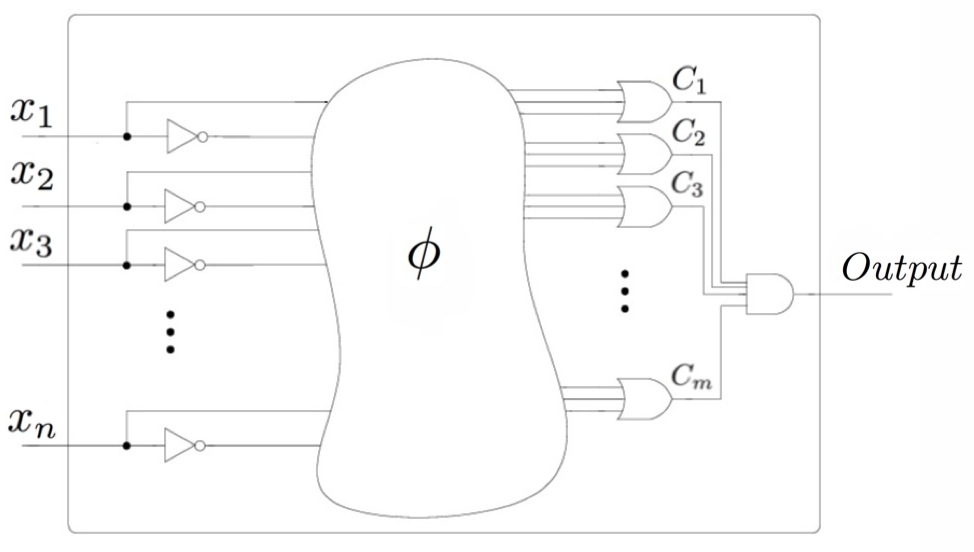
\includegraphics[width=0.9\textwidth]{figures/circuitLabeled.jpg}

\caption{A circuit describing {\sc Satisfiability}.}
\label{blackBoxSat}
\end{center}
\end{figure}
	
\FloatBarrier

%	<Paragraph> Provide complexity of {\sc Satisfiability}
The realization of {\sc Satisfiability} as a circuit reveals two aspects of this problem.  {\sc Satisfiability} can be implemented as a circuit with the number of gates proportional to the problem size.  The worst case verification for all $2^n$ possible witness candidates may be performed with the circuit in Figure \ref{blackBoxSat}.  This circuit consists of the hardware equivalent version of the {\sc Satisfiability} validator {\sc CheckSat}, as shown in Chapter 1.  
	
\section{Evaluating {\sc Sat} Solvers}

%	<Paragraph> Overview of evaluation
	
	In this section, we describe the standards for encoding the {\sc Satisfiability} problem that we adopt.  The standards come from from the {\sc Satisfiability} Competition \cite{dimacsFormat, satcompetition}.  
	
	Next, we introduce a problem instance classification scheme for {\sc Satisfiability}.  Classification of {\sc Satisfiability} problem instances include random, combinatorial, and industrial {\sc Sat} instances \cite{satcompetition}.  Our experiment in Chapter 6 generates random $k$-{\sc Sat} inputs.

	\subsection{Input and output}
	
%		<Paragraph> {\sc Satisfiability} standards [provide] common interface
	
%  Conforming to standards allows datasets and common interfaces to be shared.  
 The {\sc Sat} Competition ranks implementations of solvers for evaluating {\sc Satisfiability} \cite{satcompetition}.  {\sc Sat} solvers are evaluated on three categories of input: industrial, combinatorial, and random instances.  The input and output standards for {\sc Satisfiability} allow common benchmarks for {\sc Sat} solvers.  We conform to the standards of this competition \url{http://www.satcompetition.org/}.  
 

	
		\subsubsection{Input}
		
%			<Paragraph> DIMACS CNF [provides] standard benchmark instances
DIMACS CNF provides a standard input for {\sc Satisfiability} \cite{dimacsFormat}.  The format permits sharing of existing {\sc Satisfiability} benchmarks by encoding {\sc Satisfiability} in conjunctive normal form (CNF).  We provide an example of this encoding in Section \ref{inputSection}.
		
		\subsubsection{Output}
		
%			<Paragraph> Sat Competition output [provides] standard output

{\sc Sat} Competition output consists of the status of a DIMACS CNF input instance \cite{satcompetition}.  The status is provided for the instance as either \texttt{SATISFIABLE}, \texttt{UNSATISFIABLE}, or \texttt{UNKNOWN}.  If an instance can be determined as satisfiable, then a witness satisfying the instance gets included with the output status.  We provide an example along with custom output logging in Section \ref{outputSection}.
	
	\subsection{Metrics for classifying {\sc Satisfiability}}

%		<Paragraph> Describe metrics
{\sc Sat} phase transition and {\sc Sat} backbones are two metrics for classifying {\sc Satisfiability}.  We will use these metrics in the next section for defining a collection of random $k$-{\sc Sat} instances.
		
%		<Paragraph> {\sc Sat} phase transition


The ratio of $m$ clauses to $n$ variables $\alpha = m/n$ provides a characterization where phase transitions may occur in the space of all $k$-CNF formula \cite{Doherty08thehandbook,Gent94thesat}.  The {\sc Sat} phase transition is a region where both satisfiable and unsatisfiable instances are likely \cite{Gent94thesat}.  This region frequently separates trivially satisfiable and frequently over-constrained unsatisfiable {\sc Satisfiable} problem instances.  {\sc Satisfiability} instances with low $\alpha$ are frequently under-constrained and trivially satisfiable; those instances with high $\alpha$ are frequently over-constrained and trivially unsatisfiable \cite{Gent94thesat}.
		
%		<Paragraph> {\sc Sat} backbones
\begin{definition}
{\sc Sat} backbones\\
{\sc Sat} backbones are the variable assignments present in all of the satisfying assignments to a {\sc Satisfiability} problem instance \cite{Zhang2001}. 

\end{definition}

{\sc Sat} backbones contain a set of variables that occur in all satisfiable witnesses for an input instance.  If there are no such variables in the set of all witnesses for a problem instance, then the set is empty.

	\subsection{{\sc Satisfiability} instances}
		
%		<Paragraph> Various methods for [constructing] {\sc Satisfiability} instances
There are several methods for generating {\sc Satisfiability} instances.  We consider three classes \cite{satcompetition}: random assignment, combinatorial problems, and industrial applications.
	
\subsubsection{Random {\sc Sat}}
%		<Paragraph> {\sc Satisfiability} instance [generated] from random assignment
A random $k$-{\sc Sat} instance \cite{wilsonKsat}, for fixed $m$ and $n$, is one drawn uniformly from the set of all $k$-CNF formulas having $m$ clauses and $n$ variables.

%Random $k$-{\sc Sat} are generated with \texttt{ksat.c} \cite{wilsonKsat}.  A hash of the clause representation ensures that all clauses are independent \cite{wilsonKsat}.
%During generation of these formulas a hash is implemented to ensure that the random assignments ensure independent clauses and non-redundant variable assignments.  
		
%		<Paragraph> {\sc Satisfiability} instance [constructed] as hard assignment

\subsubsection{Hard combinatorial {\sc Sat}}

Combinatorial problem instances are well known difficult benchmark cases.  These instances include games and graph theoretic problems represented as {\sc Satisfiability}. 
		
%		<Paragraph> {\sc Satisfiability} instance [applied] from real world problems
\subsubsection{Industrial {\sc Sat}}

Industrial processes apply {\sc Satisfiability} to solve real world problems, including circuit layout, planning, logistics, circuit fault testing, and many other industrial \textsf{NP-complete} problems.  Industrial {\sc Sat} applications often apply heuristics and approximation techniques to relax the problem.  This allows approximate solutions to be computed efficiently with respect to time.

\chapter{Existing molecular algorithms for {\sc Satisfiability}}

%<Paragraph> Introduce two molecular algorithms for {\sc Satisfiability}

In this chapter, we discuss two molecular algorithms for {\sc Satisfiability}.  These algorithms construct sets of all witnesses for {\sc Satisfiability} instances.  Lipton's algorithm requires a combinatorial space of all witness candidates to be constructed and then filters out invalid ones.  Ogihara and Ray's algorithm constructs a set of witness candidates throughout execution.  Following the description, we explore the physical implementations of---and simulation frameworks for---these algorithms.

\begin{table}[htdp]
\caption{Components of Boolean literals and equivalent literal representations.}
\begin{center}
\begin{tabular}{| c | c | c | c | c |}
\hline
\textbf{Literal} & \textbf{Variable} $(v)$ & \textbf{Polarity} $(P)$ & \textbf{DIMACS} $(\pm v)$ & \textbf{Condensed} $(v_P)$ \\ \hline	
$x_1$ & $1$ & $\texttt{T}$ & $1$ & $1_{\texttt{T}}$ \\
$\neg x_1$ & $1$ & $\texttt{F}$ & $-1$ & $1_{\texttt{F}}$ \\
$x_n$ & $n$ & $\texttt{T}$ & $n$ & $n_{\texttt{T}}$ \\
$\neg x_n$ & $n$ & $\texttt{F}$ & $-n$ & $n_{\texttt{F}}$ \\ \hline
\end{tabular}
\end{center}
\label{equivalentLiteralTable}
\end{table}%

The algorithm definitions and example traces use the literal conventions listed in Table \ref{equivalentLiteralTable}.  Table \ref{equivalentLiteralTable} lists components of a literal (variable and polarity), along with equivalent forms (DIMACS and a condensed representation).  

In Chapter 1, witness candidates for {\sc Satisfiability} were represented as a bit-vector $B$.  Consider the equivalent representation for witness candidates in Figure \ref{equivalentWitnessRepresentations}.

\begin{figure}[htbp]
\begin{center}

	\begin{align*}
	B &= [0, 1, 0, 1 \rangle \\
	L &= \{ \neg x_1, x_2, \neg x_3, x_4 \} \\
	D &= \texttt{SFTFT}\\ 
	Z &= \texttt{S-1+2-3+4}\\ 
	\end{align*}

\caption{The bit-vector $B = [0, 1, 0, 1 \rangle$ can be represented as the set of literal assignments $L = \{ \neg x_1, x_2, \neg x_3, x_4 \}$.  A directed polarity string (D) with initial sequence (\texttt{S}), followed by a sequence of literals provides $D = \texttt{SFTFT}$.  A directed integer string (Z) consists of an initial sequence (\texttt{S}) followed by DIMACS literal assignments $Z =\texttt{S-1+2-3+4}$. }
\label{equivalentWitnessRepresentations}
\end{center}
\end{figure}

\FloatBarrier

We use the directed string notation (representation $D$ in Figure \ref{equivalentWitnessRepresentations}) as shorthand for a directed oligonucleotide.  The directed string representation $D$ can be indexed by the variable $v$ using the condensed literal from Table \ref{equivalentLiteralTable}.  In Lipton's algorithm, literal configurations for a variable $v$ get extracted directly ($v_{\texttt{T}}$ or $v_{\texttt{F}}$).

Ogihara and Ray's algorithm extracts satisfying literal configurations from an ordered clause $(a, b, c)$.  We use the condensed literal notation $v_P$ to indicate the assignment (either \texttt{T} or \texttt{F}) for the literal $v$.  We use the literal configuration $v_N$ to indicate any other non-satisfiable literal assignment to $v$.

In the discussion of the Distribution algorithm in Chapter 4, we use the directed integer notation (representation $Z$ in Figure \ref{equivalentWitnessRepresentations}) as shorthand for a directed sequence of integers.

Along with our shorthand representations ($D$ and $Z$) from Figure \ref{equivalentWitnessRepresentations}, we include a small combinatorial library corresponding to positive and negative literals.  Table \ref{smallCombinatorialLibrary} lists a mapping of literals to oligonucleotides used for literal matching and assignment.  


\begin{table}[htdp]
\caption{Positive and negative literal assignment and matching oligonucleotides.  }
\begin{center}
\begin{tabular}{|c|c|c|}
\hline
\textbf{Literal} & \textbf{Assignment} & \textbf{Matching} \\ \hline
$x_1$ & $5'-$\texttt{TTT}$-3'$ & $3'-$\texttt{AAA}$-5'$ \\ 
$\neg x_1$ & $5'-$\texttt{TTA}$-3'$ & $3'-$\texttt{AAT}$-5'$ \\ \hline
$x_2$ & $5'-$\texttt{CTT}$-3'$ & $3'-$\texttt{GAA}$-5'$ \\ 
$\neg x_2$ & $5'-$\texttt{ATT}$-3'$ & $3'-$\texttt{TAA}$-5'$ \\ \hline
$x_3$ & $5'-$\texttt{ATG}$-3'$ & $3'-$\texttt{TAC}$-5'$ \\ 
$\neg x_3$ & $5'-$\texttt{GTT}$-3'$ & $3'-$\texttt{CAA}$-5'$ \\ \hline
$x_4$ & $5'-$\texttt{TCT}$-3'$ & $3'-$\texttt{AGA}$-5'$ \\ 
$\neg x_4$ & $5'-$\texttt{CCT}$-3'$ & $3'-$\texttt{GGA}$-5'$ \\ \hline
$x_5$ & $5'-$\texttt{ACT}$-3'$ & $3'-$\texttt{TGA}$-5'$ \\ 
$\neg x_5$ & $5'-$\texttt{GCT}$-3'$ & $3'-$\texttt{CGA}$-5'$ \\ \hline
Start & $5'-$\texttt{TTG}$-3'$ & $3'-$\texttt{AAC}$-5'$ \\ \hline
\end{tabular}
\end{center}
\label{smallCombinatorialLibrary}
\end{table}%

\FloatBarrier

The examples throughout this report use this combinatorial library designed with codons.  Larger combinatorial libraries \cite{dnaComputingModels2008} take multiple considerations for the genetic encoding, including uniform melting temperature and non-self complementary sequences.  Codons provide redundant encodings that we exploit for a small library.   


\section{Lipton's algorithm for {\sc Satisfiability}}

%	<Paragraph> Introduce Lipton's algorithm

Introduced in 1995 by Richard Lipton \cite{Lipton95usingdna}, this algorithm filters satisfiable witnesses from a combinatorial space of all witness candidates.  Lipton's algorithm is analogous to a conventional brute-force search for all witnesses of a {\sc Satisfiability} instance.

Lipton's algorithm (Algorithm \ref{liptonAlgorithm}) first constructs a combinatorial space $T$ containing oligonucleotide configurations for all potential witness candidates.  The algorithm iterates over each of the clauses $C$ in $\phi$.  

From each clause $C$, each of the literals contained within each clause $C$ get filtered to satisfiable witnesses.  The contents of $T$ get filtered by incrementally extracting those literals that satisfy the current clause.  The next iteration filters witnesses that satisfy the previous clauses from $T$ and the literal contents from $C$.  The algorithm terminates with a set of witnesses $T$ for the CNF input $\phi$.  If $\phi$ is unsatisfiable, then $T = \emptyset$.  

% We iterate over each of the clauses in $\phi$.  Each clause iteration filters the contents of the tube $T$ to only witnesses that satisfy the current clause.  

	
\begin{figure}[htbp]
\begin{center}
	\begin{pseudocode}{Lipton's Algorithm}{\phi}
	T \GETS \text{{\sc Combinatorial Generate}}(n) \\
	\FOREACH \text{clause } C \text{ in } \phi \DO
		\BEGIN
		T_c \GETS \emptyset \\
		\FOREACH \text{literal } v \text{ in } C \DO
			\BEGIN
				\IF v \text{ is a positive literal} \THEN
					\BEGIN
						T_P \GETS \text{extract}(T, v_{\texttt{T}})\\
						T_c \GETS \text{mix}(T_P, T_c)						
					\END
				\ELSE
					\BEGIN
						T_N \GETS \text{extract}(T, v_{\texttt{F}})\\
						T_c \GETS \text{mix}(T_N, T_c)						
					\END
			\END
		\\
		T \GETS \text{purify(}T_c\text{)} \\
		\END
	\\
	\RETURN{\text{detect}(T)}
	\end{pseudocode}

\caption{{\sc Lipton's Algorithm} iterates over each of the $m$ clauses.  The contents of $T_C$ grows incrementally with configurations from $T$ that satisfy the literal $v$.  Once the entire clause $C$ has been evaluated, $T_C$ contains configurations that witness the observed conditions.  The contents of $T_C$ are stored as $T$ for the next clause; $T$ now contains configurations that witness all previous clauses.  Once complete, the tube $T$ contains all witnesses for $\phi$, if any witnesses exist.}
\label{liptonAlgorithm}
\end{center}
\end{figure}


\FloatBarrier

	\subsection{Description of Lipton's algorithm}
		
%		<Paragraph> Describe setup
The function {\sc Combinatorial Generate} (Algorithm \ref{combinatorialGenerate}) implements the split-mix synthesis technique \cite{furka1982, furkaBook}.  {\sc Combinatorial Generate} returns a tube $T_{comb}$ consisting of oligonucleotides that represent all $2^n$ distinct witness candidates.  The tube $T_{comb}$ begins with an initial medium denoted by \texttt{S}.  An iterative loop extends $T_{comb}$ using split-mix synthesis.  Each split corresponds with appending the tubes with a true (\texttt{T}) and false (\texttt{F}) assignment.  The two tubes are mixed and purified to contain equimolar portions of each witness candidate.  




\begin{figure}[htbp]
\begin{center}

	\begin{pseudocode}{Combinatorial Generate}{n}
		T_{comb} \GETS \emptyset \\
		T_{comb} \GETS \text{mix(}T_{comb}, \texttt{S} \text{)} \\ 
	
		\FOR v \GETS 1 \text{ to } n \DO
			\BEGIN
			
			[T_1,T_2] \GETS \text{split(} T_{comb}\text{)}\\
			T_1 \GETS \text{append(}T_1, v_{\texttt{T}} \text{)}\\
			T_2 \GETS \text{append(}T_2, v_{\texttt{F}} \text{)}\\
			T_{comb} \GETS \text{mix(}T_1,T_2\text{)}\\
		\END
		\\
		\RETURN {T_{comb}}
	\end{pseudocode}

\caption{{\sc Combinatorial Generate} constructs a combinatorial space consisting of $2^n$ molecular configurations in polynomial time.}
\label{combinatorialGenerate}
\end{center}
\end{figure}

\FloatBarrier

Let us consider an example execution of {\sc Combinatorial Generate} with $n = 2$.

\noindent The tube $T_{comb}$ begins as an empty tube.  A start configuration \texttt{S} initiates the tube $T_{comb}$ with a medium for combinatorial synthesis.

\noindent We begin with the initial contents

\begin{center}
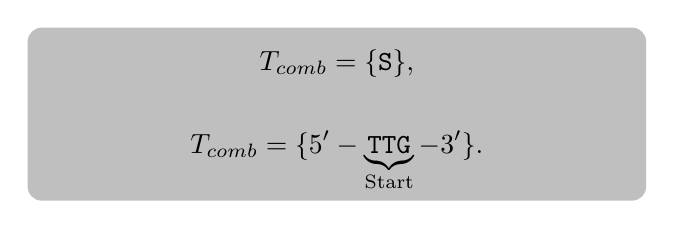
\begin{tikzpicture}
\node[fill=lightgray, rounded corners=5pt, text width=3in]{
\[
T_{comb} = \{ \texttt{S} \},
\]

\[
T_{comb} = \{ 5'-\underbrace{\texttt{TTG}}_{\text{Start}}-3' \}.
\]
};
\end{tikzpicture}
\end{center}

\noindent Iteration $v = 1$:

First, split the contents of $T_{comb}$.  We have

\begin{center}
\begin{tikzpicture}
\node[fill=gray, rounded corners=5pt, text width=6in]{

	\makebox[\textwidth][r]{
		\begin{minipage}[t]{0.5\textwidth}
			\begin{center}
			\begin{tikzpicture}
			\node[fill=lightgray, rounded corners=5pt, text width=2.5in]{
				\[
					T_1 = \{ \texttt{S} \}
				\]
				\[
					T_1 = \{ 5'-\underbrace{\texttt{TTG}}_{\text{Start}}-3' \}
				\]
			};
			\end{tikzpicture}
			\end{center}
		\end{minipage}				
		\begin{minipage}[t]{0.5\textwidth}
			\begin{center}
			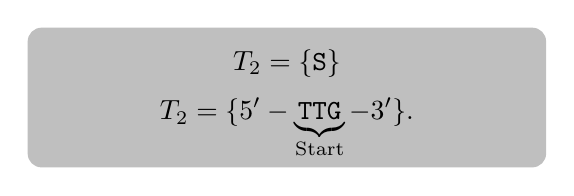
\begin{tikzpicture}
			\node[fill=lightgray, rounded corners=5pt, text width=2.5in]{
				\[
					T_2 = \{ \texttt{S} \}
				\]
				\[
					T_2 = \{ 5'-\underbrace{\texttt{TTG}}_{\text{Start}}-3' \}.
				\]
			};
			\end{tikzpicture}
			\end{center}
		\end{minipage}		
	}
};
\end{tikzpicture}
\end{center}
\hspace{1em}

Next, append each of the tubes with a positive (\texttt{T}) and negative (\texttt{F}) assignment for the literal $v_1$.  We have

\begin{center}
\begin{tikzpicture}
\node[fill=gray, rounded corners=5pt, text width=6in]{
	\makebox[\textwidth][r]{
		\begin{minipage}[t]{0.5\textwidth}
			\begin{center}
			\begin{tikzpicture}
			\node[fill=lightgray, rounded corners=5pt, text width=2.5in]{
				\[
					T_1 = \{ \texttt{ST} \}
				\]
				\[
					T_1 = \{ 5'-\underbrace{\texttt{TTG}}_{\text{Start}}\cdot\underbrace{\texttt{TTT}}_{ x_{1}}-3' \}
				\]
			};
			\end{tikzpicture}
			\end{center}			
		\end{minipage}				
		\begin{minipage}[t]{0.5\textwidth}
			\begin{center}
			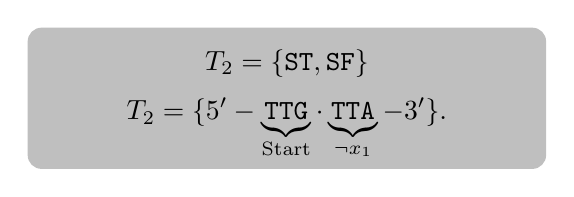
\begin{tikzpicture}
			\node[fill=lightgray, rounded corners=5pt, text width=2.5in]{			
				\[
					T_2 = \{\texttt{ST}, \texttt{SF}\}
				\]
				\[
					T_2 = \{ 5'-\underbrace{\texttt{TTG}}_{\text{Start}}\cdot\underbrace{\texttt{TTA}}_{\neg x_{1}}-3' \}.		
				\]
			};
			\end{tikzpicture}
			\end{center}		
		\end{minipage}		
	}
};
\end{tikzpicture}
\end{center}

\hspace{1em}

Mix the contents of $T_1$ and $T_2$ to form $T_{comb}$ for the next iteration.  We have

\begin{center}
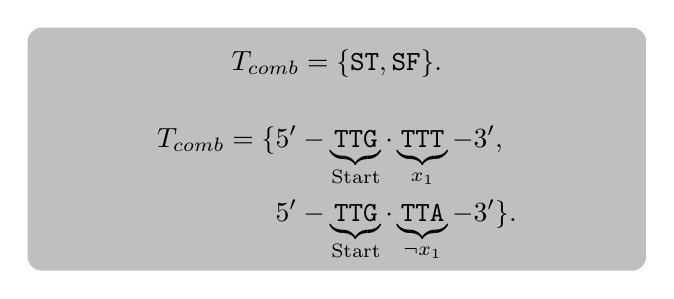
\begin{tikzpicture}
\node[fill=lightgray, rounded corners=5pt, text width=3in]{
\[
T_{comb} = \{\texttt{ST}, \texttt{SF}\}.
\]
\begin{align*}
T_{comb} = \{&5'-\underbrace{\texttt{TTG}}_{\text{Start}}\cdot\underbrace{\texttt{TTT}}_{ x_{1}}-3',\\
&5'-\underbrace{\texttt{TTG}}_{\text{Start}}\cdot\underbrace{\texttt{TTA}}_{\neg x_{1}}-3' \}.
\end{align*}
};
\end{tikzpicture}
\end{center}

\noindent Iteration $v = 2$:

Split the contents of $T_{comb}$.  We have

\begin{center}
\begin{tikzpicture}
\node[fill=gray, rounded corners=5pt, text width=6in]{
	\makebox[\textwidth][l]{
		\begin{minipage}[t]{0.5\textwidth}
			\begin{center}
			\begin{tikzpicture}
			\node[fill=lightgray, rounded corners=5pt, text width=2.5in]{		
				\[
				T_1 = \{\texttt{ST}, \texttt{SF}\}
				\]
				\begin{align*}
				T_{1} = \{&5'-\underbrace{\texttt{TTG}}_{\text{Start}}\cdot\underbrace{\texttt{TTT}}_{ x_{1}}-3',\\
						  &5'-\underbrace{\texttt{TTG}}_{\text{Start}}\cdot\underbrace{\texttt{TTA}}_{\neg x_{1}}-3' \}
				\end{align*}
			};
			\end{tikzpicture}
			\end{center}				
		\end{minipage}				
		\begin{minipage}[t]{0.5\textwidth}
			\begin{center}
			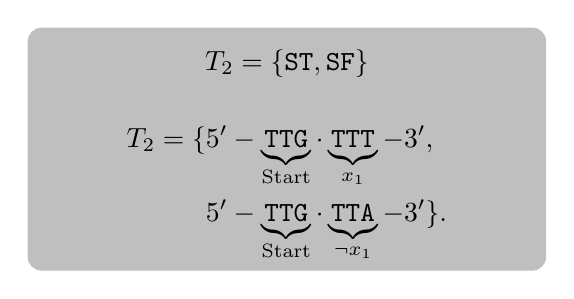
\begin{tikzpicture}
			\node[fill=lightgray, rounded corners=5pt, text width=2.5in]{
				\[
				 T_2 = \{\texttt{ST}, \texttt{SF}\}
				\]
				\begin{align*}	
				T_{2} = \{&5'-\underbrace{\texttt{TTG}}_{\text{Start}}\cdot\underbrace{\texttt{TTT}}_{ x_{1}}-3',\\
						  &5'-\underbrace{\texttt{TTG}}_{\text{Start}}\cdot\underbrace{\texttt{TTA}}_{\neg x_{1}}-3' \}.
				\end{align*}
			};
			\end{tikzpicture}
			\end{center}				
		\end{minipage}		
	}
};
\end{tikzpicture}
\end{center}
	
\hspace{1em}

Next, append each of the tubes with a positive (\texttt{T}) and negative (\texttt{F}) assignment for the literal $v_2$.  We have

\begin{center}
\begin{tikzpicture}
\node[fill=gray, rounded corners=5pt, text width=6in]{
	\makebox[\textwidth][r]{
		\begin{minipage}[t]{0.5\textwidth}
			\begin{center}
			\begin{tikzpicture}
			\node[fill=lightgray, rounded corners=5pt, text width=2.5in]{		
				\[
				T_1 = \{\texttt{STT}, \texttt{SFT}\}
				\]
				\begin{align*}
				T_{1} = \{&5'-\underbrace{\texttt{TTG}}_{\text{Start}}\cdot\underbrace{\texttt{TTT}}_{ x_{1}}\cdot\underbrace{\texttt{CTT}}_{ x_{2}}-3',\\
						  &5'-\underbrace{\texttt{TTG}}_{\text{Start}}\cdot\underbrace{\texttt{TTA}}_{\neg x_{1}}\cdot\underbrace{\texttt{CTT}}_{ x_{2}}-3' \}
				\end{align*}
			};
			\end{tikzpicture}
			\end{center}				
		\end{minipage}				
		\begin{minipage}[t]{0.5\textwidth}
			\begin{center}
			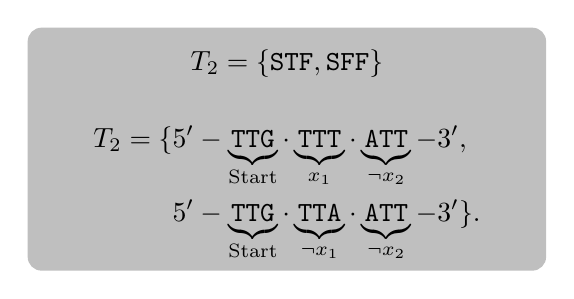
\begin{tikzpicture}
			\node[fill=lightgray, rounded corners=5pt, text width=2.5in]{
				\[
				T_2 = \{\texttt{STF}, \texttt{SFF}\}		
				\]
				\begin{align*}	
				T_{2} = \{&5'-\underbrace{\texttt{TTG}}_{\text{Start}}\cdot\underbrace{\texttt{TTT}}_{ x_{1}}\cdot\underbrace{\texttt{ATT}}_{\neg x_{2}}-3',\\
						  &5'-\underbrace{\texttt{TTG}}_{\text{Start}}\cdot\underbrace{\texttt{TTA}}_{\neg x_{1}}\cdot\underbrace{\texttt{ATT}}_{\neg x_{2}}-3' \}.
				\end{align*}
			};
			\end{tikzpicture}
			\end{center}				
		\end{minipage}		
	}
};
\end{tikzpicture}
\end{center}
\hspace{1em}

Mix the contents of $T_1$ and $T_2$ to form $T_{comb}$ for the final iteration.  The algorithm {\sc Combinatorial Generate} returns the following tube

\begin{center}
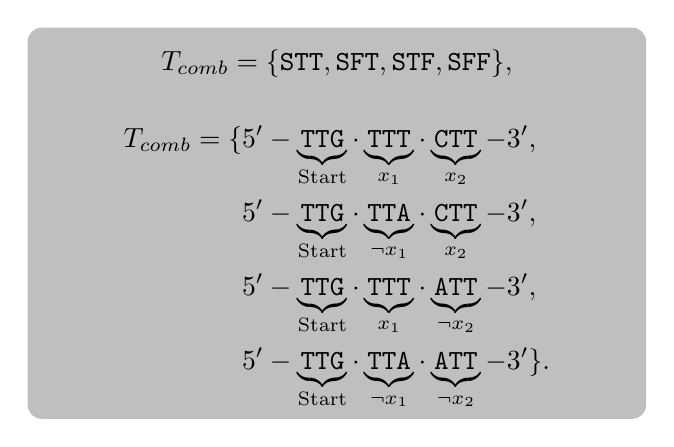
\begin{tikzpicture}
\node[fill=lightgray, rounded corners=5pt, text width=3in]{
	\[
	T_{comb} = \{\texttt{STT}, \texttt{SFT}, \texttt{STF}, \texttt{SFF}\},
	\]
	\begin{align*}
	T_{comb} = \{&5'-\underbrace{\texttt{TTG}}_{\text{Start}}\cdot\underbrace{\texttt{TTT}}_{ x_{1}}\cdot\underbrace{\texttt{CTT}}_{ x_{2}}-3',\\
			  &5'-\underbrace{\texttt{TTG}}_{\text{Start}}\cdot\underbrace{\texttt{TTA}}_{\neg x_{1}}\cdot\underbrace{\texttt{CTT}}_{ x_{2}}-3',\\
			  &5'-\underbrace{\texttt{TTG}}_{\text{Start}}\cdot\underbrace{\texttt{TTT}}_{ x_{1}}\cdot\underbrace{\texttt{ATT}}_{\neg x_{2}}-3',\\
			  &5'-\underbrace{\texttt{TTG}}_{\text{Start}}\cdot\underbrace{\texttt{TTA}}_{\neg x_{1}}\cdot\underbrace{\texttt{ATT}}_{\neg x_{2}}-3' \}.
	\end{align*}
};
\end{tikzpicture}
\end{center}	
%%%%%%%%%%%%%%%%%

{\sc Combinatorial Generate} generates all witness candidates for a {\sc Satisfiability} instance.  Lipton's algorithm filters, from a combinatorial space $T$, configurations that represent witnesses for the input $\phi$.

	\subsection{Detailed trace of Lipton's algorithm}	
%	<Paragraph> Introduce pseudocode
Appendix B lists a detailed execution trace for Lipton's algorithm.

%%%%%%%%%%%%%%%%%%%%%%%%%%%%%%%%%

\section{Ogihara and Ray's algorithm for {\sc Satisfiability}}

%	<Paragraph> Introduce Ogihara and Ray's algorithm

Ogihara and Ray's algorithm (Algorithm \ref{ogiharaRayAlgorithm}) consist of a breadth-first evaluation of clauses from a CNF formula \cite{Ogihara:1996:BFS:898228,Ogihara97dna-basedparallel}.  The algorithm constructs a set of witness candidates based on a parse of a 3-CNF formula.  In this section, we describe the preconditions and execution of Ogihara and Ray's algorithm.

%		<Paragraph> Describe execution

\begin{figure}[htbp]
	\renewcommand{\figurename}{Algorithm}
	\renewcommand{\thepseudocode}{\ref{ogiharaRayAlgorithm}}
	
	\begin{center}

	\begin{pseudocode}[shadowbox]{Ogihara and Ray's Algorithm}{\phi}
	
	\text{// Input $\phi$ consists of $n$ variables.}\\
	\text{// Each clause $C$ contains ordered literals $(a,b,c)$.}\\
	\text{// Extract literals using the condensed notation $v_P$, where: }\\
	\text{// \hspace{1em} $v_P$ matches the literal, and $v_N$ matches the negated literal.}\\
	\\
	T \GETS \{ \texttt{STT}, \texttt{STF}, \texttt{SFT},  \texttt{SFF}\} \\
	
	\FOR v \GETS 3 \text{ to } n \DO
		\BEGIN
		[T_P, T_N] \GETS \text{split}(T)\\
	
		\FOREACH \text{clause } C \text{ in } \phi \DO
			\BEGIN
				(a, b, c) \GETS C\\
				\IF v_{\texttt{T}} = c  \THEN
					\BEGIN
						T_{P1} \GETS \text{extract}(T_N, a_P)\\
						T_{N1} \GETS \text{extract}(T_N, a_N)\\				
						T_{P2} \GETS \text{extract}(T_{N1}, b_P)\\
						T_{N} \GETS \text{mix}(T_{P1}, T_{P2})\\
						T_{N} \GETS \text{purify(}T_{N}\text{)}					
					\END \\  
				\IF v_{\texttt{F}} = c \THEN
					\BEGIN
						T_{P1} \GETS \text{extract}(T_P, a_P)\\
						T_{N1} \GETS \text{extract}(T_P, a_N)\\				
						T_{P2} \GETS \text{extract}(T_{N1}, b_P)\\
						T_{P} \GETS \text{mix}(T_{P1}, T_{P2})\\
						T_{P} \GETS \text{purify(}T_{P}\text{)} 						
					\END\\
			\END\\
			T_P \GETS \text{append}(T_P, v_{\texttt{T}})\\
			T_N \GETS \text{append}(T_N, v_{\texttt{F}})\\
			T \GETS \text{mix}(T_P, T_N)\\
			T \GETS \text{purify(}T\text{)} \\									
		\END\\
	\RETURN{\text{detect}(T)}
	\end{pseudocode}

\caption{{\sc Ogihara and Ray's Algorithm} evaluates each subsequent variable and determines possible assignments.  The possible assignments for the variables $a$ and $b$ get extracted if $c$ matches the current variable $v$.  Effectively pruning only potential solutions.  These potential solutions $T_P$ and $T_N$ get appended with the positive or negative string assignments.  The algorithm continues until each variable gets evaluated.  The remaining space $T$ contains all solutions for the CNF instance $\phi$ after the algorithm terminates.}
\label{ogiharaRayAlgorithm}
\end{center}
\end{figure}

\FloatBarrier

\subsection{Description of Ogihara and Ray's algorithm}
		
Ogihara and Ray's algorithm begins with four initial witness candidates, we have

\begin{center}
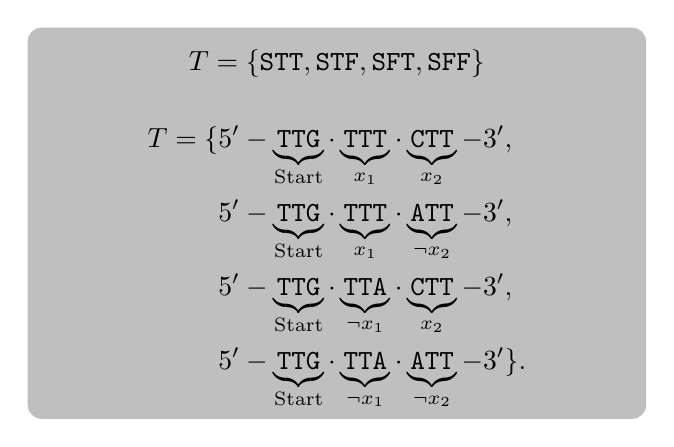
\begin{tikzpicture}
\node[fill=lightgray, rounded corners=5pt, text width=3in]{
	\[
	T = \{ \texttt{STT}, \texttt{STF}, \texttt{SFT}, \texttt{SFF}\}
	\]
	\begin{align*}
	T = \{ &5'-\underbrace{\texttt{TTG}}_{\text{Start}}\cdot\underbrace{\texttt{TTT}}_{ x_{1}}\cdot\underbrace{\texttt{CTT}}_{ x_{2}}-3',\\
		   &5'-\underbrace{\texttt{TTG}}_{\text{Start}}\cdot\underbrace{\texttt{TTT}}_{ x_{1}}\cdot\underbrace{\texttt{ATT}}_{\neg x_{2}}-3',\\
		   &5'-\underbrace{\texttt{TTG}}_{\text{Start}}\cdot\underbrace{\texttt{TTA}}_{\neg x_{1}}\cdot\underbrace{\texttt{CTT}}_{ x_{2}}-3',\\
		   &5'-\underbrace{\texttt{TTG}}_{\text{Start}}\cdot\underbrace{\texttt{TTA}}_{\neg x_{1}}\cdot\underbrace{\texttt{ATT}}_{\neg x_{2}}-3'\}.
	\end{align*}
};
\end{tikzpicture}
\end{center}

For each clause $C = (x_i \vee x_j \vee x_k)$, we have that $1 \leq i < j < k \leq n$.  As an example, let us evaluate the clause
\[
C = x_1 \vee \neg x_2 \vee \neg x_3.
\]

\noindent On the first iteration, we compare the third ordered literal $c$ with $x_3$.  Since $c = \neg x_3$, extract configurations that satisfy $a \vee b$.  

\begin{center}
\begin{tikzpicture}
\node[fill=gray, rounded corners=5pt, text width=6in]{
	\makebox[\textwidth][r]{
		\begin{minipage}[t]{0.5\textwidth}
			\begin{center}
			\begin{tikzpicture}
			\node[fill=lightgray, rounded corners=5pt, text width=2.5in]{		
				\[
				T_P = \{ \texttt{STT}, \texttt{STF}, \texttt{SFT}, \texttt{SFF}\}
				\]
				\begin{align*}
				T_P = \{ &5'-\underbrace{\texttt{TTG}}_{\text{Start}}\cdot\underbrace{\texttt{TTT}}_{ x_{1}}\cdot\underbrace{\texttt{CTT}}_{ x_{2}}-3',\\
					   &5'-\underbrace{\texttt{TTG}}_{\text{Start}}\cdot\underbrace{\texttt{TTT}}_{ x_{1}}\cdot\underbrace{\texttt{ATT}}_{\neg x_{2}}-3',\\
					   &5'-\underbrace{\texttt{TTG}}_{\text{Start}}\cdot\underbrace{\texttt{TTA}}_{\neg x_{1}}\cdot\underbrace{\texttt{CTT}}_{ x_{2}}-3',\\
					   &5'-\underbrace{\texttt{TTG}}_{\text{Start}}\cdot\underbrace{\texttt{TTA}}_{\neg x_{1}}\cdot\underbrace{\texttt{ATT}}_{\neg x_{2}}-3'\},
				\end{align*}
			};
			\end{tikzpicture}
			\end{center}				
		\end{minipage}				
		\begin{minipage}[t]{0.5\textwidth}
			\begin{center}
			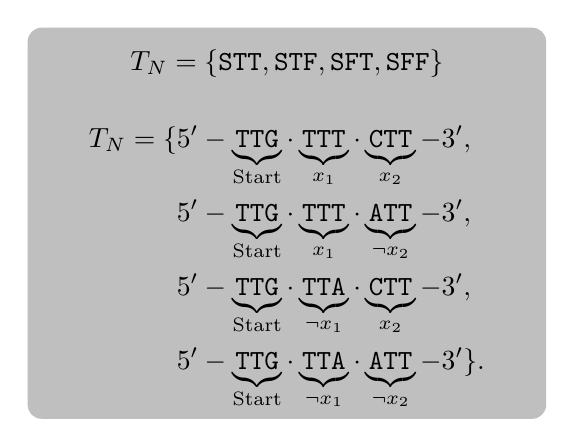
\begin{tikzpicture}
			\node[fill=lightgray, rounded corners=5pt, text width=2.5in]{
				\[
				T_N = \{ \texttt{STT}, \texttt{STF}, \texttt{SFT}, \texttt{SFF}\}		
				\]
				\begin{align*}	
				T_N = \{ &5'-\underbrace{\texttt{TTG}}_{\text{Start}}\cdot\underbrace{\texttt{TTT}}_{ x_{1}}\cdot\underbrace{\texttt{CTT}}_{ x_{2}}-3',\\
					   &5'-\underbrace{\texttt{TTG}}_{\text{Start}}\cdot\underbrace{\texttt{TTT}}_{ x_{1}}\cdot\underbrace{\texttt{ATT}}_{\neg x_{2}}-3',\\
					   &5'-\underbrace{\texttt{TTG}}_{\text{Start}}\cdot\underbrace{\texttt{TTA}}_{\neg x_{1}}\cdot\underbrace{\texttt{CTT}}_{ x_{2}}-3',\\
					   &5'-\underbrace{\texttt{TTG}}_{\text{Start}}\cdot\underbrace{\texttt{TTA}}_{\neg x_{1}}\cdot\underbrace{\texttt{ATT}}_{\neg x_{2}}-3'\}.
				\end{align*}
			};
			\end{tikzpicture}
			\end{center}				
		\end{minipage}		
	}
};
\end{tikzpicture}
\end{center}
	
\hspace{1em}

\noindent From $T$, select configurations that satisfy $a_P = a_{\texttt{T}}$

\begin{center}
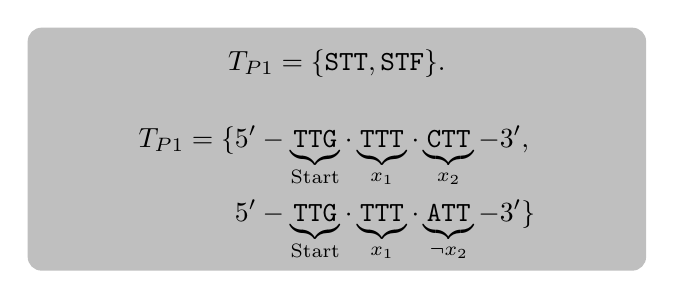
\begin{tikzpicture}
\node[fill=lightgray, rounded corners=5pt, text width=3in]{
	\[
	T_{P1} = \{ \texttt{STT}, \texttt{STF} \}.
	\]
	\begin{align*}
	T_{P1} = \{ &5'-\underbrace{\texttt{TTG}}_{\text{Start}}\cdot\underbrace{\texttt{TTT}}_{ x_{1}}\cdot\underbrace{\texttt{CTT}}_{ x_{2}}-3', \\
				&5'-\underbrace{\texttt{TTG}}_{\text{Start}}\cdot\underbrace{\texttt{TTT}}_{ x_{1}}\cdot\underbrace{\texttt{ATT}}_{\neg x_{2}}-3'\}
	\end{align*}
};
\end{tikzpicture}
\end{center}

\noindent From $T$, Select configurations that satisfy $a_N = a_{\texttt{F}}$

\begin{center}
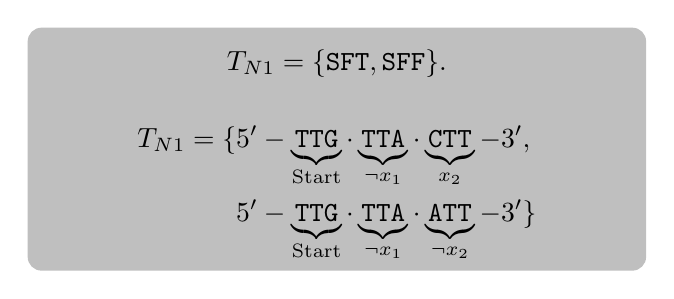
\begin{tikzpicture}
\node[fill=lightgray, rounded corners=5pt, text width=3in]{
	\[
	T_{N1} = \{ \texttt{SFT}, \texttt{SFF} \}.
	\]
	\begin{align*}
	T_{N1} = \{ &5'-\underbrace{\texttt{TTG}}_{\text{Start}}\cdot\underbrace{\texttt{TTA}}_{\neg x_{1}}\cdot\underbrace{\texttt{CTT}}_{ x_{2}}-3',\\
				&5'-\underbrace{\texttt{TTG}}_{\text{Start}}\cdot\underbrace{\texttt{TTA}}_{\neg x_{1}}\cdot\underbrace{\texttt{ATT}}_{\neg x_{2}}-3'\}
	\end{align*}
};
\end{tikzpicture}
\end{center}

\noindent From $T_{N1}$, select configurations that satisfy $b_P = b_{\texttt{F}}$
\begin{center}
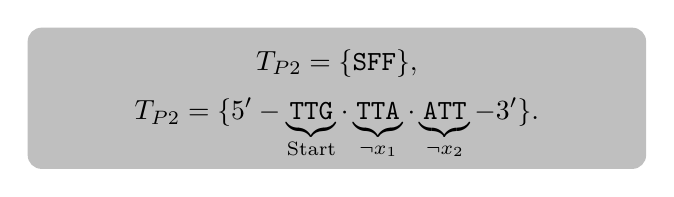
\begin{tikzpicture}
\node[fill=lightgray, rounded corners=5pt, text width=3in]{
	\[
	T_{P2} = \{ \texttt{SFF} \},
	\]
	\[
	T_{P2} = \{ 5'-\underbrace{\texttt{TTG}}_{\text{Start}}\cdot\underbrace{\texttt{TTA}}_{\neg x_{1}}\cdot\underbrace{\texttt{ATT}}_{\neg x_{2}}-3'\}.
	\]
};
\end{tikzpicture}
\end{center}

\noindent Mix the contents of $T_{P1}$ and $T_{P2}$ as the contents of $T_P$

\begin{center}
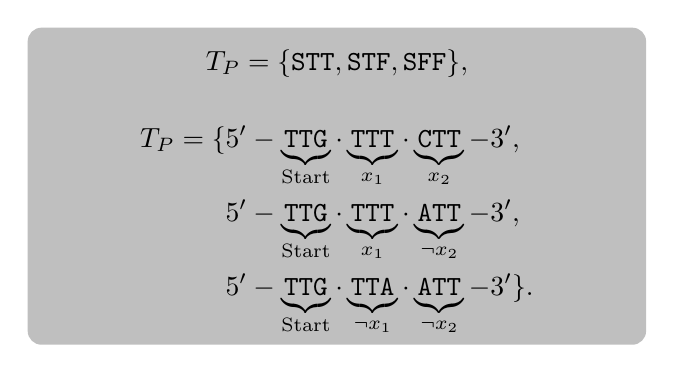
\begin{tikzpicture}
\node[fill=lightgray, rounded corners=5pt, text width=3in]{
	\[
	T_P = \{ \texttt{STT}, \texttt{STF}, \texttt{SFF} \},
	\]
	\begin{align*}
	T_P = \{ &5'-\underbrace{\texttt{TTG}}_{\text{Start}}\cdot\underbrace{\texttt{TTT}}_{ x_{1}}\cdot\underbrace{\texttt{CTT}}_{ x_{2}}-3', \\
			 &5'-\underbrace{\texttt{TTG}}_{\text{Start}}\cdot\underbrace{\texttt{TTT}}_{ x_{1}}\cdot\underbrace{\texttt{ATT}}_{\neg x_{2}}-3', \\
			 &5'-\underbrace{\texttt{TTG}}_{\text{Start}}\cdot\underbrace{\texttt{TTA}}_{\neg x_{1}}\cdot\underbrace{\texttt{ATT}}_{\neg x_{2}}-3'\}.
	\end{align*}
};
\end{tikzpicture}
\end{center}

\noindent We have the tubes

\begin{center}
\begin{tikzpicture}
\node[fill=gray, rounded corners=5pt, text width=6in]{
	\makebox[\textwidth][r]{
		\begin{minipage}[t]{0.5\textwidth}
			\begin{center}
			\begin{tikzpicture}
			\node[fill=lightgray, rounded corners=5pt, text width=2.5in]{		
				\[
				T_P = \{ \texttt{STT}, \texttt{STF}, \texttt{SFF} \}
				\]
				\begin{align*}
				T_P = \{ &5'-\underbrace{\texttt{TTG}}_{\text{Start}}\cdot\underbrace{\texttt{TTT}}_{ x_{1}}\cdot\underbrace{\texttt{CTT}}_{ x_{2}}-3', \\
						 &5'-\underbrace{\texttt{TTG}}_{\text{Start}}\cdot\underbrace{\texttt{TTT}}_{ x_{1}}\cdot\underbrace{\texttt{ATT}}_{\neg x_{2}}-3', \\
						 &5'-\underbrace{\texttt{TTG}}_{\text{Start}}\cdot\underbrace{\texttt{TTA}}_{\neg x_{1}}\cdot\underbrace{\texttt{ATT}}_{\neg x_{2}}-3'\},\\
				\end{align*}
			};
			\end{tikzpicture}
			\end{center}				
		\end{minipage}		
		\begin{minipage}[t]{0.5\textwidth}
			\begin{center}
			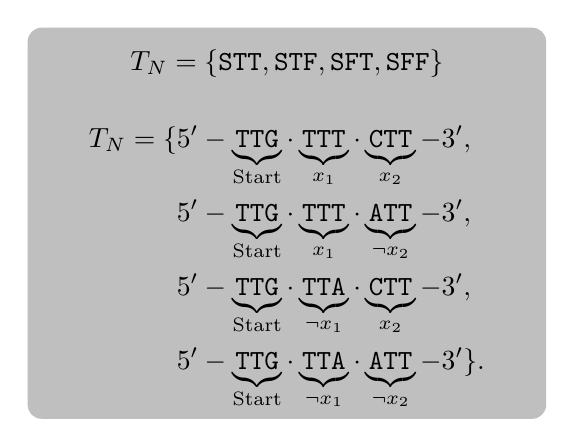
\begin{tikzpicture}
			\node[fill=lightgray, rounded corners=5pt, text width=2.5in]{		
				\[
				T_N = \{ \texttt{STT}, \texttt{STF}, \texttt{SFT}, \texttt{SFF}\}
				\]
				\begin{align*}
				T_N = \{ &5'-\underbrace{\texttt{TTG}}_{\text{Start}}\cdot\underbrace{\texttt{TTT}}_{ x_{1}}\cdot\underbrace{\texttt{CTT}}_{ x_{2}}-3',\\
					   &5'-\underbrace{\texttt{TTG}}_{\text{Start}}\cdot\underbrace{\texttt{TTT}}_{ x_{1}}\cdot\underbrace{\texttt{ATT}}_{\neg x_{2}}-3',\\
					   &5'-\underbrace{\texttt{TTG}}_{\text{Start}}\cdot\underbrace{\texttt{TTA}}_{\neg x_{1}}\cdot\underbrace{\texttt{CTT}}_{ x_{2}}-3',\\
					   &5'-\underbrace{\texttt{TTG}}_{\text{Start}}\cdot\underbrace{\texttt{TTA}}_{\neg x_{1}}\cdot\underbrace{\texttt{ATT}}_{\neg x_{2}}-3'\}.
				\end{align*}
			};
			\end{tikzpicture}
			\end{center}				
		\end{minipage}		
	}
};
\end{tikzpicture}
\end{center}

\hspace{1em}

\noindent Finally append assignments that satisfy the current literal with $T_P$ and $T_F$.

\begin{center}
\begin{tikzpicture}
\node[fill=gray, rounded corners=5pt, text width=6in]{
	\makebox[\textwidth][r]{
		\begin{minipage}[t]{0.5\textwidth}
			\begin{center}
			\begin{tikzpicture}
			\node[fill=lightgray, rounded corners=5pt, text width=2.5in]{		
				\begin{align*}
				T_P &= \text{append}(T_P, c_{\texttt{F}}) \\
					&= \{ \texttt{STTF}, \texttt{STFF}, \texttt{SFFF} \}
				\end{align*}
				\begin{align*}
				T_P = \{ &5'-\underbrace{\texttt{TTG}}_{\text{Start}}\cdot\underbrace{\texttt{TTT}}_{ x_{1}}\cdot\underbrace{\texttt{CTT}}_{ x_{2}}\cdot\underbrace{\texttt{GTT}}_{\neg x_{3}}-3',\\
						 &5'-\underbrace{\texttt{TTG}}_{\text{Start}}\cdot\underbrace{\texttt{TTT}}_{ x_{1}}\cdot\underbrace{\texttt{ATT}}_{\neg x_{2}}\cdot\underbrace{\texttt{GTT}}_{\neg x_{3}}-3',\\
						 &5'-\underbrace{\texttt{TTG}}_{\text{Start}}\cdot\underbrace{\texttt{TTA}}_{\neg x_{1}}\cdot\underbrace{\texttt{ATT}}_{\neg x_{2}}\cdot\underbrace{\texttt{GTT}}_{\neg x_{3}}-3' \}
				\end{align*}
			};
			\end{tikzpicture}
			\end{center}
		\end{minipage}
		
		\begin{minipage}[t]{0.5\textwidth}
			\begin{center}
			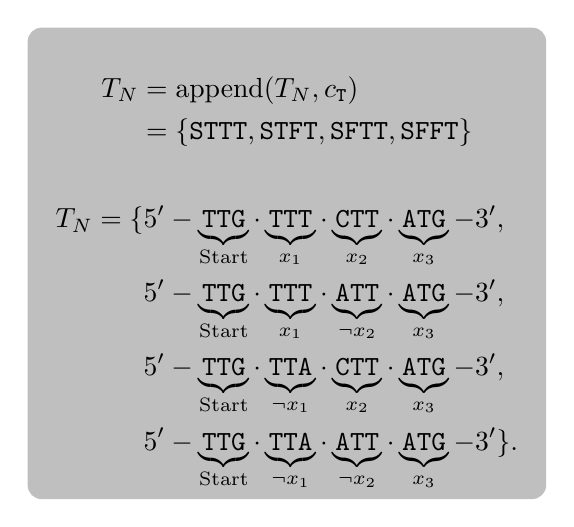
\begin{tikzpicture}
			\node[fill=lightgray, rounded corners=5pt, text width=2.5in]{
				\begin{align*}
				T_N &= \text{append}(T_N, c_{\texttt{T}}) \\
					&= \{ \texttt{STTT}, \texttt{STFT}, \texttt{SFTT}, \texttt{SFFT}\}
				\end{align*}
				\begin{align*}
				T_N = \{ &5'-\underbrace{\texttt{TTG}}_{\text{Start}}\cdot\underbrace{\texttt{TTT}}_{ x_{1}}\cdot\underbrace{\texttt{CTT}}_{ x_{2}}\cdot\underbrace{\texttt{ATG}}_{ x_{3}}-3',\\
						 &5'-\underbrace{\texttt{TTG}}_{\text{Start}}\cdot\underbrace{\texttt{TTT}}_{ x_{1}}\cdot\underbrace{\texttt{ATT}}_{\neg x_{2}}\cdot\underbrace{\texttt{ATG}}_{ x_{3}}-3',\\
						 &5'-\underbrace{\texttt{TTG}}_{\text{Start}}\cdot\underbrace{\texttt{TTA}}_{\neg x_{1}}\cdot\underbrace{\texttt{CTT}}_{ x_{2}}\cdot\underbrace{\texttt{ATG}}_{ x_{3}}-3',\\
						 &5'-\underbrace{\texttt{TTG}}_{\text{Start}}\cdot\underbrace{\texttt{TTA}}_{\neg x_{1}}\cdot\underbrace{\texttt{ATT}}_{\neg x_{2}}\cdot\underbrace{\texttt{ATG}}_{ x_{3}}-3'\}.
				\end{align*}
			};
			\end{tikzpicture}
			\end{center}
		\end{minipage}
	}
};
\end{tikzpicture}
\end{center}

\hspace{1em}

\noindent Mix the contents of $T_P$ and $T_N$ to form the set of configurations that witness the clause. 

\begin{center}
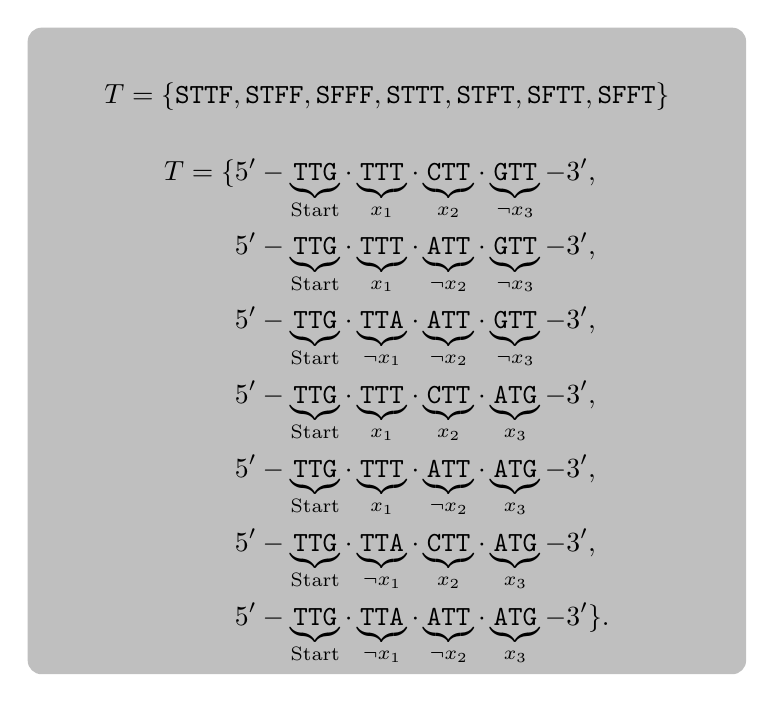
\begin{tikzpicture}
\node[fill=lightgray, rounded corners=5pt, text width=3.5in]{
	
	\[
	T = \{ \texttt{STTF}, \texttt{STFF}, \texttt{SFFF},  \texttt{STTT}, \texttt{STFT}, \texttt{SFTT}, \texttt{SFFT}\}
	\]
	\begin{align*}
	T = \{ &5'-\underbrace{\texttt{TTG}}_{\text{Start}}\cdot\underbrace{\texttt{TTT}}_{ x_{1}}\cdot\underbrace{\texttt{CTT}}_{ x_{2}}\cdot\underbrace{\texttt{GTT}}_{\neg x_{3}}-3',\\
		   &5'-\underbrace{\texttt{TTG}}_{\text{Start}}\cdot\underbrace{\texttt{TTT}}_{ x_{1}}\cdot\underbrace{\texttt{ATT}}_{\neg x_{2}}\cdot\underbrace{\texttt{GTT}}_{\neg x_{3}}-3',\\
		   &5'-\underbrace{\texttt{TTG}}_{\text{Start}}\cdot\underbrace{\texttt{TTA}}_{\neg x_{1}}\cdot\underbrace{\texttt{ATT}}_{\neg x_{2}}\cdot\underbrace{\texttt{GTT}}_{\neg x_{3}}-3',\\
		   &5'-\underbrace{\texttt{TTG}}_{\text{Start}}\cdot\underbrace{\texttt{TTT}}_{ x_{1}}\cdot\underbrace{\texttt{CTT}}_{ x_{2}}\cdot\underbrace{\texttt{ATG}}_{ x_{3}}-3',\\
		   &5'-\underbrace{\texttt{TTG}}_{\text{Start}}\cdot\underbrace{\texttt{TTT}}_{ x_{1}}\cdot\underbrace{\texttt{ATT}}_{\neg x_{2}}\cdot\underbrace{\texttt{ATG}}_{ x_{3}}-3',\\
		   &5'-\underbrace{\texttt{TTG}}_{\text{Start}}\cdot\underbrace{\texttt{TTA}}_{\neg x_{1}}\cdot\underbrace{\texttt{CTT}}_{ x_{2}}\cdot\underbrace{\texttt{ATG}}_{ x_{3}}-3',\\
		   &5'-\underbrace{\texttt{TTG}}_{\text{Start}}\cdot\underbrace{\texttt{TTA}}_{\neg x_{1}}\cdot\underbrace{\texttt{ATT}}_{\neg x_{2}}\cdot\underbrace{\texttt{ATG}}_{ x_{3}}-3'\}.
	\end{align*}
};
\end{tikzpicture}
\end{center}
		
\subsection{Detailed trace of Ogihara and Ray's algorithm}
	
Appendix B lists a detailed execution trace for Ogihara and Ray's algorithm.

\section{Implementations of molecular {\sc Satisfiability} solvers}

We discuss existing implementations of molecular {\sc Satisfiability} solvers.  Physical implementations apply molecular biology techniques and actual molecules.  Simulation frameworks use standard computation to simulate molecular biology techniques.

	\subsection{Physical implementations}
	
%	<Paragraph> Describe laboratory 

Yoshida and Suyama implemented Ogihara and Ray's algorithm using manual molecular biology techniques \cite{dnaBasedImplemetation_Yoshida2000}.  This experiment solved a 3-CNF instance with four variables and 10 clauses.

Braich et al. implemented a molecular computer to filter solutions for a 3-{\sc Sat} instance \cite{Braich02solutionof}.  This experiment solved a 3-CNF instance with 20 variables and 24 clauses.
	
	\subsection{Simulation frameworks}

%		<Paragraph> Describe computer simulation 
Mart\'{i}n-Mateos et al. introduced a simulation for Lipton's algorithm \cite{MartinMateos02molecularcomputation}.   Molecular operations get implemented in \texttt{ACL2}, a Common Lisp variant.  The framework for this system implemented test cases for Lipton's algorithm.

Ogihara provides test results for an implementation of his original molecular algorithm \cite{Ogihara:1996:BFS:898228}.  This simulation provides a comparison to Lipton's algorithm for practical length restrictions.


\chapter{A new molecular algorithm for {\sc Satisfiability}}

%<Paragraph> Introduce 
This chapter introduces a new molecular algorithm for {\sc Satisfiability}.  The distribution algorithm parses an input CNF expression into growing and self regulated set of possible combinations.
\section{Distribution algorithm for {\sc Satisfiability}}

%	<Paragraph> Introduce Distribution algorithm	
The distribution algorithm parses an input CNF expression into growing and self regulated set of possible combinations.  A possible combination begins with all members of the first clause.  Variables get inserted into an expanding set of valid assignments.  A clause gets eliminated when an assignment contains a conflict.
	\subsection{Description of the Distribution algorithm}
		
%		<Paragraph> Describe preconditions	
%		<Paragraph> Describe setup
		
Initially the algorithm starts with the variable assignments of a clause.  Evaluation of subsequent clauses extends the solution space with the {\sc Insert Variable} subroutine.  During each insertion, the variable gets inserted into a potential solution vector.  Table \ref{distributionInsertTable} lists the four possibilities for variable assignment.

\begin{table}[htdp]
\caption{Configurations for the {\sc Insert Variable} subroutine}
\begin{center}
\begin{tabular}{|c|c|c|}
\hline
Item & Return state & State \\ \hline 
1	& $v \cdot s$ & if $v$ is less than all elements in $s$ \\ 
& &  \\ \hline
2	& $s \cdot v$ & if $v$ is greater than all elements in $s$ \\ 
& &  \\ \hline
3	& $s_1 \cdot v \cdot s_2$ & if $v$ is between two elements in $s$ \\ 
& &  \\ \hline
4	& $\emptyset$ & if $v$ conflicts with $-v$ in $s$\\ \hline
\end{tabular}
\end{center}
\label{distributionInsertTable}
\end{table}%

\FloatBarrier

%		<Paragraph> Describe execution
		
During this phase, each variable from a disjunctive clause gets considered, incrementally constructing a partial solution space.  Items (1), (2) and (3) place a variable $v$ into an existing sequence $s$.  Each of these cases represents when the variable $v$ get inserted in a non-decreasing sequence.

A variable conflict occurs when both positive and negative assignments of a variable occur in a sequence $s$.  In this case, the sequence $s$ gets removed from the set potential solutions.

Redundant vectors get removed after insertion of the next disjunctive clause.  Any remaining valuations in the solution space contain non-conflicting variable assignments.  This does not immediately require that each valuation be a complete satisfiable assignment. Satisfiable valuations remain in a non-empty satisfying solution space.
		
		

%		<Paragraph> Describe Output



Vectors that are of equal magnitude of the number of variables in the problem instance are satisfiable valuations.  However, there may exist solutions that span only the required satisfiable assignments; that is activate each of the independent clauses with at least one non-conflicting assignment.  This assignment may be the minimum valuation for the expression, in the case that the backbone consists of the variables of the maximum valuation.

		
	\subsection{Pseudocode for Distribution algorithm}

Algorithms 4.1.1 and 4.1.2 provide pseudocode for the Distribution algorithm.  



\begin{figure}[htbp]
	\renewcommand{\figurename}{Algorithm}
	\renewcommand{\thepseudocode}{\ref{distributionAlgorithm}}
	
	\begin{center}

	\begin{pseudocode}[shadowbox]{Distribution Algorithm}{\phi}
	
	T_S \GETS \{ \texttt{S} \} \\
	
	\FOREACH \text{clause } C \text{ in } \phi \DO
		\BEGIN 
		
			T_C \GETS \emptyset \\
			\FOREACH \text{literal } v \text{ in } C \DO
				\BEGIN
					[T_V, T_S] \GETS \text{split}(T_S) \\
					T_N \GETS \text{extract}(T_V, v_{\texttt{N}})\\
					T_P \GETS \text{extract}(T_V, v_{\texttt{P}})\\
					T_V \GETS \text{append}(T_V, v_{\texttt{P}})\\
					T_C \GETS \text{mix}(T_C, T_P, T_V)\\
				\END\\
				T_S \GETS \emptyset\\
				T_S \GETS \text{mix}(T_S, T_C)\\
				T_S \GETS \text{purify}(T_S)\\
		\END\\
	\RETURN{ \text{detect}(T_S)}
	\end{pseudocode}

\caption{The {\sc Distribution Algorithm} constructs a set of witnesses for a CNF instance $\phi$ by clause evaluation.  The literals of each clause $C$ get distributed into the clause witness tube $T_C$.  These witnesses contained in $T_C$ continue to witness the evaluated portion of $\phi$ in the solution witness tube $T_S$.  Note that the algorithm discards the tube $T_N$ to remove conflicting assignments. }
\label{distributionAlgorithm}
\end{center}
\end{figure}




%
%\section{Simulation of distribution algorithm}
%
%\section{Physical construction of distribution algorithm}
%	





\chapter{Molecular Simulation: A system for molecular computation}

%	<Paragraph> Describe overview of chapter contents

This chapter introduces Molecular Simulation: A system for molecular computation.  We describe an overview of Molecular Simulation and its documentation, along with tools for automated execution for Molecular Simulation.  This includes \texttt{Perl} execution scripts and visualization for output data.  We describe example input and output for Molecular Simulation.  Command line argument provides user configurable options for Molecular Simulation.  Chapter 6 describes the usage of Molecular Simulation with automated execution.
	
	\section{Overview}
	
%		<Paragraph> Define scope of simulation system

Molecular Simulation simulates a molecular lab for operating on DNA.  The present simulation runs three molecular algorithms for {\sc Satisfiability}.  The included \texttt{Perl} scripts process DIMACS CNF input directories with invocations to Molecular Simulation.

Molecular Simulation may be executed directly or invoked with the assistance of a script.  The system requirements to execute or design a molecular experiment are listed in this section.  
		
This program is a simulated molecular lab for experimenting with DNA operations. Implementation of three molecular algorithms for solving {\sc Satisfiability} include Lipton's algorithm, Ogihara and Ray's algorithm, and the Distribution algorithm.  Chapters 3 and 4 describe the background and provide pseudocode for these algorithms.		
%		<Paragraph> Reference download and documentation locations

	\section{Download}
	\noindent Download Molecular Simulation from: \url{https://github.com/dncarley/MolecularSimulation}. 
	
 	\section{Requirements}
 	
	This section specifies the requirements for running Molecular Simulation.

	\subsection{Hardware requirements}
	
	\par \noindent Molecular Simulation requires a 64-bit processor with 2 GB of RAM.  
 	
 	\subsection{Software requirements}
	
	\par \noindent \texttt{gcc} (GNU Compiler Collection) must be installed to build Molecular Simulation. \\
	
	\par \noindent \texttt{Perl} must be installed to automate build and execution of Molecular Simulation.
	

	\section{Documentation}

\noindent The project website contains detailed documentation for Molecular Simulation.  The documentation provides an overview of Molecular Simulation that may be used independently of Chapters 5 and 6 for getting started.  The online documentation describes detailed datatype, function, and class definitions.

	\section{Tools}
	
%		<Paragraph> Describe external tools
This project uses several tools for automating tasks and execution.  In this section, we discuss tools to automate execution and visualize output from Molecular Simulation.
		
		\subsection{\texttt{Perl} utilities}
		
%			<Paragraph> Describe Perl utilities				
			
The source directory includes several \texttt{Perl} scripts to assist in building and initiation of tests for Molecular Simulation.  Table \ref{perlScriptTable} documents the basic usage for build and testbench execution scripts. Each script provides detailed execution options.

\begin{center}
\begin{table}[htdp]
\caption{\texttt{Perl} execution commands and descriptions.}
\begin{center}
\begin{tabular}{| l | l | p{5.7cm} |}
\hline

\textbf{\texttt{Perl} script} & \textbf{Usage} & \textbf{Description} \\ \hline 
\texttt{build.pl} & \texttt{\$ perl build.pl} & Compiles Molecular Simulation and generates an executable in the directory \texttt{./execute/simulation}.\\ 
& & \\
\texttt{buildGenerate.pl} &\texttt{\$ perl buildGenerate.pl} &  Generates a sweep of CNF formulas over a range of $k$-{\sc Sat} ratios.  Program uses a modified random $k$-{\sc Sat} generator from Microsoft Research.\\ 
& & \\
\texttt{executeMolecularSat.pl} &\texttt{\$ perl executeMolecularSat.pl}  & Executes Molecular Simulation for a directory of {\sc Satisfiability} instances with desired algorithms.  If no options are specified, then each of the three algorithms are executed and output is generated in the same test directory. \\ 
& & \\
\texttt{runSimulation.pl} & \texttt{\$ perl runSimulation.pl} & Executes \texttt{build.pl} followed by \texttt{executeMolecularSat.pl}.  Any command line arguments get passed to \texttt{executeMolecularSat.pl}\\ \hline

\end{tabular}
\end{center}
\label{perlScriptTable}
\end{table}%
\end{center}


\FloatBarrier

	\section{Input}
	\label{inputSection}
	
%		<Paragraph> Describe DIMACS CNF 

Input to Molecular Simulation consists of a DIMACS CNF file. The definition of the \texttt{*.cnf} filetype can be accessed from: \url{ftp://dimacs.rutgers.edu/pub/challenge/satisfiability/doc/}.

%		<Verbatim> Show input example
\begin{verbatim}
c comments begin with a `c'
c
c cnf input is designated with `p cnf'
c    followed by number of variables <n>, and clauses <m>
c
p cnf 4 3
c
c A clause is represented by a sequence of <k> integers,
c     separated by whitespace and ending with a `0'.
c Each variable is represented by the integer sequence, 
c    negative polarity is represented by `-'.
c
1 2 -3 0
2 3 -4 0
-1 -3 4 0
\end{verbatim}
		
	\section{Output}
	\label{outputSection}
	
%		<Paragraph> Describe Sat Competition output

Output from Molecular Simulation, by default, conforms to the 2011 {\sc Sat} Competition rules.  The rules can be accessed from: \url{http://www.satcompetition.org/2011/rules.pdf}.

%		<Verbatim> Show output example
\begin{verbatim}
c comments begin with a `c'
c
s SATISFIABLE
c
c A line beginning with a `s' marks the status.
c This can be either `UNSATISFIABLE', `SATISFIABLE', or `UNKNOWN'.
c
v 1 2 -3 -4 0
c
c A satisfiable witness begins with a `v' and ends with a `0'.
c     A sequence of integers, between `v' and `0', encodes a satisfiable assignment.
\end{verbatim}

\FloatBarrier

%		<Paragraph> Describe Output Options
Table \ref{outputTableDefiniton} describes an extended custom output.  This output reports parameters for metric performance evaluation.
\begin{table}[htdp]
\caption{Molecular Simulation output logging.}
\begin{center}
\begin{tabular}{| l | l |}
\hline
\textbf{Parameter} & \textbf{Description} \\ \hline	
\texttt{c algorithmType:}&	Display the algorithm type: \texttt{Lipton}, \texttt{Ogihara-Ray}, \texttt{Distribution}\\ 
\texttt{c algorithmTime:}&	Display the algorithm execution time in seconds.\\ 
\texttt{c solutionMemory:}& Display the solution space memory in Bytes.	\\ 
\texttt{c mixCount:}	&	Display the number of \texttt{mixes} required during algorithm execution.\\ 
\texttt{c extractCount:}&	Display the number of \texttt{extracts} required during algorithm execution.\\ 
\texttt{c appendCount:}&	Display the number of \texttt{appends} required during algorithm execution.\\ 
\texttt{c splitCount:}	&	Display the number of \texttt{splits} required during algorithm execution.\\ 
\texttt{c purifyCount:}&	Display the number of \texttt{purifications} required during algorithm execution.\\ 
\texttt{c numVar:}	&	Display the number of \texttt{variables} in the input CNF instance.\\ 
\texttt{c numClause:}	&	Display the number of \texttt{clauses} in the input CNF instance.\\ \hline

\end{tabular}
\end{center}
\label{outputTableDefiniton}
\end{table}%
		
\FloatBarrier
			
\section{Execution}
%		<Paragraph>	Describe invocation of Molecular Simulation
Invocation of Molecular Simulation can be performed from the command line.
	\begin{center}
	\texttt{\$ ./execute/simulation i [input] [options]}
	\end{center}

The \texttt{[input]} consists of a DIMACS CNF file.  Command line \texttt{[options]} may be a combination of the options in Table \ref{MolecularCommandLineArgs}.

\begin{table}[htdp]
\caption{Command line options for Molecular Simulation.  Use the Perl scripts for automated execution (See Table \ref{executeMolecularSatTable}). }
\begin{center}
\begin{tabular}{|c|c|l|}
\hline
\textbf{Argument} & \textbf{Parameters} & \textbf{Description} \\ \hline
%\texttt{i}		& \texttt{[input]} & Required DIMACS CNF input \\
% 				&				   &		 \\
 \texttt{-a}	& 				   & Algorithm select \\
  				&				   &		 \\
 				& \texttt{d}	   & Distribution algorithm		 \\
 				& \texttt{l}	   & Lipton's algorithm		 \\
 				& \texttt{o}	   & Ogihara and Ray's algorithm		 \\
 				&				   &		 \\ \hline 				
\texttt{-d}		&				   & Debug		 \\ 				
 				&				   &		 \\ \hline
\texttt{i}		&				   & Input		 \\ 				
				& \texttt{[input]} & DIMACS CNF file		 \\ 				
 				&				   &		 \\ \hline 				
\texttt{-w}		&				   & Write output to file		 \\
 				& \texttt{[output]} & Output filename \\
 				&				   &		 \\ \hline 				
\end{tabular}
\end{center}
\label{MolecularCommandLineArgs}
\end{table}%

\FloatBarrier

\subsection{Execution example}

Suppose that we would like to execute Ogihara and Ray's algorithm for a DIMACS CNF file instance \texttt{test1.cnf} located in the directory \texttt{MolecularSimulation/testbench}.  We output the results \texttt{test1-o.out} in the same directory as the input CNF.

We invoke Molecular Simulation with the following command:
\[
\texttt{\$ ./execute/simulation i ../testbench/test1.cnf -a o -w ../testbench/test1-o.out}
\]
		
%		<Paragraph> Describe next chapter
In the next chapter, we will describe the automation for a random $k$-{\sc Sat} sweep with each of the algorithms.  The provided \texttt{Perl} scripts are the recommended method for building and execution of Molecular Simulation.

\chapter{Experimental Setup}

%	<Paragraph> Overview of experimental setup

This chapter describes the use of Molecular Simulation for evaluation of a set of DIMACS CNF {\sc Satisfiability} instances.  We discuss configuration for generation of random $k$-{\sc Sat} instances.  Further, any existing DIMACS CNF benchmark may be imported for test.  Example configuration options automate the execution of Molecular Simulation.  The example continues with an analysis of runtime metrics for each test instance.  The next chapter describes the results from the $k$-{\sc Sat} sweep experiment.

	\section{Setup}

%		<Paragraph> Describe architecture

In this section, we describe prerequisites for executing a test bench using Molecular Simulation.  Molecular Simulation requires a 64-bit architecture with a UNIX like system with \texttt{gcc} and \texttt{Perl}.  The target system must meet the minimum requirements.  

Building Molecular Simulation can be performed by invoking the \texttt{Perl} script \texttt{build.pl} from the command line.

\begin{center}
\texttt{\$ perl build.pl}
\end{center}

\noindent This script generates an executable \texttt{simulation} in the directory:

\begin{center}
\texttt{MolecularSimulation/execute}
\end{center}

The next sections describe invocation of Molecular Simulation with desired options.  We begin with the creation and importation of DIMACS CNF datasets.

%\par \noindent  Further porting has been made to execute Molecular Simulation on the RIT CS department's Ubuntu machines.		
		

	\section{Create dataset}

%		<Paragraph> Random $k$-{\sc Sat} instances

We create a sweep of random $k$-{\sc Sat} instances to observe {\sc Sat} phase transition.  This set consists of random $3$-CNF instances at fixed $n=20$ spanning clause-variable ratios $\alpha = m/n = [0.2, 14.0]$ in increments of $0.2$.  Each $\alpha$ ratio consists of 30 3-CNF instances.

David Wilson's \texttt{ksat.c} generates random $k$-{\sc Sat} instances in DIMACS CNF format \cite{wilsonKsat}.  The program takes four arguments to create a unique DIMACS CNF instance.  Invocation of the program can be performed using the following command:

\begin{center}
\texttt{\$ ./execute/ksat} $k$ $n$ $m$ $s$ \texttt{>} \textit{output}\texttt{.cnf}
\end{center}

This generates \textit{output}\texttt{.cnf} in DIMACS CNF format with $k$ variables per clause $n$ variables, $m$ clauses, and random seed $s$.

%		<Paragraph> Random $k$-{\sc Sat} sweep
We use automated \texttt{Perl} scripts to create a sweep of DIMACS CNF instances.  Setup for a sweep configuration includes specifying a set of ratios.  Invocation of the script generates a set of random $k$-{\sc Sat} instances.  The redirected output gets stored in the target directory with the previous file naming convention.  We use the following command to invoke the construction of a sweep of $k$-{\sc Sat} instances.

\begin{center}
\texttt{\$ perl buildGenerate.pl}
\end{center}

%Random $k$-{\sc Sat} instance  
	\section{Import dataset}

Datasets of DIMACS CNF input may be provided for batch processing.  This includes random $k$-{\sc Sat} instances generated from the previous section, or importing existing DIMACS CNF instances.   

%		<Paragraph> DIMACS Sat benchmarks

DIMACS CNF benchmarks are available for download from: \url{ftp://dimacs.rutgers.edu/pub/challenge/satisfiability/}.

	\section{Configure test}
%		<Paragraph> Select algorithm
%		<Paragraph> Set output options
%		<Paragraph> Select input CNF file
The previous chapter described a single execution of Molecular Simulation.  We use automated scripts for processing datasets with each of the algorithms.

The \texttt{Perl} script \texttt{executeMolecularSat.pl} allows execution for a directory of DIMACS CNF input.  Executing the script from the command line without arguments processes the experimental setup and saves output to the same directory.

\[
\texttt{ \$ perl executeMolecularSat.pl [options]}
\]

The options for \texttt{executeMolecularSat.pl} can be a combination of the options in Table \ref{executeMolecularSatTable}.

\begin{table}[htdp]
\caption{Command line options for \texttt{executeMolecularSat.pl}}
\begin{center}
\begin{tabular}{|c|c|l|}
\hline
\textbf{Argument} & \textbf{Parameters} & \textbf{Description} \\ \hline
%\texttt{i}		& \texttt{[input]} & Required DIMACS CNF input \\
 				&				   &		 \\
 \texttt{-d}	& 				   & Distribution algorithm		 \\
 \texttt{-l}	& 				   & Lipton's algorithm		 \\
 \texttt{-o}	& 				   & Ogihara and Ray's algorithm		 \\
 				&				   &		 \\  				
 				&				   & \textbf{Default:} Execute all three algorithms.		 \\  				
 				&				   &		 \\ \hline 				
\texttt{-debug}		&				   & Debug		 \\ 				
 				&				   &		 \\ \hline
\texttt{-p}		&				   & Specify CNF file path. 	 \\
 				&				   &		 \\  				
 				& \texttt{[CNF file path]}  & \textbf{Default path:} \texttt{data/testCNF}	 \\ 			
 				&				   &		\\ \hline 	
\texttt{-f}		&				   & Write output to file		 \\
 				&				   &		\\ \hline 				
\end{tabular}
\end{center}
\label{executeMolecularSatTable}
\end{table}%

\FloatBarrier

%The script automates the execution of every \texttt{*.cnf} file contained in \texttt{[directory]} for each algorithm.

	\section{Execution and collection of data}

%		<Paragraph> Describe understanding data

The following command builds and executes Molecular Simulation.

\begin{center}
\texttt{\$ perl runSimulation.pl [options]}
\end{center}

This command first builds Molecular Simulation with \texttt{build.pl}, and invokes Molecular Simulation with \texttt{executeMolecularSat.pl}.  The \texttt{[options]} are passed directly to \texttt{executeMolecularSat.pl}.  Molecular Simulation executes the default experimental setup with no \texttt{[options]} specified.

Output consists of the standard {\sc Sat} Competition output appended with custom runtime metric logging.  Collections of output files may be read by the data visualization program and exported into a condensed table. 

		\subsection{Execution output}

%			<Paragraph> Save output to file

	Molecular Simulation, by default, writes output to standard output on the console.  The \texttt{-f} option saves output to a file as \texttt{[filename]-<a>.out}.  The \texttt{[filename]} consists of the DIMACS CNF name and \texttt{<a>} specifies the algorithm type: \texttt{d}, \texttt{l} or \texttt{o}.

%			<Paragraph> View output on terminal
%			<Paragraph> Verbose output
	Output directed to standard output conforms to the {\sc Sat} Competition rules.  This output may be used during testing, or redirected to an external stream.  The debug option \texttt{-debug} displays detailed information about the execution.  The debug option writes verbose content based on the program execution.  

%		<Paragraph> Output metrics
	Reading output metrics from the saved output, as defined in Table \ref{outputTableDefiniton}, allows for analysis of collected data.  Output files from Molecular Simulation get condensed into a Tab Separated Values (\texttt{*.tsv}) file.  Subsequent datapoint browsing and the online view use the \texttt{*.tsv} file for condensed reading and transmission of data points.  In the next chapter, we describe the results of the experimental setup.

\chapter{Results}

%	<Paragraph> Overview of results
This chapter presents results of the $k$-{\sc Sat} execution test from the previous chapter.  We consider the results of the test and analyze the algorithm metrics. 

	\section{Algorithm metric comparison}
	
%		<Paragraph> Summary of measured metrics
This section describes the results from the simulation.  We analyze the molecular operations count for append, extract, mix, purify, splice, and split.  Presentation of actual computation time and required memory for the solution representation allow for comparison of algorithms.

The plots in this chapter use the shapes in Figure \ref{metricKey} for algorithm type.  We superimpose a line over each plot showing the percent of satisfiable $3$-CNF instances on each clause-variable ratio $\alpha$ for our test cases.

%\subsection{Split}
%%%%%%%%%%%%%%%%%%%%%%%%%%%%%%%%%
\begin{figure}[htdp]

\begin{center}

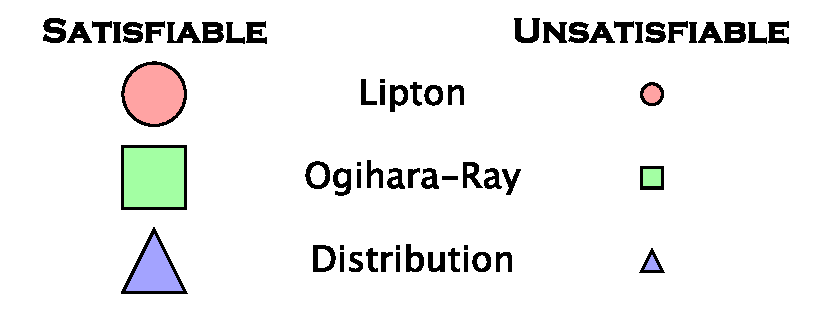
\includegraphics[width=0.7\textwidth]{./figures/key.pdf}

\caption{Key for output metrics.  Large shapes represent satisfiable instances and small shapes represent unsatisfiable instances.  Datapoints for Lipton's algorithm are represented with red circles, Ogihara and Ray's algorithm with green squares, and the Distribution algorithm with blue triangles. }
\label{metricKey}
\end{center}
\end{figure}
%%%%%%%%%%%%%%%%%%%%%%%%%%%%%%%%%

\FloatBarrier

%\subsection{Append}
%%%%%%%%%%%%%%%%%%%%%%%%%%%%%%%%%
\begin{figure}[htdp]

\reversemarginpar{
\textbf{Append} concatenates two oligonucleotides.  Figure \ref{appendFig} shows the number of appends for the naive implementations.  Figure \ref{appendFig_10} shows early termination on unsatisfiable $3$-CNF instances.   \\

The Distribution algorithm uses $O(k\cdot m)$ appends.  For unsatisfiable $k$-CNF input, the algorithm may terminate if there exist no witness candidates exist for the distribution of literals from remaining clauses. \\

Lipton's algorithm uses $\Theta(n)$ appends during the creation of a combinatorial space of $2^n$ witness candidates.\\

Ogihara and Ray's algoritm uses $O(n)$ appends.  Unsatisfiable $k$-CNF input may terminate once a conflict has been detected.\\
}

\begin{center}

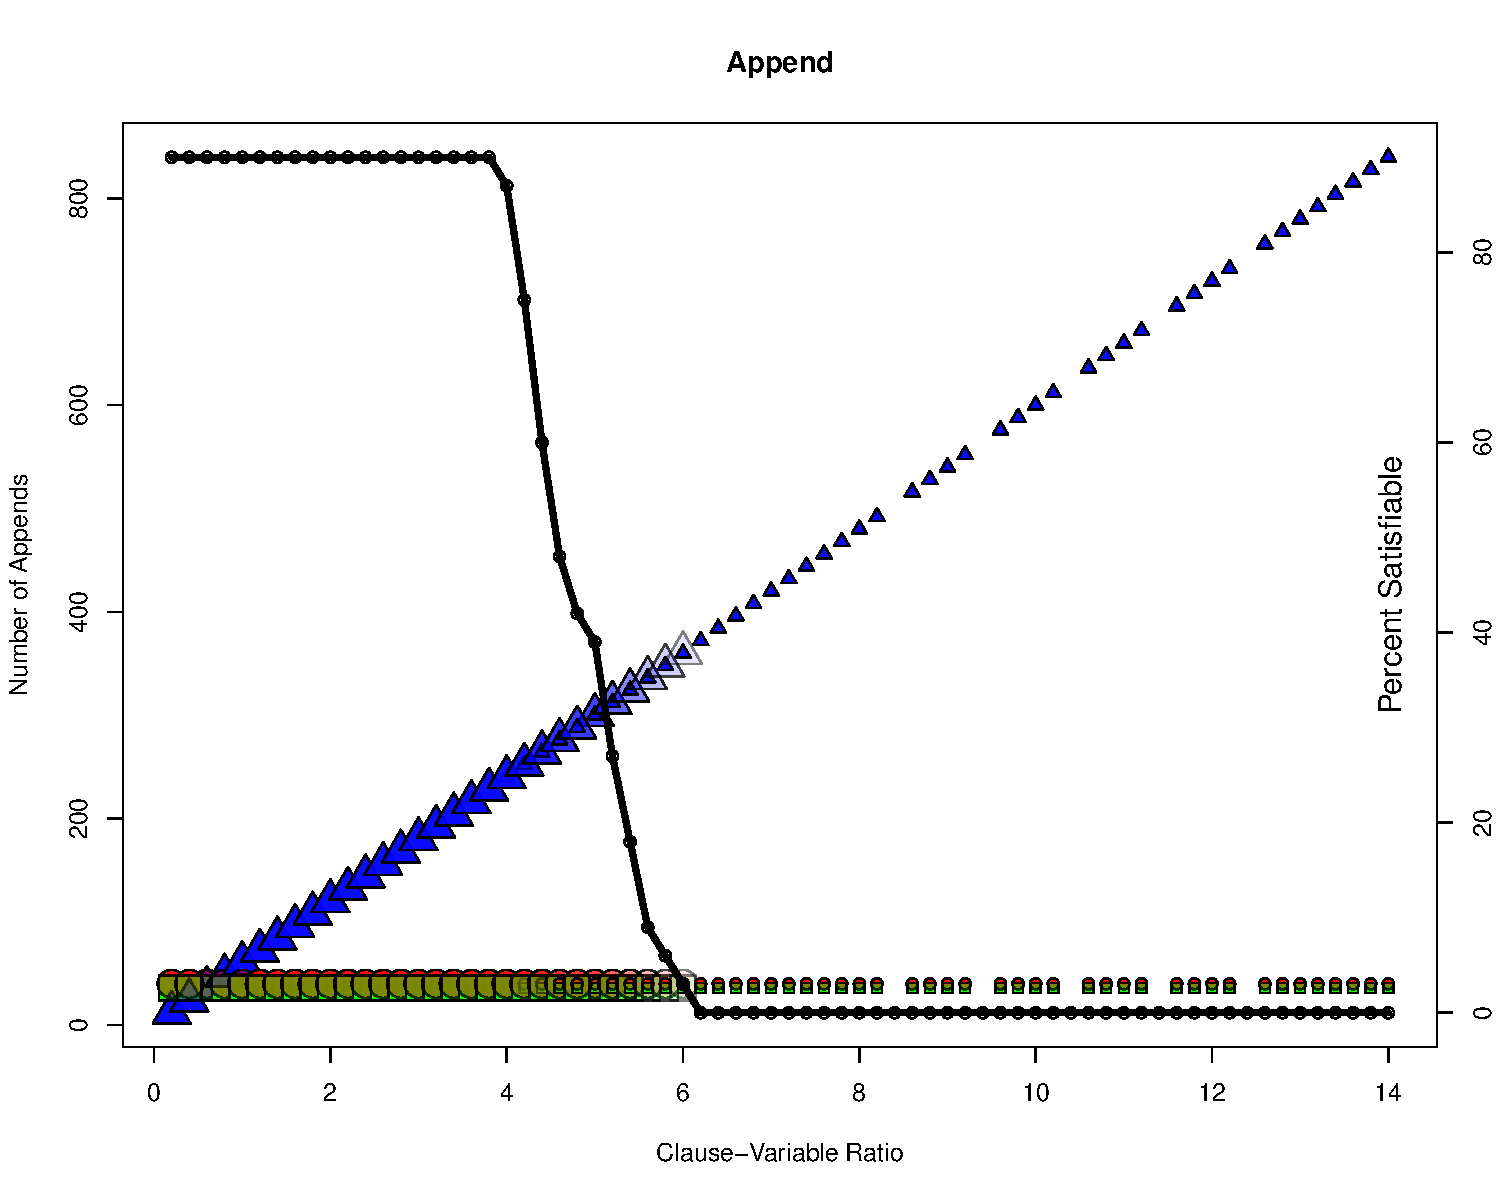
\includegraphics[width=1.1\textwidth]{./figures/metricOutput_n20/appendCount.pdf}

\caption{Clause to variable ratio $\alpha$ vs. Number of appends, with $n = 20$. }
\label{appendFig}
\end{center}
\end{figure}
%%%%%%%%%%%%%%%%%%%%%%%%%%%%%%%%%
\begin{figure}[htdp]

\begin{center}

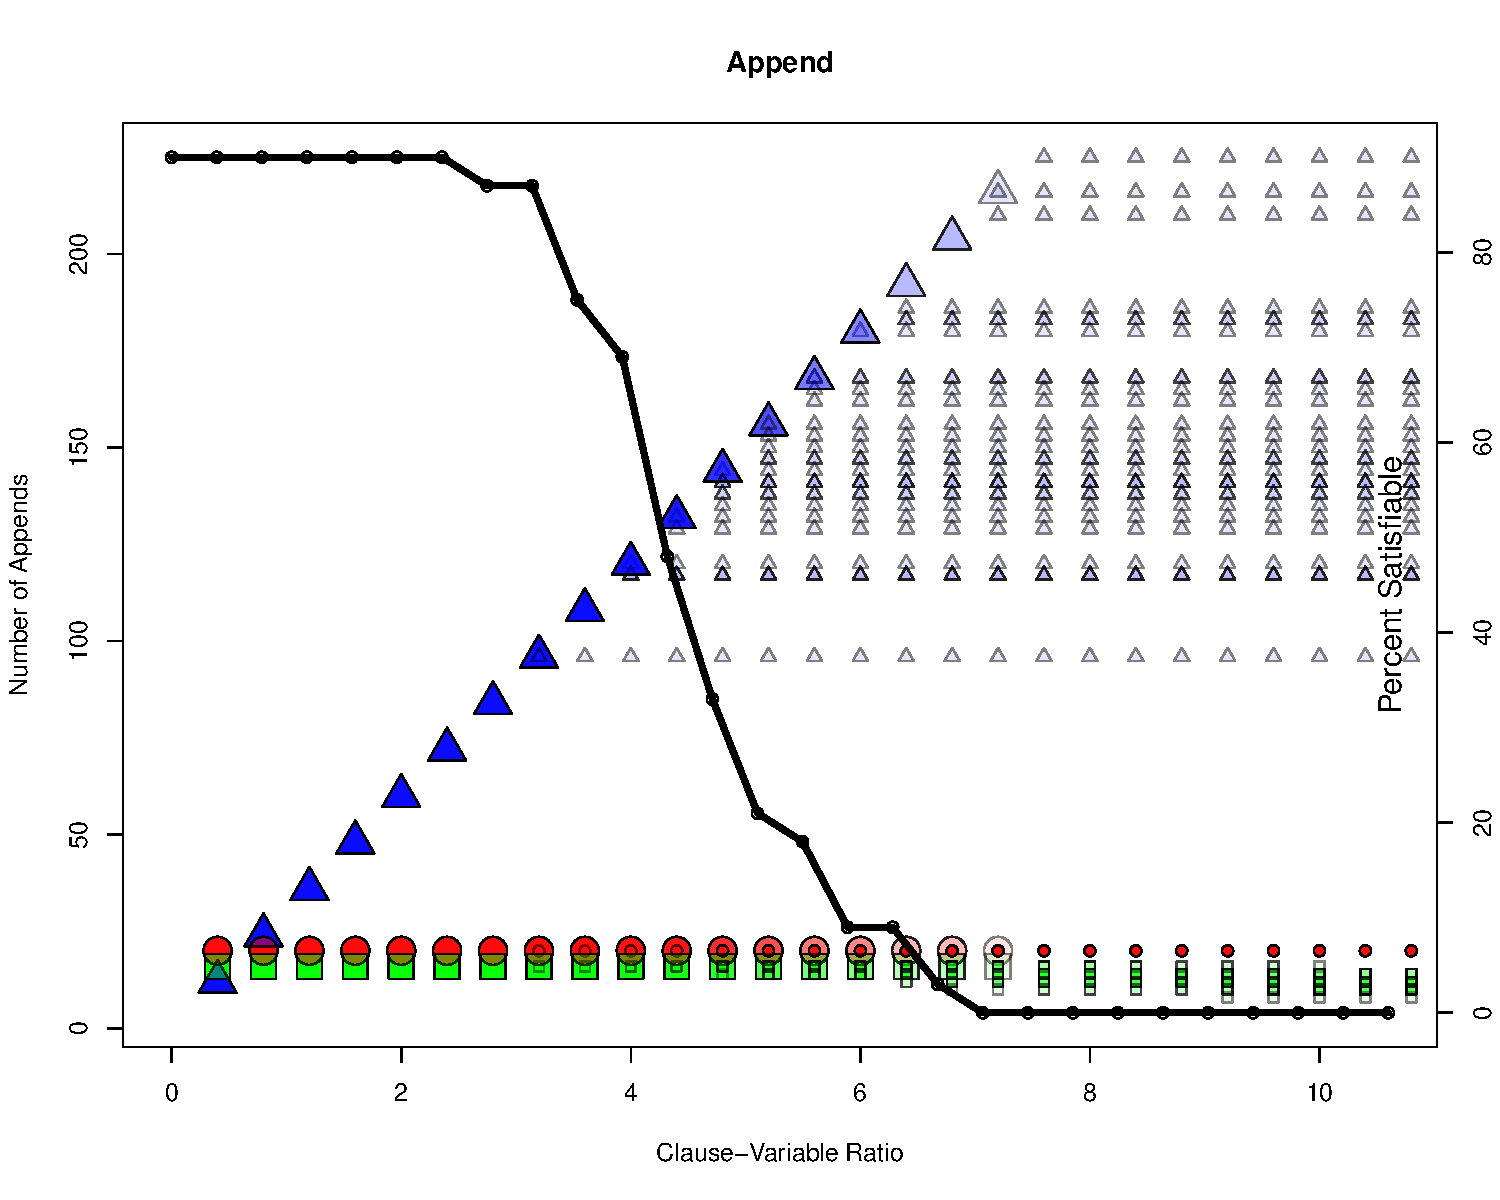
\includegraphics[width=1.1\textwidth]{./figures/metricOutput_n10/appendCount.pdf}

\caption{Clause to variable ratio $\alpha$ vs. Number of appends, with $n = 10$.  Algorithms terminate on detection of unsatisfiable input. }
\label{appendFig_10}
\end{center}
\end{figure}

%%%%%%%%%%%%%%%%%%%%%%%%%%%%%%%%%
\FloatBarrier
			
%\subsection{Extract}
%%%%%%%%%%%%%%%%%%%%%%%%%%%%%%%%%
\begin{figure}[htdp]

\reversemarginpar{

\textbf{Extract} filters oligonucleotides from a tube.  Figure \ref{extractFig} shows the number of extracts used in the naive implementations.  Figure \ref{extractFig_10} shows early termination on unsatisfiable $3$-CNF instances.   \\

Lipton's algorithm and the Distribution algorithm use $O(k\cdot m)$ extracts.  The Distribution algorithm varies a constant amount for maintaing the tubes $T_N$, $T_P$, and $T_V$.\\

Ogihara and Ray's algorithm uses $O(m)$ extracts.   Lipton's algorithm shares the same complexity from the experiments since we use $3$-CNF instances.\\

}

\begin{center}

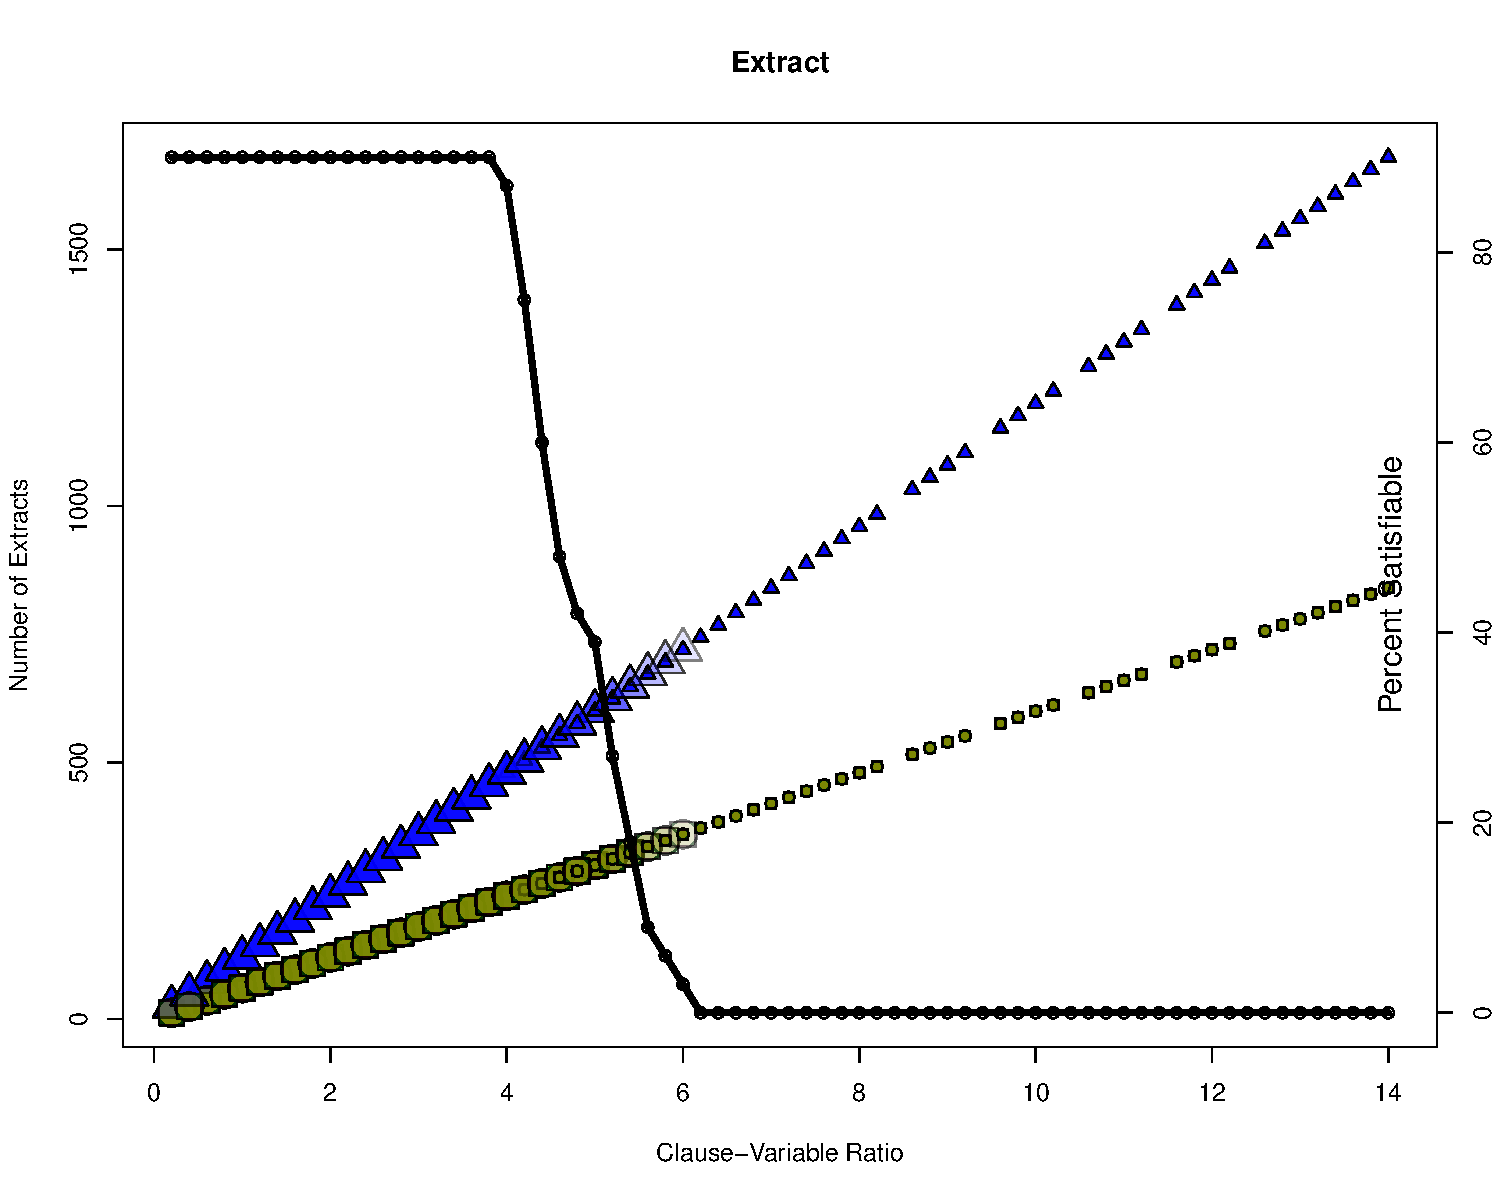
\includegraphics[width=1.1\textwidth]{./figures/metricOutput_n20/extractCount.pdf}

\caption{Clause to variable ratio $\alpha$ vs. Number of extracts, with $n= 20$. }
\label{extractFig}
\end{center}
\end{figure}
%%%%%%%%%%%%%%%%%%%%%%%%%%%%%%%%%
\FloatBarrier			
			
\begin{figure}[htdp]

\begin{center}

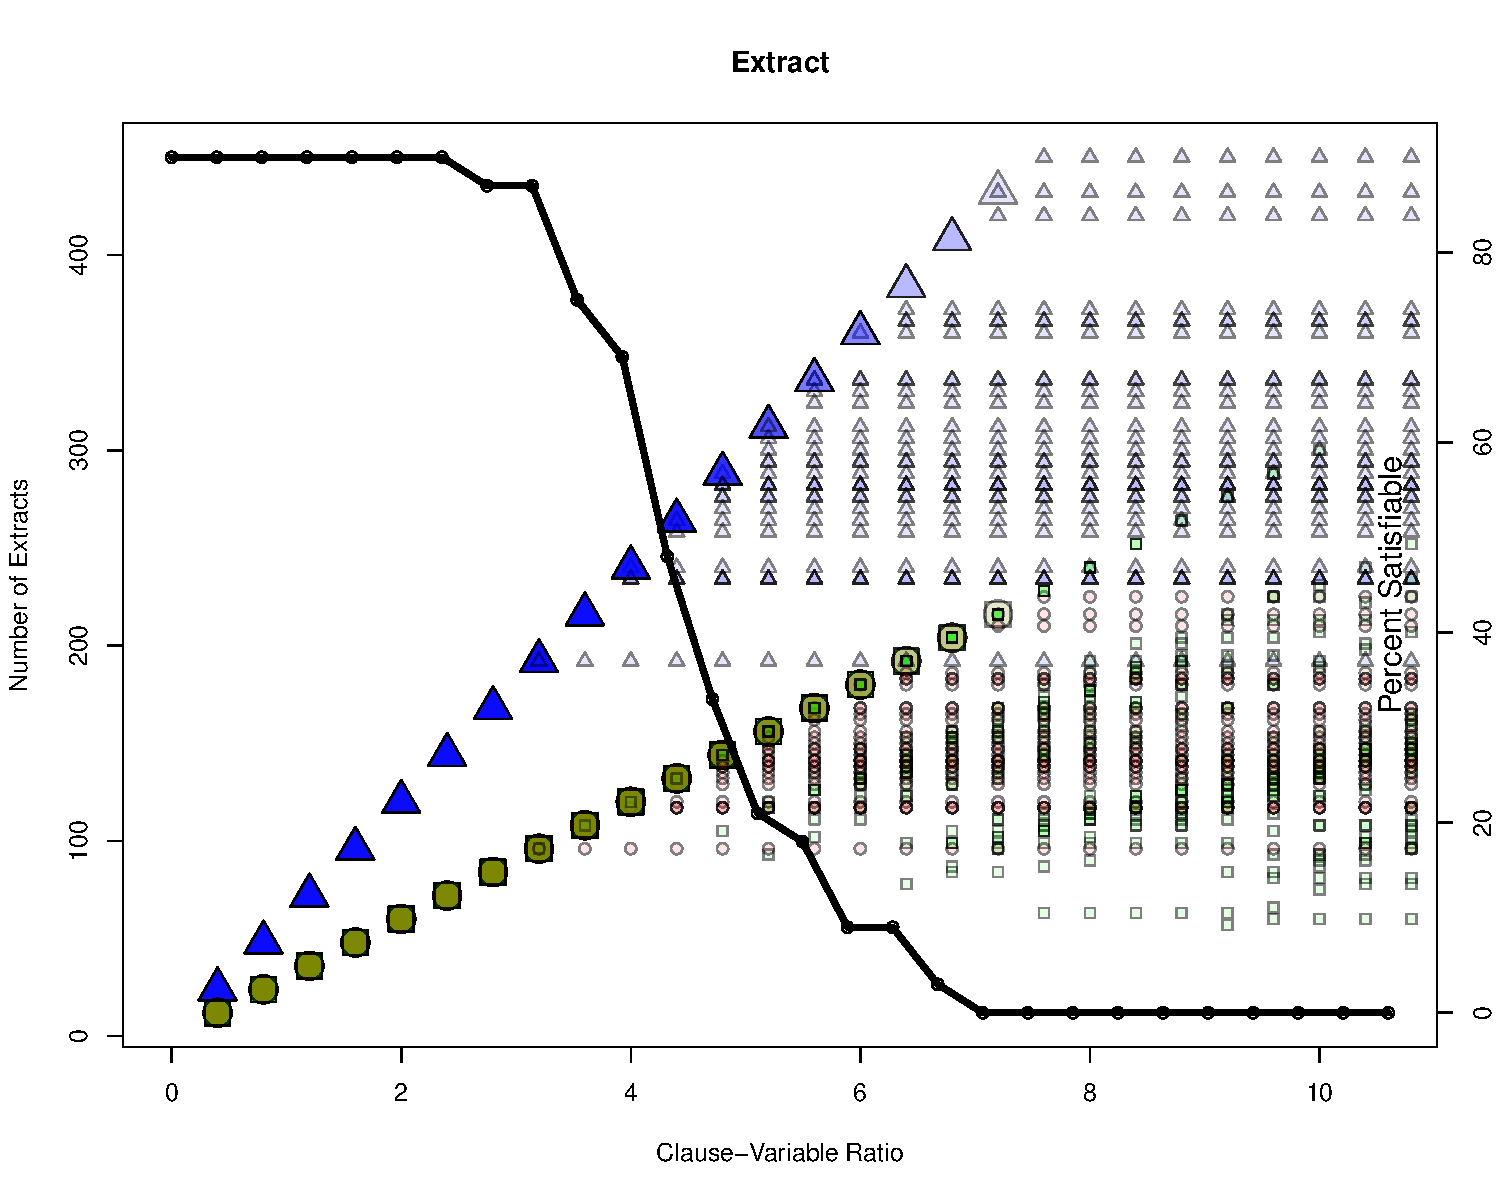
\includegraphics[width=1.1\textwidth]{./figures/metricOutput_n10/extractCount.pdf}

\caption{Clause to variable ratio $\alpha$ vs. Number of extracts, with $n = 10$.  Algorithms terminate on detection of unsatisfiable input. }
\label{extractFig_10}
\end{center}
\end{figure}

%%%%%%%%%%%%%%%%%%%%%%%%%%%%%%%%%			
			
%\subsection{Mix}
%%%%%%%%%%%%%%%%%%%%%%%%%%%%%%%%%
\begin{figure}[htdp]

\reversemarginpar{
		\textbf{Mix} combines the contents of $n$ tubes into a storage tube.  Figure \ref{mixFig} shows the number of mixes used in the naive implementations.  Figure \ref{mixFig_10} shows early termination on unsatisfiable $3$-CNF instances. \\
		
		Lipton's algorithm uses $\Theta(m(k+1)+n)$ mix operations for satisfiable $k$-CNF instances.  This includes preparing a combinatorial space with the {\sc Combinatorial Generate} subroutine.  \\
		
		The Distribution algorithm uses $O(k\cdot m)$ mixes for distributing each clause with $k$ literals into a set of witnesses satisfying each clause.  This set of witnesses get mixed into the tube satisfying all distributed clauses.\\
		
		Ogihara and Ray's algorithm expands on clauses matching in the third ordered literal.  The algorithm uses $O(m+n)$ mixes.  This includes a maximum of $m$ mixes for each clause, and $n$ mixes for extending witnesses for $\phi$.  \\

}

\begin{center}

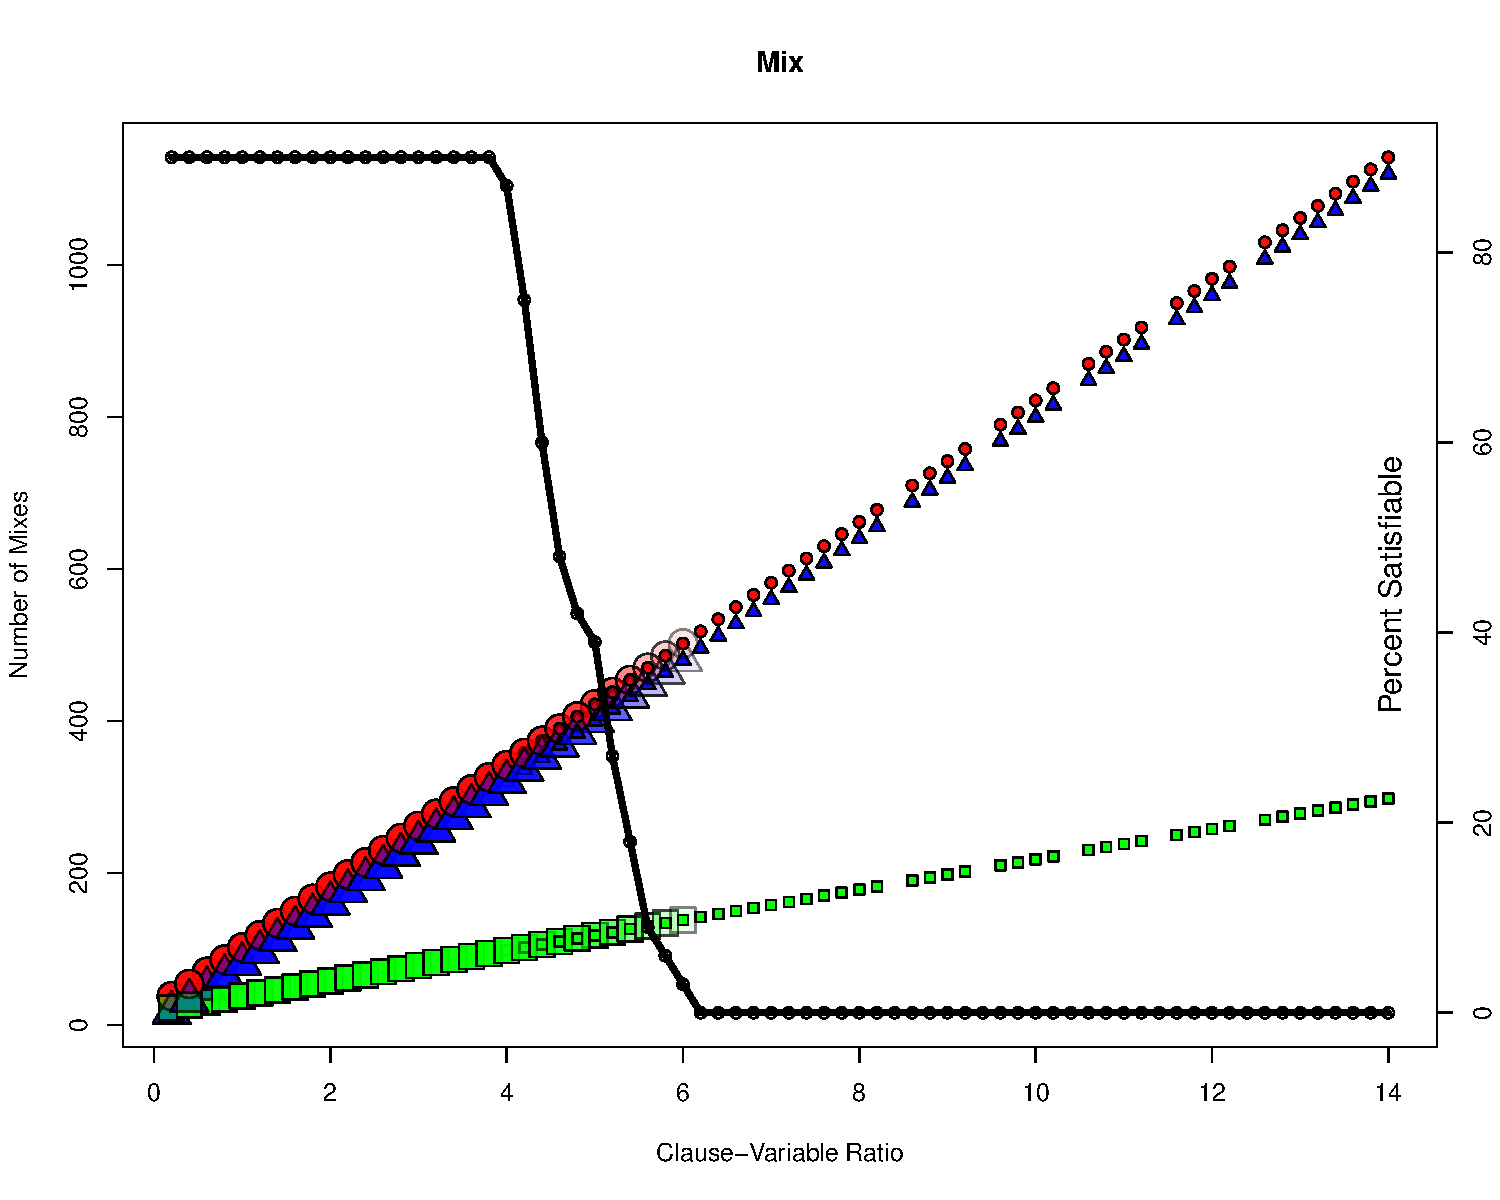
\includegraphics[width=1.1\textwidth]{./figures/metricOutput_n20/mixCount.pdf}

\caption{Clause to variable ratio $\alpha$ vs. Number of mixes, with $n = 20$.}
\label{mixFig}
\end{center}
\end{figure}

%%%%%%%%%%%%%%%%%%%%%%%%%%%%%%%%%
\begin{figure}[htdp]

\begin{center}

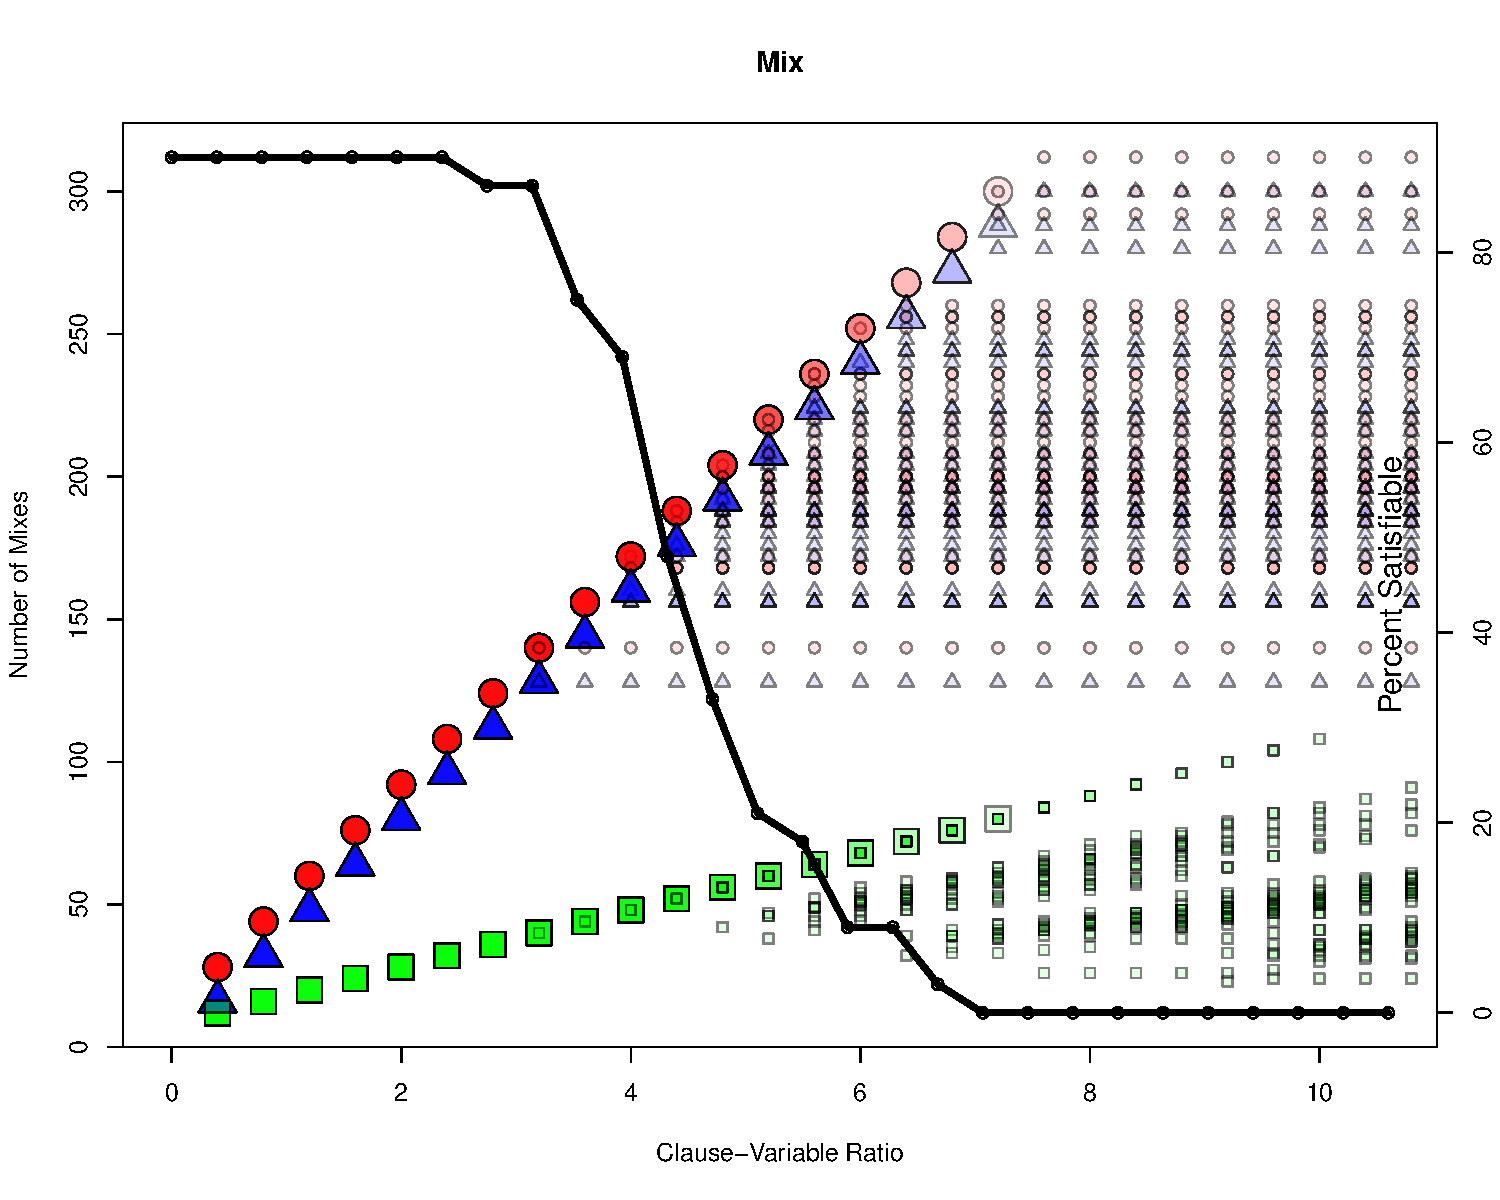
\includegraphics[width=1.1\textwidth]{./figures/metricOutput_n10/mixCount.pdf}

\caption{Clause to variable ratio $\alpha$ vs. Number of mixes, with $n = 10$.  Algorithms terminate on detection of unsatisfiable input. }
\label{mixFig_10}
\end{center}
\end{figure}

%%%%%%%%%%%%%%%%%%%%%%%%%%%%%%%%%
\FloatBarrier

%\subsection{Purify}
%%%%%%%%%%%%%%%%%%%%%%%%%%%%%%%%%
\begin{figure}[htdp]

\reversemarginpar{
\textbf{Purify} ensures a uniform distribution of each independent oligonucleotide in a tube.  Figure \ref{purifyFig} shows the number of purifications used in the naive implementations.  Figure \ref{purifyFig_10} shows early termination on unsatisfiable $3$-CNF instances. \\

Ogihara and Ray's algorithm requires $O(m+n)$ purifications.  The algorithm requires a purification for each of the $m$ clauses, and a purification for each of the $n$ variables. \\

Lipton's and the Distribution algorithms each use $O(m)$ purifications.  Each of these algorithms purify the contents on the iteration of each of the $m$ clauses.

 }

\begin{center}

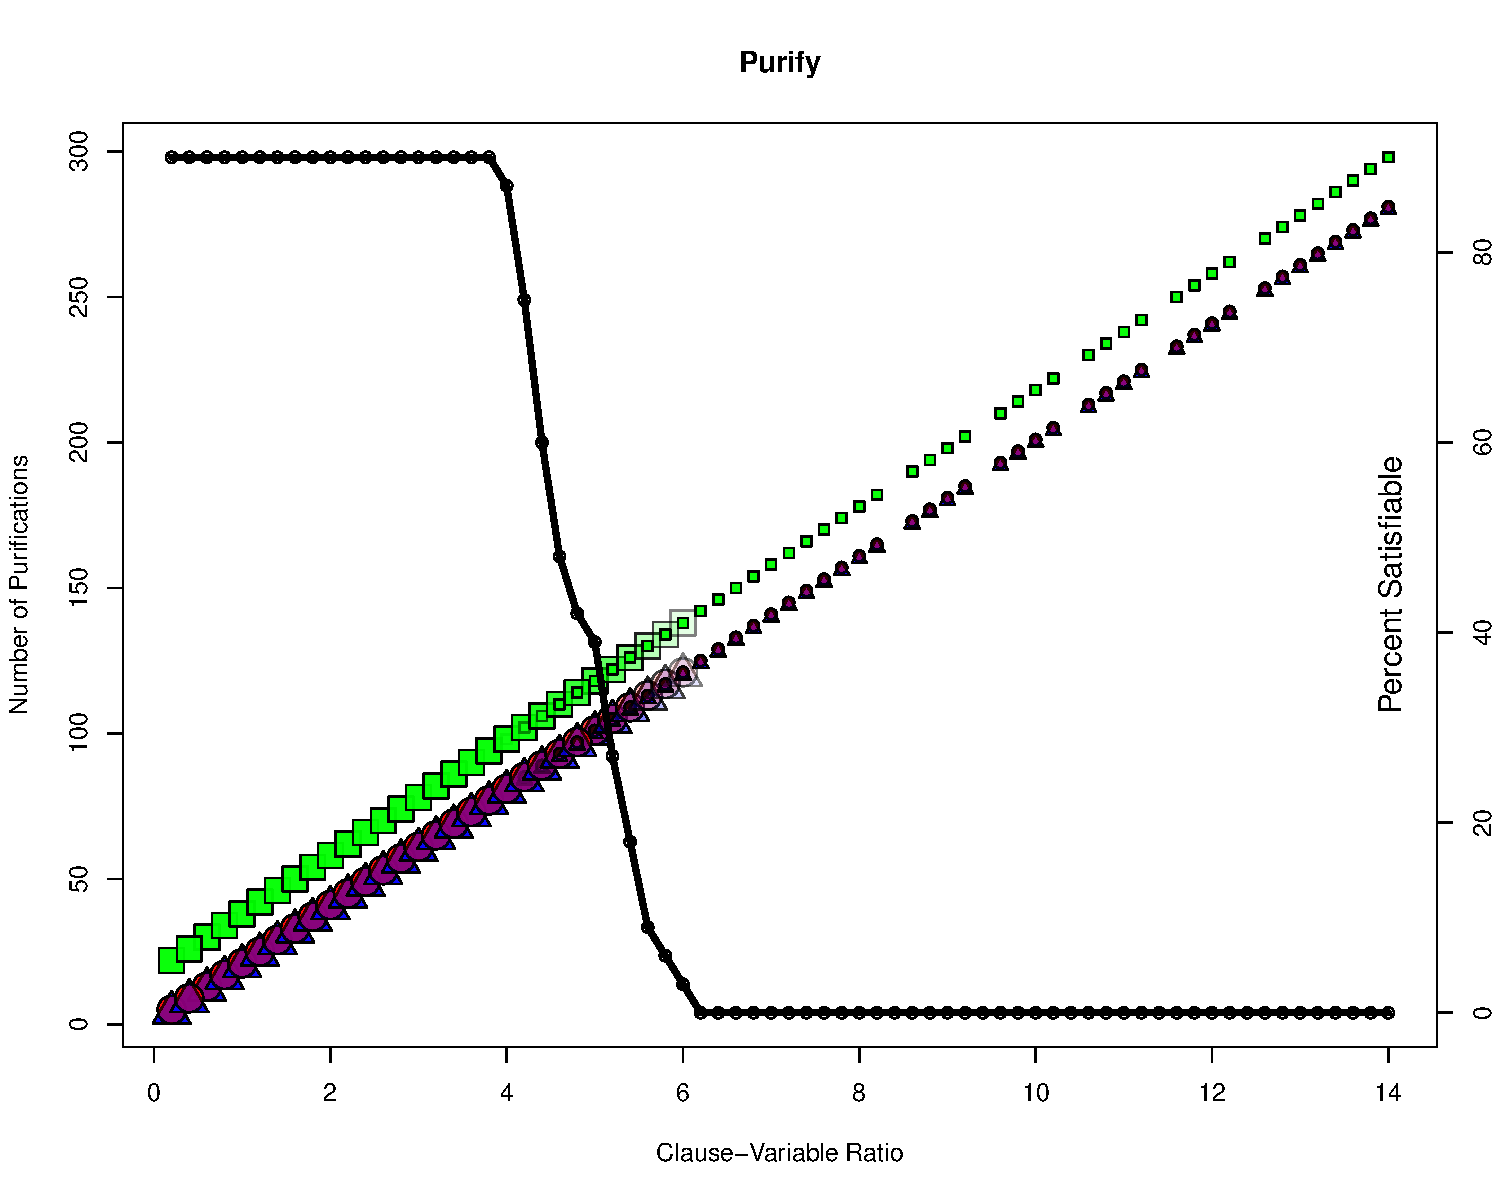
\includegraphics[width=1.1\textwidth]{./figures/metricOutput_n20/purifyCount.pdf}

\caption{Clause to variable ratio $\alpha$ vs. Number of purifications, with $n = 20$. }
\label{purifyFig}
\end{center}
\end{figure}
%%%%%%%%%%%%%%%%%%%%%%%%%%%%%%%%%

\begin{figure}[htdp]

\begin{center}

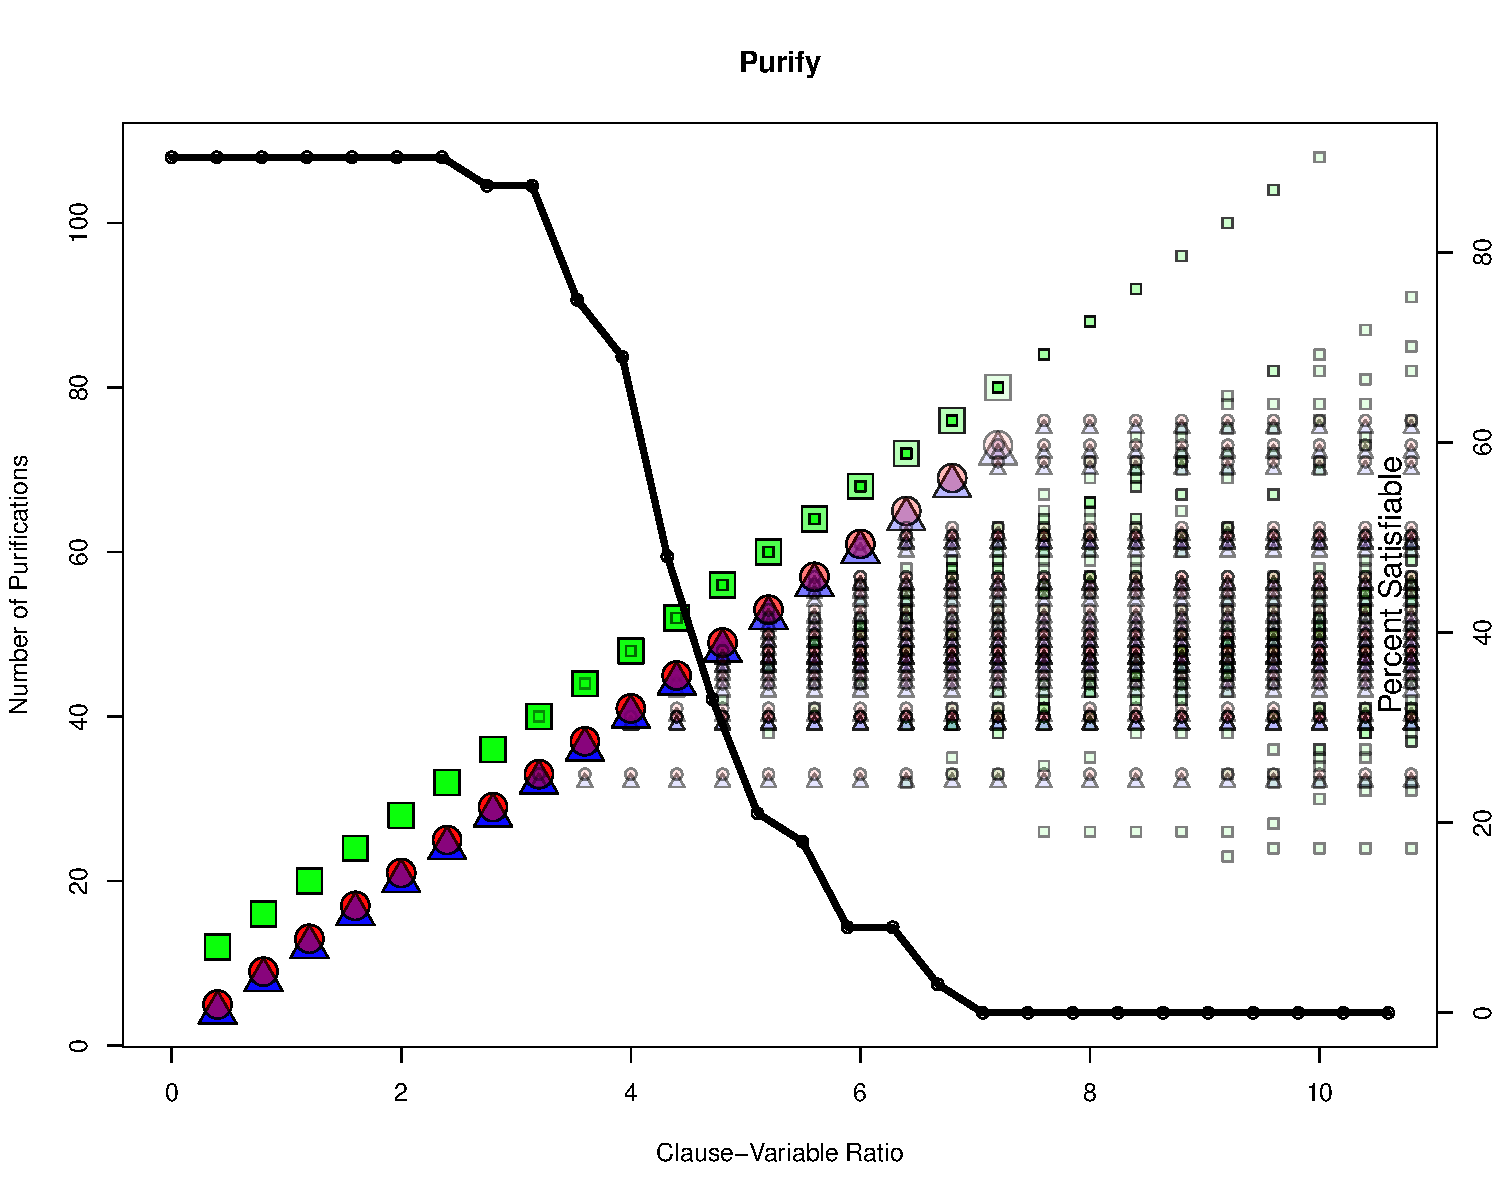
\includegraphics[width=1.1\textwidth]{./figures/metricOutput_n10/purifyCount.pdf}

\caption{Clause to variable ratio $\alpha$ vs. Number of purifications, with $n = 10$.  Algorithms terminate on detection of unsatisfiable input. }
\label{purifyFig_10}
\end{center}
\end{figure}

%%%%%%%%%%%%%%%%%%%%%%%%%%%%%%%%%
\FloatBarrier


%\subsection{Split}
%%%%%%%%%%%%%%%%%%%%%%%%%%%%%%%%%
\begin{figure}[htdp]

\reversemarginpar{

\textbf{Split} portions a tube into two exact tubes.  Figure \ref{splitFig} shows the number of splits used in the naive implementations.  Figure \ref{splitFig_10} shows early termination on unsatisfiable $3$-CNF instances. \\

The Distribution algorithm uses $O(k \cdot m)$ splits.  The split operation occurs on each of the $m$ clauses of a $k$-CNF instance.\\

Lipton's algorithm uses $\Theta(n)$ splits during the creation of a combinatorial space of $2^n$ witness candidates with {\sc Combinatorial Generate}.\\

Ogihara and Ray's algorithm uses $O(n)$ splits.  The algorithm requires a copy of witness candidates in the tubes ($T_P$ and $T_N$).  The tubes $T_P$ and $T_N$ extend with positive and negative literal assignments. 

 }

\begin{center}

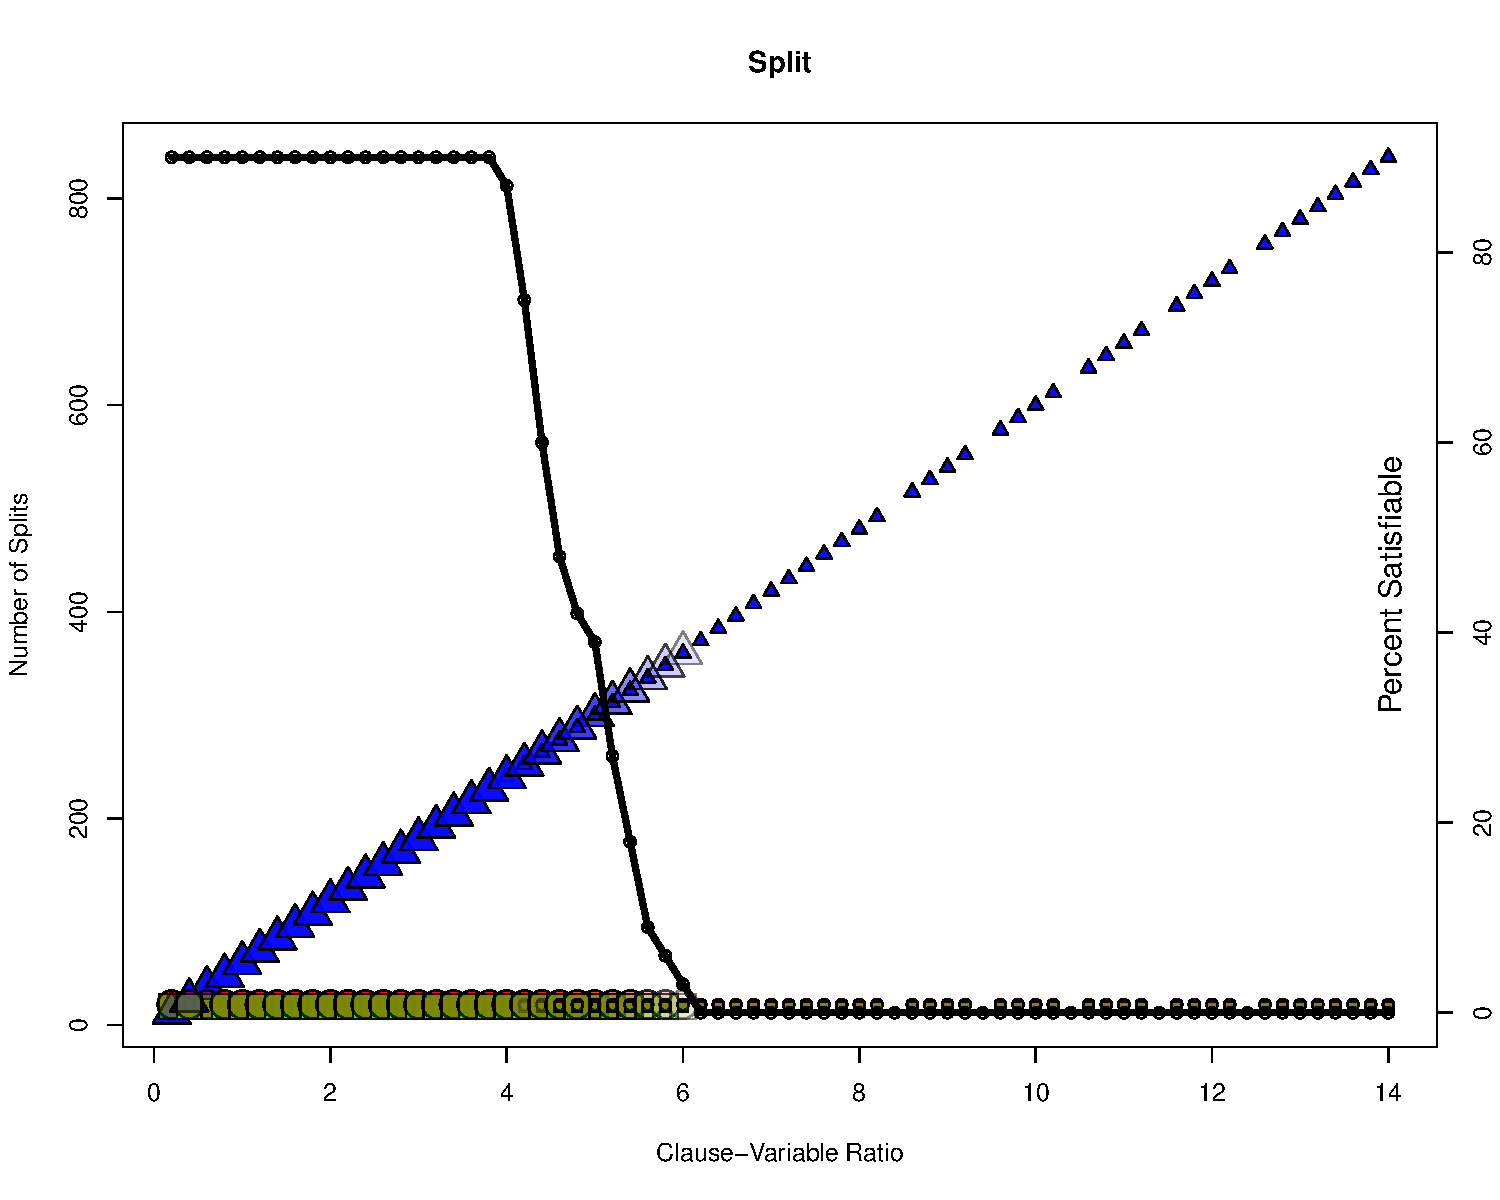
\includegraphics[width=1.1\textwidth]{./figures/metricOutput_n20/splitCount.pdf}

\caption{Clause to variable ratio $\alpha$ vs. Number of splits, with $n = 20$. }
\label{splitFig}
\end{center}
\end{figure}
%%%%%%%%%%%%%%%%%%%%%%%%%%%%%%%%%
\begin{figure}[htdp]

\begin{center}

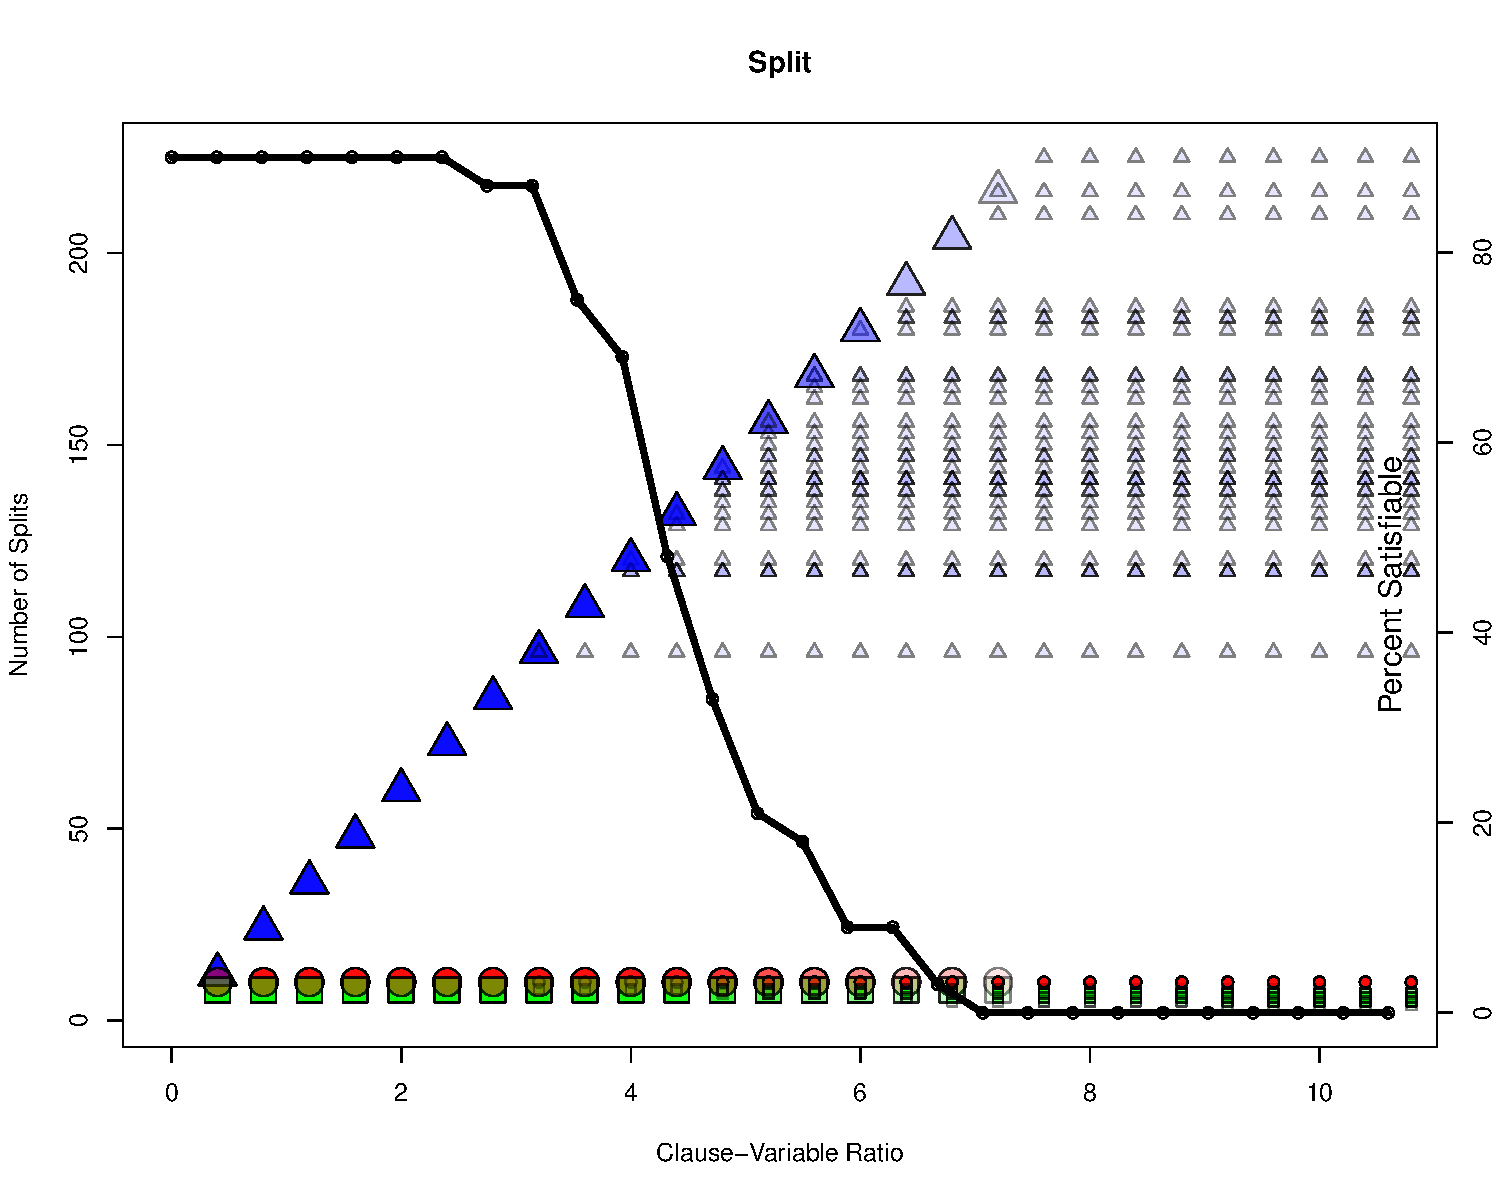
\includegraphics[width=1.1\textwidth]{./figures/metricOutput_n10/splitCount.pdf}

\caption{Clause to variable ratio $\alpha$ vs. Number of splits, with $n = 10$.  Algorithms terminate on detection of unsatisfiable input. }
\label{splitFig_10}
\end{center}
\end{figure}

%%%%%%%%%%%%%%%%%%%%%%%%%%%%%%%%%

\FloatBarrier

			
%\subsection{Time}
%%%%%%%%%%%%%%%%%%%%%%%%%%%%%%%%%
\begin{figure}[htdp]

\reversemarginpar{
\textbf{Time} measures algorithm execution time in seconds.  Figure \ref{timeFig} shows the execution time in seconds used in the naive implementations.  Figure \ref{timeFig_10} shows early termination on unsatisfiable $3$-CNF instances. \\

Ogihara and Ray's algorithm requires the least amount of time.  The algorithm takes the greatest amount of time for under-constrained instances (causing a large number of witnesses to be generated).   Less pruning occurs in over-constrained instances, reducing the execution time of test instances.\\

Lipton's algorithm executes in exponential time $\alpha \approx [4.0, 6.0]$ (the phase transition region for 3-{\sc Sat}) taking the longest.\\

The Distribution algorithm executes in exponential time, and performs better than Lipton's algorithm for low conflict ratios.  Instances take the longest from $\alpha \approx [4.0, 6.0]$ (in the $3$-{\sc Sat} phase-transition region).
}

\begin{center}

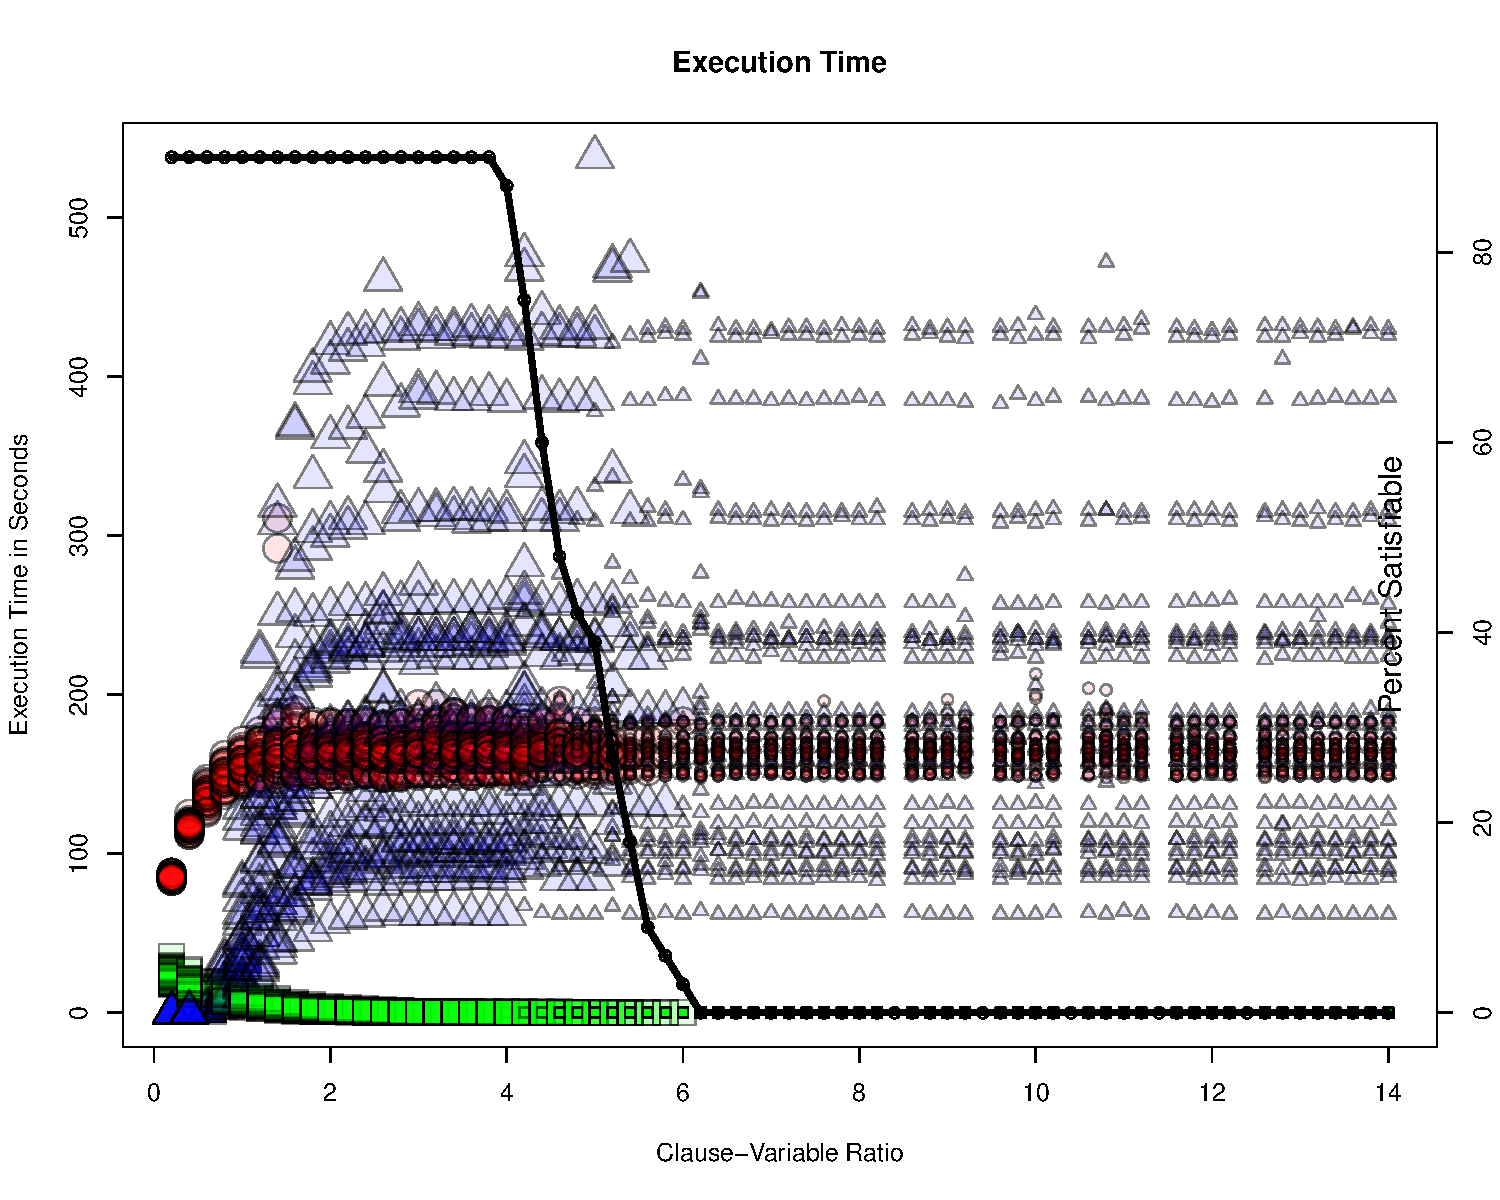
\includegraphics[width=1.1\textwidth]{./figures/metricOutput_n20/executionTime.pdf}

\caption{Clause to variable ratio $\alpha$ vs. execution time in seconds, with $n = 20$. }
\label{timeFig}
\end{center}
\end{figure}

%%%%%%%%%%%%%%%%%%%%%%%%%%%%%%%%%
\begin{figure}[htdp]

\begin{center}

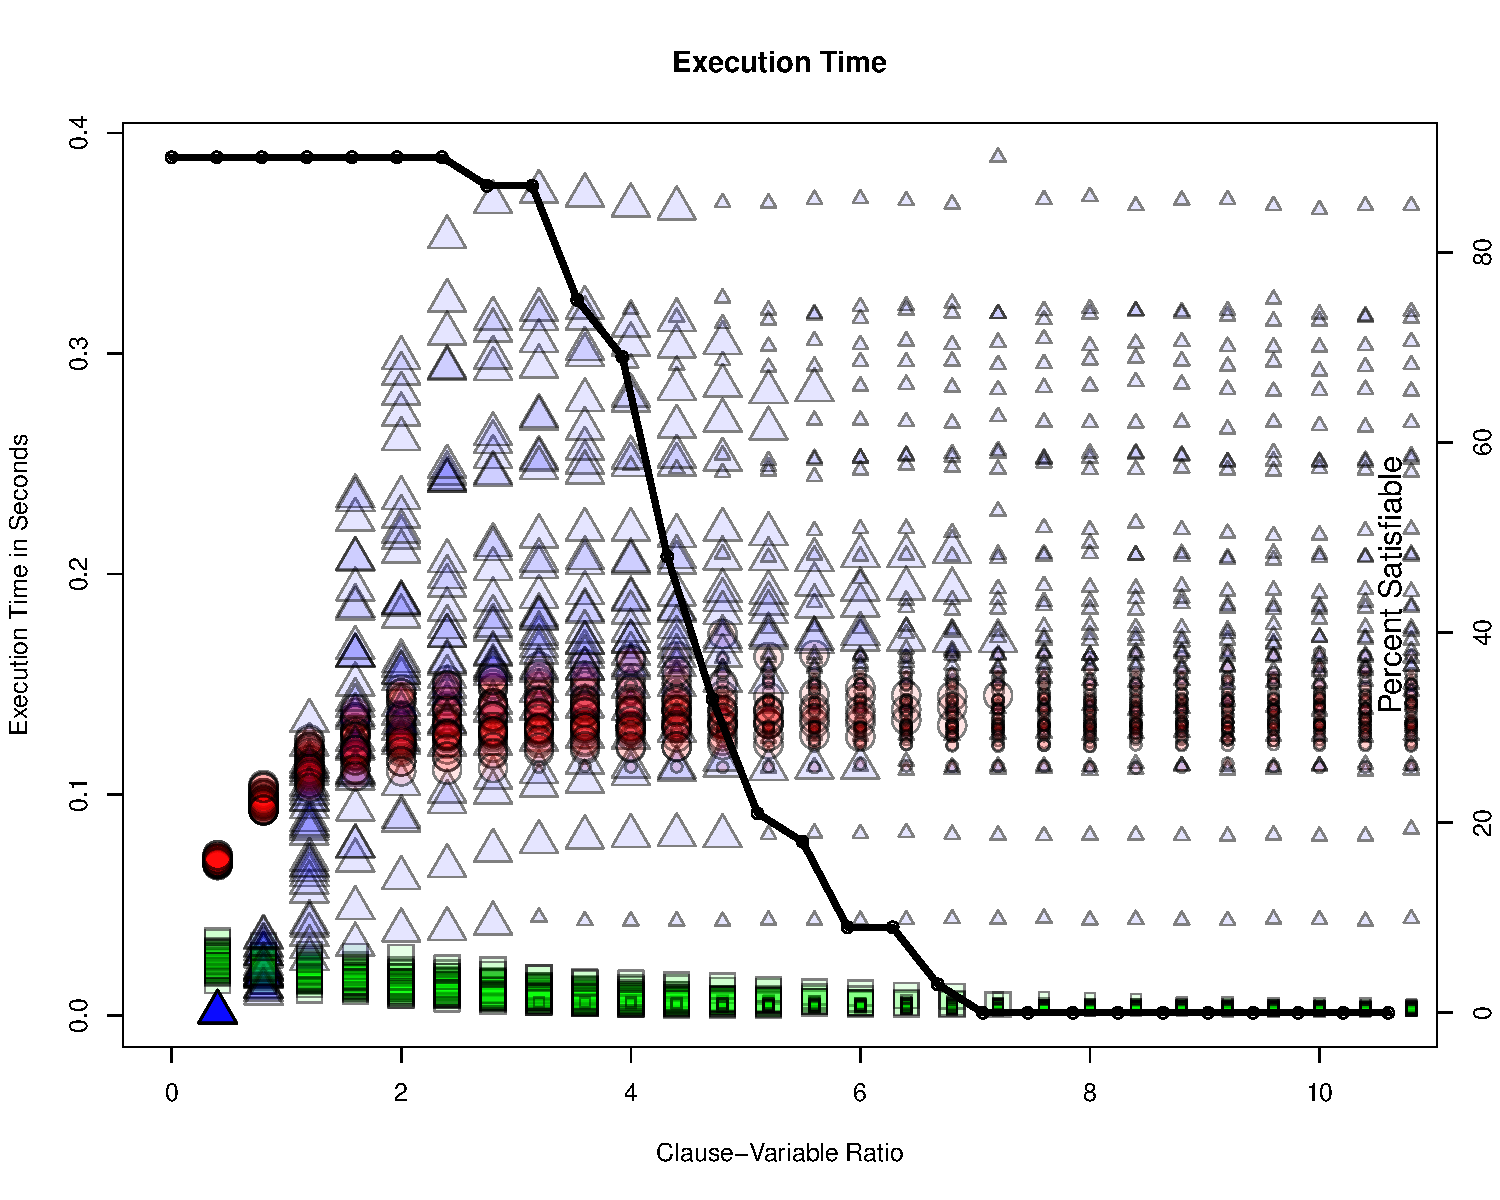
\includegraphics[width=1.1\textwidth]{./figures/metricOutput_n10/executionTime.pdf}

\caption{Clause to variable ratio $\alpha$ vs. Number of splits, with $n = 10$.  Algorithms terminate on detection of unsatisfiable input. }
\label{timeFig_10}
\end{center}
\end{figure}

%%%%%%%%%%%%%%%%%%%%%%%%%%%%%%%%%
\FloatBarrier
			
%\subsection{Solution space}
%%%%%%%%%%%%%%%%%%%%%%%%%%%%%%%%%
\begin{figure}[htdp]

\reversemarginpar{
\textbf{Memory} measures witness footprint in Bytes.  Figure \ref{memoryFig} shows the satisfiable instance witness memory.  Figure \ref{memoryFigDetail} shows a detailed view of Figure \ref{memoryFig} from $\alpha = [3,6]$.\\

Lipton's and Ogihara and Ray's algorithms share the same solution footprint.\\

The Distribution algorithm contains a larger solution footprint after the trivially satisfiable instances with $\alpha \approx [0.2, 1.0)$.  The space contains a set of over-constrained assignments from $\alpha \approx [1.0, 4.0]$.  \\

Each {\sc Satisfiability} instance has a constrained solution space during the phase-transition region.  We scale the axis in Figure \ref{memoryFig} to observe only satisfiable instances.
}

\begin{center}

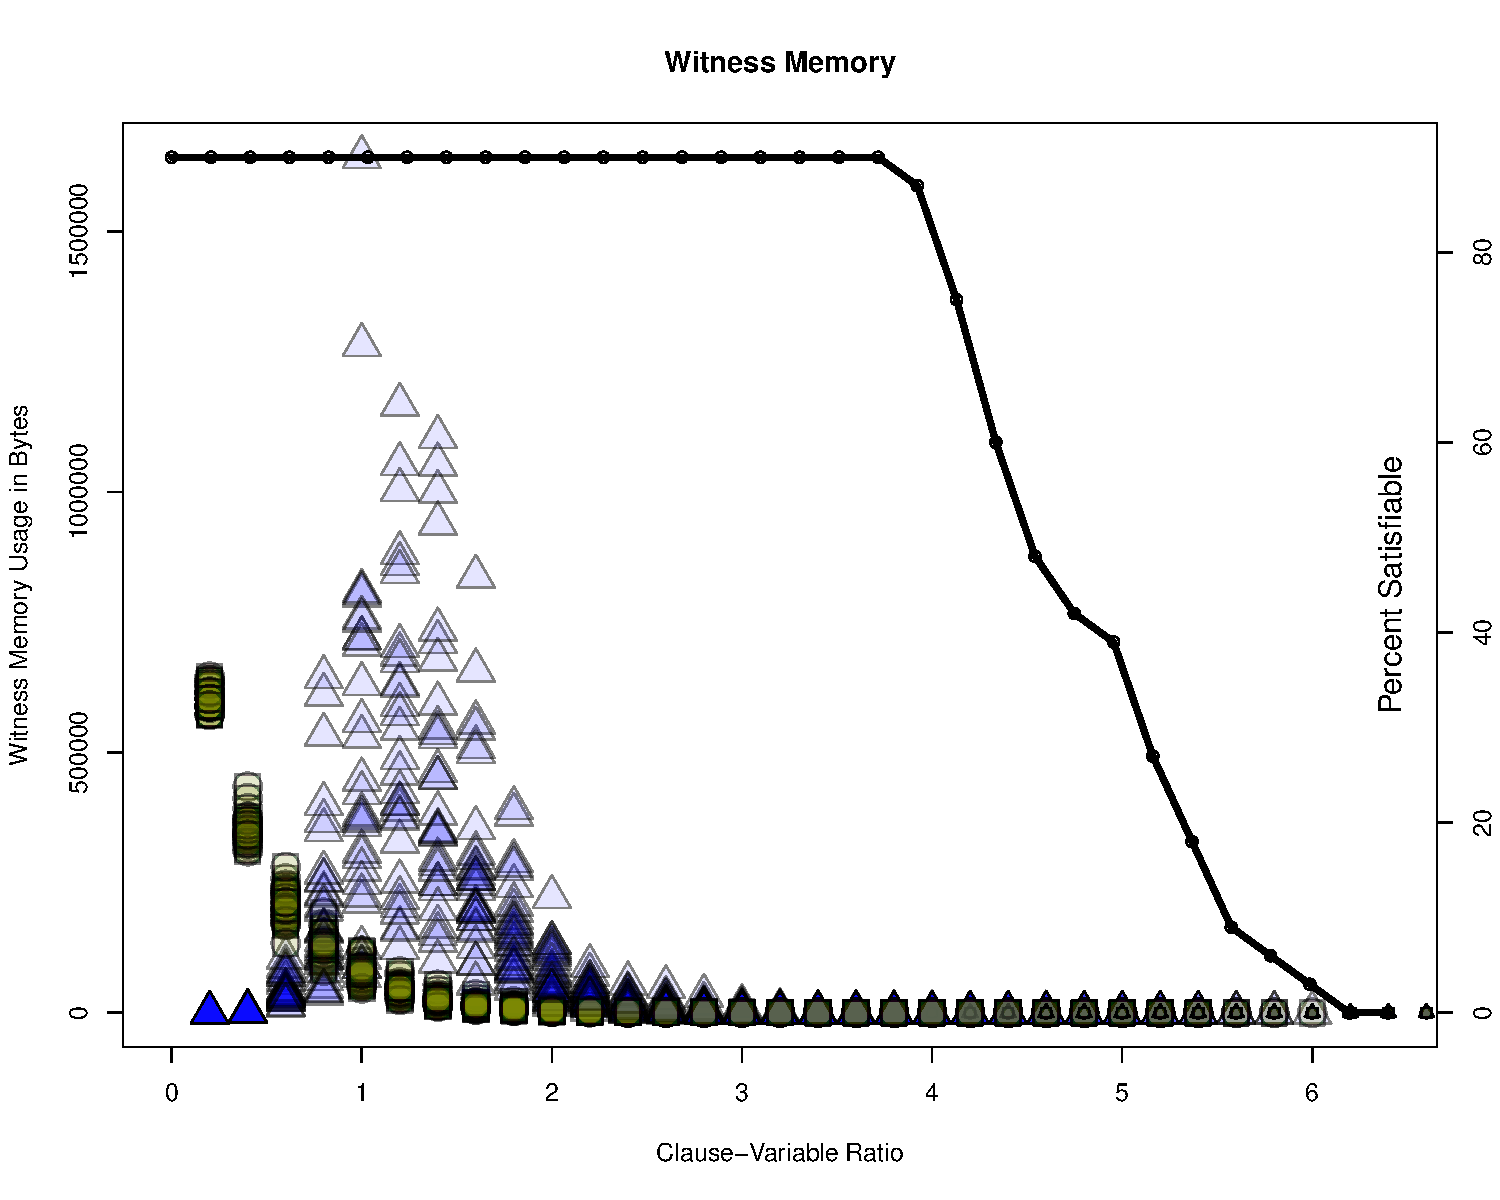
\includegraphics[width=1.1\textwidth]{./figures/plotImage/memory0-6_2.pdf}

\caption{Clause to variable ratio $\alpha$ vs. satisfiable solution footprint in Bytes, with $n = 20$. }
\label{memoryFig}
\end{center}
\end{figure}


\begin{figure}[htdp]
\begin{center}

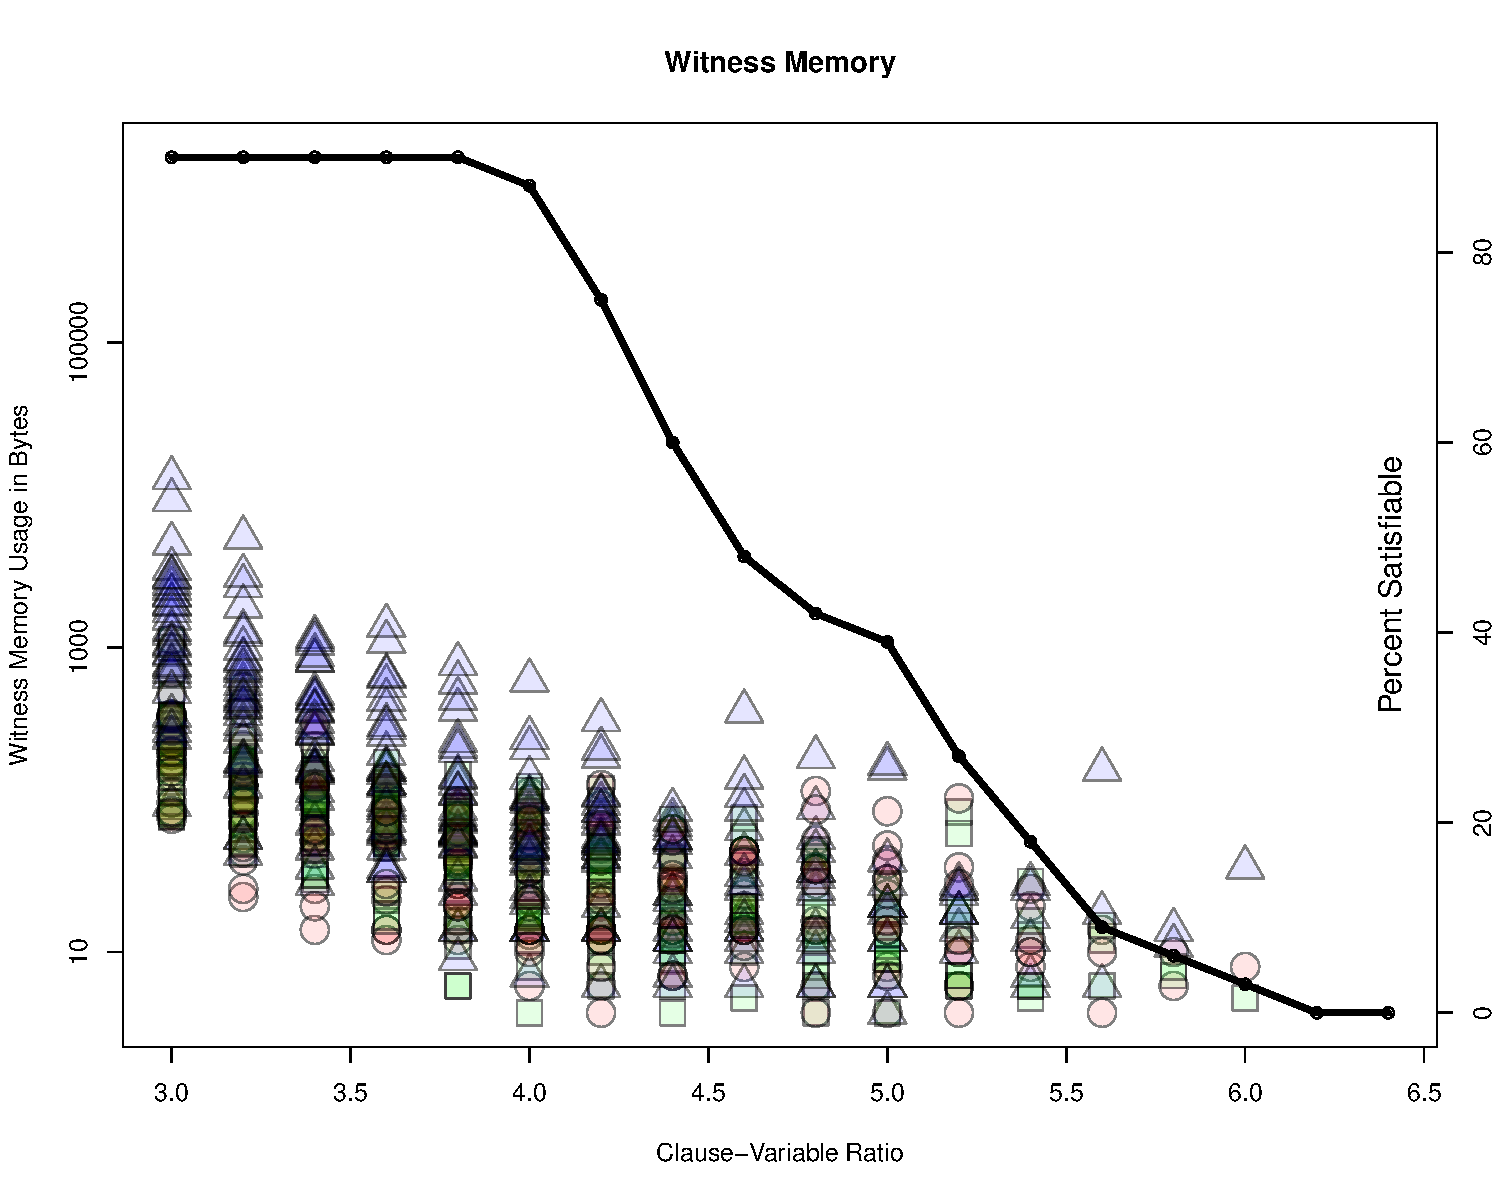
\includegraphics[width=1.1\textwidth]{./figures/plotImage/memory3-6_2.pdf}

\caption{Detailed view of Figure \ref{memoryFig} from $\alpha = [3,6]$. }
\label{memoryFigDetail}
\end{center}
\end{figure}

%%%%%%%%%%%%%%%%%%%%%%%%%%%%%%%%%

\FloatBarrier

	\section{Summary of Molecular Algorithms}

		Table \ref{timeComplexityMolecularOperators} shows a comparison of the molecular operators of the algorithms under test.  Once the solution space $T_S = \emptyset$ the algorithms can terminate.  This provides the upper bounds for execution of various $k$-CNF instances.  
		
		\begin{table}[htdp]
				\caption{Time complexity of molecular operators for each of the molecular algorithms.}
				\begin{center}
				\begin{tabular}{|c|c|c|c|c|}
					\hline
					\textbf{ Operator} & {\sc Combinatorial Generate} & {\sc Lipton}           & {\sc Ogihara-Ray}  & {\sc Distribution} \\ \hline
					mix	               & $\Theta(n)$                  & $O(k\cdot m + m)$      & $O(m + n)$         & $O(k\cdot m + m)$ \\
					extract            & ---                          & $O(k\cdot m)$          & $O(m)$             & $O(k\cdot m)$ \\
					split	           & $\Theta(n)$                  & ---                    & $O(n)$             & $O(k\cdot m)$ \\
					purify	           & $\Theta(1)$                  & $O(m)$                 & $O(m + n)$         & $O(m)$ \\
					append	           & $\Theta(n)$                  & ---                    & $O(n)$             & $O(k\cdot m)$ \\
					\hline
				\end{tabular}
				\end{center}
				\label{timeComplexityMolecularOperators}
				\end{table}%
		
			\FloatBarrier		
		
		




		
	

\input{ch8_Conclusions.tex}

\newpage
\addcontentsline{toc}{chapter}{Bibliography} 
\bibliographystyle{acm}
\bibliography{./refAll}

\appendix

\chapter{Source}

\section{Contributed}

\noindent Download Molecular Simulation:

\begin{itemize}
	\item \url{https://github.com/dncarley/MolecularSimulation}
\end{itemize}
\begin{itemize}
\item Documentation
	\begin{itemize}
		\item Online Documentation:
			\begin{itemize}
				\item \url{http://www.cs.rit.edu/~dnc6813/project/generatedDocs/index.html}
			\end{itemize}
		\item Offline Documentation:
		\begin{itemize}
			\item \url{http://www.cs.rit.edu/~dnc6813/project/refman.pdf}
		\end{itemize}
	\end{itemize}
\end{itemize}


\noindent Download {\sc Sat} Datapoints Visualization:
\begin{itemize}
	\item \url{https://github.com/dncarley/VisualizeSatDatapoints}
\end{itemize}

%\noindent Interact with online datapoints at:
%
%\url{http://www.cs.rit.edu/~dnc6813/project/applet_js/index.html}

\section{External}

\noindent Download David Wilson's $k$-{\sc Sat} Generator:

\begin{itemize}
	\item \url{http://research.microsoft.com/en-us/um/people/dbwilson/ksat/default.htm}
\end{itemize}

\noindent Download Doxygen:

\begin{itemize}
	\item \url{http://www.stack.nl/~dimitri/doxygen/}
\end{itemize}

\noindent Download Ben Fry's examples for \textit{Visualizing Data}:

\begin{itemize}
	\item \url{http://benfry.com/writing/archives/3}
\end{itemize}



\chapter{Molecular algorithm trace}

\section{Example {\sc Satisfiability} instance}


\[
 \phi = (x_1 \vee x_2 \vee \neg x_3) \wedge  (x_2 \vee x_3 \vee \neg x_4) \wedge (\neg x_1 \vee \neg x_3 \vee \neg x_4)
\]


\section{Lipton's Algorithm}

\[
T  = \text{{\sc Combinatorial Generate}}(4)
\]

\[
T = 
\]
\begin{verbatim}
	STTTT SFTTT STFTT SFFTT STTFT SFTFT STFFT SFFFT
	STTTF SFTTF STFTF SFFTF STTFF SFTFF STFFF SFFFF
\end{verbatim}
	
Next select Clause 1:

\[
C_1 = (x_1 \vee x_2 \vee \neg x_3)
\]

\begin{verbatim}
	STTTT SFTTT STFTT SFFTT STTFT SFTFT STFFT SFFFT
	STTTF SFTTF STFTF SFFTF STTFF SFTFF STFFF SFFFF
\end{verbatim}
	
	Extract $x_1$:

\begin{verbatim}
		STTTT      STFTT      STTFT      STFFT     
		STTTF      STFTF      STTFF      STFFF     
\end{verbatim}

	Extract $x_2$:
\begin{verbatim}
		STTTT SFTTT           STTFT SFTFT          
		STTTF SFTTF           STTFF SFTFF          
\end{verbatim}

	Extract $\neg x_3$:
\begin{verbatim}	
		                    STTFT SFTFT STFFT SFFFT
		                    STTFF SFTFF STFFF SFFFF
\end{verbatim}		                    

	Mix contents:

\begin{verbatim}	
		STTTT SFTTT STFTT      STTFT SFTFT STFFT SFFFT
		STTTF SFTTF STFTF      STTFF SFTFF STFFF SFFFF
\end{verbatim}		

Next select Clause 2:

\[
C_2 = (x_2 \vee x_3 \vee \neg x_4)
\]

\begin{verbatim}
	STTTT SFTTT STFTT      STTFT SFTFT STFFT SFFFT
	STTTF SFTTF STFTF      STTFF SFTFF STFFF SFFFF
\end{verbatim}		

	Extract $x_2$:
\begin{verbatim}
		STTTT SFTTT           STTFT SFTFT          
		STTTF SFTTF           STTFF SFTFF          
\end{verbatim}	

	Extract $x_3$:
\begin{verbatim}	
		STTTT SFTTT STFTT                         
		STTTF SFTTF STFTF                         
\end{verbatim}	

	Extract $\neg x_4$:
\begin{verbatim}
		                                       
		STTTF SFTTF STFTF      STTFF SFTFF STFFF SFFFF	
\end{verbatim}

	Mix contents:
\begin{verbatim}
		STTTT SFTTT STFTT      STTFT SFTFT          
		STTTF SFTTF STFTF      STTFF SFTFF STFFF SFFFF
\end{verbatim}

Finally, select Clause 3:	
\[
C_3 = (\neg x_1 \vee \neg x_3 \vee x_4)
\]
\begin{verbatim}
	STTTT SFTTT STFTT      STTFT SFTFT          
	STTTF SFTTF STFTF      STTFF SFTFF STFFF SFFFF
\end{verbatim}	
	Extract $\neg x_1$:
\begin{verbatim}
		     SFTTT                SFTFT          
		     SFTTF                SFTFF      SFFFF
\end{verbatim}

	Extract $\neg x_3$:
\begin{verbatim}
		                    STTFT SFTFT          
		                    STTFF SFTFF STFFF SFFFF
\end{verbatim}	

	Extract $x_4$:
\begin{verbatim}
		STTTT SFTTT STFTT      STTFT SFTFT          
		                                       
\end{verbatim}

	Mix contents:
\begin{verbatim}
		STTTT SFTTT STFTT      STTFT SFTFT          
		      SFTTF            STTFF SFTFF STFFF SFFFF
\end{verbatim}





\section{Ogihara and Ray's Algorithm}

Initialize the tube $T$ with initial vector assignments for variables $x_1$ and $x_2$
\[
	T = \{\texttt{TT}, \texttt{TF}, \texttt{FT}, \texttt{FF}\}
\]

\noindent Iterate variable $x_3$:
\[
C_1 = (x_1 \vee x_2 \vee \neg x_3)
\]

\noindent $\neg x_3$ matches $v_3$

\begin{align*}
T_{P1} &= \{\texttt{TT}, \texttt{TF}\}\\
T_{N1} &= \{\texttt{FT}, \texttt{FF}\}\\
T_{P2} &= \{\texttt{FT}\}\\
T_P &= \{\texttt{TT}, \texttt{TF}, \texttt{FT}\}
\end{align*}

\[
C_2 = (x_2 \vee x_3 \vee \neg x_4)
\]
\noindent $x_3$ or $\neg x_3$ does not match $v_3$

\[
C_3 = (\neg x_1 \vee \neg x_3 \vee x_4)
\]
\noindent $x_3$ or $\neg x_3$ does not match $v_3$

\noindent Append

\begin{align*}
T_P &= \{\texttt{TTT}, \texttt{TFT}, \texttt{FTT}\}\\
T_N &= \{\texttt{TTF}, \texttt{TFF}, \texttt{FTF}, \texttt{FFF}\}
\end{align*}

\noindent Mix

\[
T = \{\texttt{TTT}, \texttt{TFT}, \texttt{FTT}, \texttt{TTF}, \texttt{TFF}, \texttt{FTF}, \texttt{FFF}\}
\]


\noindent Iterate variable $x_4$:
\[
C_1 = (x_1 \vee x_2 \vee \neg x_3)
\]

\noindent $x_4$ or $\neg x_4$ does not match $v_3$

\[
C_2 = (x_2 \vee x_3 \vee \neg x_4)
\]
\noindent $\neg x_4$ matchs $v_3$

\begin{align*}
T_{P1} &= \{\texttt{TTT}, \texttt{FTT}, \texttt{TTF}, \texttt{FTF}\}\\
T_{N1} &= \{\texttt{TFT}, \texttt{TFF}, \texttt{FFF}\}\\
T_{P2} &= \{\texttt{TFT}\}\\
T_P &= \{\texttt{TTT}, \texttt{FTT}, \texttt{TTF}, \texttt{FTF}, \texttt{TFT}\}
\end{align*}

\[
C_3 = (\neg x_1 \vee \neg x_3 \vee x_4)
\]
\noindent $x_4$ matches $v_3$

\begin{align*}
T_{P1} &= \{\texttt{FTT}, \texttt{FTF}, \texttt{FFF}\}\\
T_{N1} &= \{\texttt{TTT}, \texttt{TFT}, \texttt{TTF}, \texttt{TFF}\}\\
T_{P2} &= \{\texttt{TTF}, \texttt{TFF}\}\\
T_N &= \{\texttt{FTT}, \texttt{FTF}, \texttt{FFF}, \texttt{TTF}, \texttt{TFF}\}
\end{align*}

\noindent Append

\begin{align*}
T_P &= \{\texttt{TTT}, \texttt{TFT}, \texttt{FTT}\}\\
T_N &= \{\texttt{TTF}, \texttt{TFF}, \texttt{FTF}, \texttt{FFF}\}
\end{align*}

\noindent Mix

\[
T = \{\texttt{TTT}, \texttt{TFT}, \texttt{FTT}, \texttt{TTF}, \texttt{TFF}, \texttt{FTF}, \texttt{FFF}\}
\]


\section{Distribution Algorithm}

Initialize the tube $T$ with the variables from the first clause
\[
	T = \{\{x_1\}, \{x_2\}, \{\neg x_3\}\}
\]	

\noindent Select Clause 2:

\par $T_1 =	\text{{\sc Insert Literal}}(T, x_2)$
\[
		T_1 =  \{\{x_1,x_2\}, \{x_2\}, \{x_2,\neg x_3\}\}
\]
\par $T_2 =	\text{{\sc Insert Literal}}(T, x_3)$
\[	
		T_2 =  \{\{x_1,x_3\}, \{x_2,x_3\}\}	
\]
\par $T_3 =	\text{{\sc Insert Literal}}(T, \neg x_4)$
\[	
		T_3 =  \{\{x_1,\neg x_4\}, \{x_2,\neg x_4\}, \{\neg x_3,\neg x_4\}\}			
\]		
\par $T = \text{mix}(T_1, T_2, T_3)$
\[	
		T = \{\{x_1,x_2\}, \{x_2\}, \{x_2,\neg x_3\}, \{x_1, x_3\}, \{x_2,x_3\}, \{x_1,\neg x_4\}, \{x_2,\neg x_4\}, \{\neg x_3,\neg x_4\}\}
\]		

\noindent Select Clause 3:
	
\par $T_1 = 	\text{{\sc Insert Literal}}(T, \neg x_1)$
\[
		T_1 = \{\{\neg x_1, x_2\}, \{\neg x_1, x_2,\neg x_3\}, \{\neg x_1, x_2, x_3\}, \{\neg x_1, x_2,\neg x_4\}, \{\neg x_1,\neg x_3,\neg x_4\}\}
\]	
\par $T_2 =	\text{{\sc Insert Literal}}(T, \neg x_3)$
\[
		T_2 = \{\{x_1,x_2,\neg x_3\}, \{x_2,\neg x_3\}, \{x_2,\neg x_3\}, \{x_1,\neg x_3,\neg x_4\}, \{x_2,\neg x_3,\neg x_4\}, \{\neg x_3,\neg x_4\}\}
\]
\par $T_2 =	\text{{\sc Insert Literal}}(T, x_4)$
\[
		T_3 = \{\{x_1,x_2,x_4\}, \{x_2,x_4\}, \{x_2,\neg x_3,x_4\}, \{x_1,x_3,x_4\}, \{x_2,x_3,x_4\}\}
\]
\par $T = \text{mix}(T_1, T_2, T_3)$
\begin{align*}
		T = \{&\{\neg x_1,x_2\}, \{\neg x_1,x_2,\neg x_3\}, \{\neg x_1,x_2,x_3\}, \{\neg x_1,x_2,\neg x_4\}, \{\neg x_1,\neg x_3,\neg x_4\},\\
			  &\{x_1,x_2,\neg x_3\}, \{x_2,\neg x_3\}, \{x_1,\neg x_3,\neg x_4\}, \{x_2,\neg x_3,\neg x_4\}, \{\neg x_3,\neg x_4\},\\
			  &\{x_1,x_2,x_4\}, \{x_2,x_4\}, \{x_2,\neg x_3,x_4\}, \{x_1,x_3,x_4\}, \{x_2,x_3,x_4\}\}
\end{align*}


\end{document}
